\documentclass[
  11pt,
  a4paper,
  pdftex,
%  oneside,
  twoside,
  DIVcalc,
 % BCOR=5mm,
  openright
%  ] {scrbook}
  ] {scrreprt}
%BCOR=9mm

\usepackage[english]{babel}
\usepackage[utf8]{inputenc}

%self-defined sty-file with math-definitions
\usepackage{preamble}

\typearea[current]{calc}
\usepackage[kerning=alltext,spacing,babel]{microtype}

%\clubpenalty = 10000
%\widowpenalty = 10000 \displaywidowpenalty = 10000


\usepackage[pdftex,bookmarks, colorlinks]{hyperref}
% Für Druckversion:
%\usepackage[pdftex,bookmarks, colorlinks=false, linktocpage=true]{hyperref}
\hypersetup{
	pdftitle={Computing the minimal rebinding effect for nonreversible processes},
	pdfauthor={Susanne~R\"ohl},
    unicode=true
}

%\setlength{\oddsidemargin}{0cm}
%\setlength{\evensidemargin}{0cm}
\setlength{\topmargin}{0pt}
%\setlength{\bottommargin}{1cm}

%auskommentieren!!?
\setlength{\evensidemargin}{0pt}
\setlength{\oddsidemargin}{0pt}
\setlength{\textwidth}{440pt}

\usepackage[bottom=1.8in,top=1.3in]{geometry}

\makenomenclature


% Titel and author 
\title{\includegraphics[width=0.6\textwidth]{pictures/logo}\\
{\normalsize Masterarbeit am Institut f\"ur Mathematik der Freien Universit\"at Berlin}\\[4ex]
%, Arbeitsgruppe Software Engineering}\\[4ex]
Computing the minimal rebinding effect for nonreversible processes}

\author{Susanne R\"ohl\\
{\normalsize Matrikelnummer: 4364172}\\
{\normalsize \mailto{susanne.roehl@fu-berlin.de}}\\\\
{\normalsize Betreuer: PD Dr. Marcus Weber} \\
{\normalsize Zweitgutachter: PD Dr. Konstantin Fackeldey}}

\date{Berlin, 4. September 2017}


\begin{document}

\begin{titlepage}

\pagenumbering{alph}
\maketitle
\thispagestyle{empty}

\end{titlepage}

\thispagestyle{empty}
\cleardoublepage\pagenumbering{roman}

 \newpage
 
%\addchap{Abstract}
%\addcontentsline{toc}{chapter}{Abstract}
%\fbox{\parbox[c]{14.5cm}{
%``Examining the rebinding effect, which occurs when projecting a Markov process onto a finite state space and may spoil the Markovianity.''\\

\paragraph*{\centerline{Abstract}} \hspace{0pt} \\ %65 Wörter

%This thesis examines.. examine/investigate
The aim of this thesis is to investigate the rebinding effect, which occurs when projecting a Markov process onto a finite state space and may spoil the Markovianity.
%Based on the assumption
%Under the assumption of a
%Assuming
Under the assumption of a a fuzzy clustering in terms of membership functions $\chi = XA$, being a linear combination of Schur vectors,
a minimal bound for the rebinding effect included in a given system is computed as the solution of an optimization problem. %kinetics
%linear combination of eigenvectors or Schur vectors
%we investigate the minimal rebinding effect included in a given system.
%derived/deduced as the solution of an optimization problem
%}}\\[2ex]

%Rebinding	= Shortly after a dissociation, the probability for associating again (=rebinding) is still increased
%			= stabilizes the system; increases binding affinity 
 
\tableofcontents\large
\cleardoublepage\pagenumbering{arabic} \normalsize
%\pagestyle{fancy}
%\setcounter{page}{1}
% \newpage
%\listoffigures
% \listoftables
% \newpage
% \printnomenclature
%\addcontentsline{toc}{chapter}{\listfigurename}
%\cleardoublepage \pagenumbering{arabic}
% \newpage\pagenumbering{arabic}

%\setpagewiselinenumbers
%\modulolinenumbers[5]
%\linenumbers

% \chapter*{Abstract}
\nocite{*}


% \chapter*{Acknowledgements}
% \addcontentsline{toc}{chapter}{Acknowledgements}
%  \input{./parts/ack}
%\chapter*{Introduction}  
\addchap{Introduction}
% \input{./parts/Introduction}
    %molecular systems belong to the most exhaustive computation/simulations.
%that is due to the fact, that such systems consists of enormous many particles (molecule ~ ..) AND that,
%in order to reveal relevant information about conformational changes, very long-time simulations are needed

%even supercomputers need some hundred years for an easy simulation:

%When projecting a Markov process onto non-overlapping macro states, the rebinding effect may spoil the Markov Property.
%In order to represent a correct projection, the spatial arrangement of the system has to be included. This is achieved by overlapping membership functions $\chi = XA$, being a linear combination of  eigenvectors or Schur vectors. They enable us to measure the rebinding effect, stabilizing the clustered system. %(dominant)

%being a linear combination
%``Investigate a memory effect included in a projected process, which results from a fuzzy clustering in terms of membership functions $\chi = XA$ as a linear combination of (dominant) eigenvectors or Schur vectors of the originally Markovian system.''
%occurs/originates/results/evolves.. of a metastable process.

%``Investigate a memory effect included in a projected process, which results from a fuzzy clustering in terms of membership functions $\chi = XA$ as a linear combination of (dominant) eigenvectors or Schur vectors of a Markovian system.''

%\fbox{\parbox[c]{14.5cm}{
%``Examining the rebinding effect, which occurs when projecting a Markov process onto a finite state space and may spoil the Markovianity.''\\
		
%Assuming a fuzzy clustering in terms of membership functions $\chi = XA$, being a linear combination of eigenvectors or Schur vectors, we investigate the minimal rebinding effect included in a given system.}} \\[2ex]
%
%When projecting onto non-overlapping macro states, rebinding effect spoils Markov Property. may spoil
%When projecting onto overlapping macro states, the spatial arrangement is included in the clustering. Hence Markov?

%\paragraph*{Context:}  %= State of the Art
%\begin{itemize}
%	\item %What is a Markov Process
	Markov processes are memoryless stochastic processes with applications in many different kinds of areas.
	They are employed to describe molecular systems like protein folding or ligand-binding processes.
	Such processes act on very large state spaces and additionally require simulations on rather long time-scales in order to observe rare conformational changes. %obs. transitions between diff. conf.
%	\item %Why we need a projection: computations on longer time-scales, simplification, better overview
	Consequently, a reduction of dimension is aimed at, which can be realized by a projection onto a smaller state space. %realized/achieved
	The reduced model should represent the correct long-time behaviour of the process, while being less complex. %represent/maintain, especially metast.,
	The existence of metastable sets can be exploited to create such a ``Markov State Model''. %in order to create
	%If this model is based on the metastable sets of the original process, then it is called Markov State Model
	%if the projected process is Markovian, it is called a ``Markov State Model'' for the original process.
	A well-established solution is the  fuzzy clustering algorithm PCCA+, which identifies metastable sets with the aid of membership functions $\chi = XA$, being a linear combination of eigenvectors. %overlapping
	%common/well-established %to obtain/create such a model
	%a spectral clustering method. %a linear combination of eigenvectors. correct projection + clusters wrt metastability (optimal metastability)
%\end{itemize}
\\

%\paragraph*{Problem \& Solution:}
%\begin{itemize}
	%Problemstellung
	%\item %Problem:
	%However, by projecting a process onto a finite state space,
	When projecting a process onto a finite state space, it can lose its Markov property, more precisely it can include short-time memory effects.
	%\item %observed binding affinities were significantly higher than expected.
	Such memory effects were observed in the context of ligand-binding-systems, where in certain configurations significantly increased binding affinities were detected. %detected/found. configurations/experiments. caused/provoked by the projection
	They are explained by an additional memory caused by the projection: short time after a ligand unbound from its target, it is assumed to be still nearby and thus rebinds with a high probability. Consequently, this short-time memory is denoted as \textbf{rebinding effect}.
	%leading to a fast rebinding of a ligand after a dissociation
	%Ligands ``rebind'' shortly after a dissociation took place
	%\item %Rebinding = Overlap
	This memory effect is strongly related to the \textbf{overlap} of the membership functions $\chi$ determining the clustering. %connected/related/associated
	Hence, knowing them makes it easy to compute the actual rebinding effect caused by this projection.
	%\item When clustering a process according to a set of membership functions $\chi$, then the actual rebinding effect can easily be measured by analyzing the matrix representation of the
	%\item %Computing minimal bound
	However, in many cases the original process and the membership functions are not known. For instance, a finite process can be constructed as the solution of a differential equation and just be interpreted as the projection of a larger process. In order to identify possible memory effects included in that system, it is favorable to estimate the rebinding effect. This can be achieved by solving an optimization problem, revealing a minimal bound: %for it: %\\
	%denotes fast rebinding after a dissociation, caused by an additional memory (due to spatial situation shortly after a dissociation)
	%multivalent systems?
	\\
	
	%``Given a clustered system, how strongly overlapping are the membership functions \textbf{at least}?''
	%``Given a clustered system, how much rebinding is included \textbf{at least}?''
%\end{itemize}
\begin{equation*}
\textrm{	``Given a clustered system, how much rebinding is included \textbf{at least}?''}
\end{equation*}
\\

%\paragraph*{This thesis:}%+ was habe ich gemacht. von reversibel (EV) auf non-reversible (Schur)
%The formulation of an optimization problem for the computation of the minimal reversible process included in a given kinetics has been accomplished by Weber and Fackeldey
The computation of the minimal rebinding effect included in a given kinetics has been accomplished in 2014 by Weber and Fackeley\cite{weber2014} for reversible processes.
%The computation of the minimal rebinding effect for reversible processes has been accomplished
%The minimal rebinding effect for reversible processes has been computed by Weber and Fackeldey in\cite{weber2014}.
In this thesis, the formulation of the corresponding optimization problem is extended onto non-reversible processes.
%their approach/method is extended onto non-reversible processes. %method
%generalized and now includes non-reversible processes as well.
This is achieved by employing GenPCCA, a recent modification of PCCA+ by Weber and Fackeldey\cite{Weber2017} from 2017, which is based on Schur vectors instead of eigenvectors and includes non-reversible processes.
This generalization is of particular interest since many real-world processes are non-reversible. %valuable/relevant/of particular interest
%extended to non . new/recent extension/modification/improvement/enhancement
%Thus, this thesis combines two current research topics. %new/current/recent
\clearpage

%\paragraph*{Significance \& Applications:} %Importance/Meaning/Relevance
A significant application of the presented topic lies in the area of computational drug design. %straightforward/significant
In order to treat diseases, ligands are designed such that they bind to pathogenic target molecules. %targets/receptors. %or to human cell; disease causing molecules?
%Besides many other properties, 
Improving the binding affinity is one important goal in drug design.
%The knowledge/prediction of binding affinities is crucial to evaluate the quality of a drug/pharmaceutical. %rebinding effect: influence on binding affinity
%Although design techniques for prediction of binding affinity are reasonably successful,
%As the binding affinity is to a certain degree influenced by possible rebinding effects,
%In order to correctly predict/compute the binding affinity, it is important to consider possible rebinding events, since they can increase the bind. aff.
For a precise prediction of the binding behaviour, %of binding affinities, binding probabilities, binding events, bindings
it is important to consider possible rebinding events, since they can influence the binding affinity. % to a certain degree. %correct/good. influence/increase
%As they can influence the binding affinity, it is important to consider possible rebinding events for a precise prediction of the binding behaviour.
%in order to evaluate/quantify the possible influence/consequences to the binding affinity
\\

%\paragraph*{Literature:}
%As the main part/purpose/topic of this thesis is to establish a combination. topic/subject
%This essential subject of this thesis is a combination of the two aforementioned papers of Weber and Fackeldey\cite{weber2014,Weber2017}, which consequently represent the main sources. %main/essential/important purpose/intention
%The two main sources for this thesis 
The main topic and structure of this thesis comply with Weber and Fackeldey\cite{weber2014}, though with the addition of considering non-reversible processes as proposed by Weber and Fackeldey\cite{Weber2017}. %by the same authors
The mathematical foundations presented in the first two chapters are inspired by the book ``Metastability and Markov State Models in Molecular Dynamics'' by Sch\"utte and Sarich\cite{schutte2013metastability}.
Furthermore, the dissertations of Huisinga\cite{huisinga2001metastability}, Weber\cite{weber2006meshless}, Sarich\cite{sarich2011projected}, Nielsen\cite{nielsen2015transfer} and the habilitation of Weber\cite{weber2011subspace} have been particularly useful for the deeper understanding of the mathematical concepts behind metastability, clustering and transfer operators.
%useful/helpful/advantageous



\clearpage
    \cleardoublepage
    \section*{Thesis Structure}

\subsubsection*{Chapter 1 - Markov State Models}
%mainly introduce notation
We give a short overview about Markov processes and how their evolution in time can be described by transition functions and transfer operators. %evolution of trajectories/densities
We show how such a continuous operator can be projected onto a finite-dimensional space with the aid of a Galerkin discretization.
Finally, we analyze the discretization error and the possible loss of the Markov property which can occur by this projection.
%This so called Recrossing effect will appear at the end of the thesis in molecular context and main topic of this thesis!

\subsubsection*{Chapter 2 - Dominant Structures}
In order to create a suitable Markov State Model preserving the long-time behaviour of the original process, we introduce the concept of metastability.
We define metastable sets mathematically and explain their relevance for molecular systems.
%Furthermore, 
We reveal their relation to the spectrum of the transfer operator and show that the ``best'' metastable decomposition is achieved in terms of fuzzy membership functions, which may be overlapping.
Finally, we extend this well-established clustering method to non-reversible processes by employing the Schur decomposition. %method/procedure

\subsubsection*{Chapter 3 - Rebinding Effect}
%main topic, principal topic
In this chapter, we characterize the rebinding effect as a memory effect which occurs in the context of receptor-ligand systems, a special case of molecular systems. %introduce
%This effect occurs by a projection
%In this chapter, we introduce the crucial point of this thesis, the Rebinding Effect.
%molecular dynamic/kinetic?
%We describe this effect in the context of a receptor-ligand-system, a special case of a molecular system, and set this effect in relation to the Recrossing Effect from chapter 1.
We apply the methods presented in the first chapters in order to rigorously describe a molecular system respectively its projection onto a finite subspace.
Finally, we compute a minimal bound for the rebinding effect as the solution of an optimization problem, for reversible as well as for non-reversible systems.

\subsubsection*{Chapter 4 - Illustrative Examples}

The results from chapter \ref{chap:rebinding} are verified by means of some illustrative examples.
At first, the minimal rebinding effect is computed for some clusterings of a reversible system in order to evaluate the quality of this estimation.
%At first, some clusterings of a reversible system are realized in order to evaluate the quality of the estimation for the minimal rebinding effect. %compare
%a reversible system is clustered
Afterwards, the same is done for a non-reversible system and compared to the outcome of the reversible case.
As the rebinding effect is characterized within receptor-ligand systems, such a system is presented.
In order to demonstrate the appearance of this effect in different contexts as well, we explain it in a system describing the chemical reaction of formic acid dimer. %how it is included in a system describing a chemical reaction
%existence/appearence

%that this effect appears also in other 

\chapter{Markov State Models}\label{chap:markov}
  In order to be able to describe dynamical systems having a nondeterministic behaviour, we introduce Markov processes.
They are memoryless stochastic processes which are commonly used to model different kinds of real-world processes, [ ].
% in different areas.
Recently they have been applied a lot in the research area of modelling biomolecular systems, [ ].
%As those systems consists of many particles, the corresponding process acts on a enormous large space,
%adequate, feasible time scales. computations/simulations
As those systems are enormous large, it is very difficult to perform simulations on feasible time scales.
%dimension/complexity
%That is basically a model of the original process, which acts on a smaller (projected) space.
That is why a reduction of complexity is needed, [ ].
%large (cont.). important/relevant. (long-time behaviour..) 
The originally large process is projected onto a suitable subspace, while maintaining the most relevant dynamical properties of the process. We present such a reduced model, called ``Markov State Model''.
%and enables us to.. .

%In principle a Markov State Model is a reduced model of a large (maybe continuous) stochastic process %which is built by conveniently grouping/ clustering some states of the process. That is done by a Galerkin %projection.
%To describe that, we need at first some basic definitions of stochastic processes, especially Markov %processes and how their evolution can be described using the transfer operator.

%define/create. adequately/rigorously
In order to adequately define a Markov State Model, we need at first some basic definitions and properties of stochastic processes, especially Markov processes, and how their evolution in time can be described using the transfer operator. The actual dimension reduction of the process is realized by a Galerkin projection applied to the transfer operator. By that action, states of the original process are clustered conveniently.
%clustered/grouped
%such that .. properties/transition rates?.. are preserved..

%The notation of this chapter is mainly based on the book Metastability and Markov State Models in Molecular %Dynamics from Sch\"utte and Sarich\cite{schutte2013metastability} which gives a good overview over the %basic concepts of Markov State Models.

\section{Markov Process}
\label{sec:markov}

%The theory of (discrete) Markov chains is not necessarily a prerequisite to understand the definitions in this %chapter, but still useful to know (see..). Here we will present a generalized (continuous) concept of this topic, %so from time to time we will refer to the special case of a Markov chain to exemplify/illustrate our %results/notions/definitions.

%being a special type?
We introduce Markov processes, which are a special type of stochastic processes and a generalization of the well-known Markov chains. Markov chains were defined as a memoryless process acting on a finite state space and evolving in discrete time, a behaviour that can be described by a stochastic matrix.
%complex,extensive
For general Markov processes, both these properties can be continuous and thus, we need some more extensive formulations and tools in order to describe such processes respectively their time-evolution rigorously.

\subsubsection*{Transition function}

%We suppose that the basics of probability theory (see ...) are known.

%From now on
We will denote by $E := (E,\Sigma)$ a \textit{measurable space}, that is a set $E$ with some $\sigma$-algebra $\Sigma$ defined on it. The triple $\Omega := (\Omega, \mathcal{A}, \Prob)$ will be a \textit{probability space}, that is a
%measure space with a probability measure
measurable space with a probability measure $\Prob$ defined on it; for detailed information about these basic measure theoretic notations, see Bogachev\cite[chapter~1]{bogachev2007measure}.
% Borel sigma-algebra on r is the smalles sigma-algebra of r which contains all open sets

A \textit{random variable} $X: \Omega \rightarrow E$ is a \textit{measurable function} from a probability space $\Omega$ into a measurable space $E$, meaning that preimages of measurable sets in $E$ are measurable in $\Omega$:
\begin{equation*}
A \in \Sigma \Rightarrow X^{-1}(A) \in \mathcal{A}.
\end{equation*}
Then the probability measure $\Prob$ of $\Omega$ induces a canonical probability measure on $E$, by
%which will also be denoted by
%denoted by $\mu$, by
\begin{equation*}
\mu(A) := \Prob(X \in A) := \Prob(X^{-1}(A))
\end{equation*}
for all $A \in \Sigma$, called the \textit{distribution} of $X$, see {\O}ksendal\cite[Section 2.1]{oksendal2003stochastic}.
%The measure mu is called..

\begin{defi}[Stochastic Process]
A family $\markov$ of random variables $X_t : \Omega \rightarrow E$ on some index set $\T$ is called
a \textit{stochastic process} on a state space $E$.
\end{defi}

In the following, we consider stochastic process on real state spaces $E \subset \R^d, d \in \N$, equipped with the Borel-$\sigma$-algebra $\Sigma = \B(E)$. \marginpar{?}
%special case/type
In order to introduce Markov processes as a special type of stochastic processes, we need a
%object, tool, definition, concept
tool to describe the time evolution or propagation of a process. This can be done using the transition function which describes the propagation of the distribution functions of a stochastic process.

\begin{defi}[Transition function]
% \marginpar{transfer operator: propagation of distributions?}
A function $p: \T \times E \times \Sigma \rightarrow [0,1]$ is a \textit{transition function} if it fulfills the following properties:
\begin{enumerate}
\item $x \mapsto p(t,x,A)$ is measurable on $E$ for all $t\in\T$ and $A\in\Sigma$,
\item $A \mapsto p(t,x,A)$ is a probability measure for all $t\in\T$ and $x\in E$,
\item $p(0,x,E \setminus x) = 0$ for all $x \in E$,
\item the Chapman-Kolmogorov equation
\marginpar{?}
\begin{equation}
\label{eq:chapman}
p(t+s,x,A) = \int_E p(t,x,\diff z)p(s,z,A).
\end{equation}
holds for all $t,s\in\T, x\in E$ and $A\in\Sigma$.
\end{enumerate}
\end{defi}
%reasonable (measurable)
In this definition, the first three properties ensure that we get reasonable results and that the process can only be in one state at the same time.
From the Chapman-Kolmogorov equation \eqref{eq:chapman}, it follows that the transition function $p(t,x,A)$ can be considered as the probability  to get into a certain subset $A$ in a time interval $t$ starting from a point $x$.
That means that we can describe the time evolution of a stochastic process by a transition function.
%(time discrete, finite state space)
In particular, the transition matrix of a Markov chain is a special case of the transition function since it fulfills the above properties.
%assuming we have a $1$-step transition matrix and $t=1$.
%but also for any other timesteps matrices

\subsubsection*{Markov Process}
%class/case/type
%Now we can define Markov processes, a special type of stochastic processes.
With the aid of a transition function, we are able to define Markov processes.

\begin{defi}[Markov Process]
A stochastic process $\markov$ on a state space $E$ is a \textit{Markov process} if its transition function fulfills the equation
\begin{equation}
\label{eq:markov_process_def}
p(t,x,A) = \Prob (X_{t+s} \in A \mid X_s =x).
\end{equation}
for all $s,t \in \T$, $x \in E$ and $A \in \Sigma$. If that probability is independent from $s$, then the Markov process is called \textit{time-homogeneous}.
\end{defi}

\clearpage
We are especially interested in time-homogeneous processes, which will be presumed from now on.
As we can see from the definition, all possible transition probabilities are given and hence, the time evolution of a Markov process is completely described by its transition function.
Thus a Markov process is uniquely determined by its transition function and an initial distribution $\mu$.
%last known state/current state/actual state. independent of its history
It is a process that has ``no memory'' in the sense that only the last known state of the process has an influence on the future of the process, as we can see on the right side of \eqref{eq:markov_process_def}.
%sequences evolving in time which remember their past trajectory only through its most recent value! (meyn)
%critical aspect:it is forgetful about all but its immediate past

%lag time

Indeed, there is a one-to-one relation between transition functions and Markov processes, i.e. every homogeneous Markov process defines a transition function and vice versa, see Meyn and Tweedie\cite[Section 3.4]{meyn1993}.
%A Markov process is uniquely determined by its transition function and an initial distribution $\mu$.
%bzw: Chapman-Kolm (m time steps) -> Markov property (1 time step) = special case of CK
% Markov prop -> Chapman-Kolm by using delta function
The beginning of a Markov process $X_t$ with the transition function $p$ fulfills
\begin{equation}
%Nielsen MA p.37 Theorem 2
\label{eq:beginning_markov}
\Prob_\mu (X_0 \in A , X_t \in B) = \int_A p(t,x,B) \mu(\diff x)
\end{equation}
for any $A,B \in \Sigma$, where $\Prob_\mu$ indicates that $X_0 \sim \mu$, or equivalently $\mu(A) = \Prob(X_0 \in A)$.
\\

The transition function for a Markov process plays the same role as the transition matrix for a Markov chain; it propagates its distributions. \marginpar{?}
If for the transition function we choose $t=1$ and transitions into one-elementic subsets, then the transition function corresponds to the $1$-step transition matrix $[p_{ij}]= P \in \R^{n \times n}$ of a Markov chain.
Having introduced the notion of Markov processes, we can define some important properties and give some examples.

\subsubsection*{Invariant Measure}

\begin{defi}[Invariant measure]
Let $\markov$ be a Markov process. The probability measure $\mu$ is \textit{invariant} with respect to $\markov$ if for all $t\in\T$ and $A \in \Sigma$ we have
\begin{equation*}
\int_E p(t,x,A) \mu(\diff x) = \mu(A).
\end{equation*}
\end{defi}
%If an invariant measure is additionally a probability measure, then it is also a stationary measure. (Nielsen p.18/19+28)
In other words, a measure is invariant with respect to a Markov process if the probability to \textbf{be} in any subset of the state space is the same as the probability to \textbf{get} into that subset by the evolution of the Markov process for any fixed transition time.

\subsubsection*{Ergodicity}
The long-time behaviour of stochastic processes can be described using ergodicity.
\begin{defi}[ergodic process]
Let $(X_t)_{t\in\T}$ be a Markov process with invariant probability measure $\mu$. Then $(X_t)_{t\in\T}$ is \textit{ergodic} with respect to $\mu$ if for all functions $u: E \rightarrow \R$ with $\int_E |u| \mu(\diff x) < \infty$
we have
% the following equation holds:
\begin{equation*}
\lim_{T \rightarrow \infty} \frac{1}{T} \int_0^T u(X_t) \diff t = \int_E u(x) \mu(\diff x).
%= \E_\mu[u].
\end{equation*}
for almost all initial values $X_0=x_0$.
\end{defi}
In that sense, a Markov process is ergodic if its time average is the same as its average over the probability space.
%known in the field of thermodynamics as its ensemble average.
In an ergodic process, the state of the process after a long time is nearly independent of its initial state.

%We will only consider/analyze ergodic Markov processes, i.e. processes that are \marginpar{only discrete case?} %irreducible
%\marginpar{only one eigenvalue 1} and aperiodic (no periodic behaviour).

\subsubsection*{Reversibility}

Reversibility describes the invariance of a process with respect to time-reversal. 
%A very useful property of Markov processes is reversibility.
In the next section, we will see that an operator describing a reversible process yields some very favorable properties, which makes it easy to analyze such a process.

\begin{defi}[reversible process]
Let $\markov$ be a Markov process with invariant probability measure $\mu$. Then $(X_t)_{t\in\T}$ is \textit{reversible} with respect to $\mu$ if
\begin{equation*}
\int_A p(t,x,B) \mu(\diff x) = \int_B p(t,x,A) \mu(\diff x)
\end{equation*}
for all $t \in \T$ and $A,B \in \Sigma$. If $\mu$ is unique, then $X_t$ is simply called \textit{reversible}.
%if process fulfills this definition for a distribution mu, then mu is invariant measure
\end{defi}

%reverse direction/transition
For a reversible process, the probability to get from any subset $A$ to another subset $B$ in a fixed time is the same as the probability for the reverse transition in the same time span.
Thus this definition implies that the process keeps the same probability law even if its movement is considered backwards in time.

If the stochastic transition function is absolutely continuous with respect to $\mu$, then reversibility corresponds to $p(t,x,y)=p(t,y,x)$ for all $t \in \T$ and $\mu$-almost all $x,y  \in E$.

\subsubsection*{Example: Markov Chain}

%To illustrate the previous definitions on an easy example, we set them in relation to the familiar/well-known special case of \textit{Markov Chains}.

Let $\markov$ be a Markov chain on discrete time $\T = \mathbb{N}$ and finite state space $E = \{1,\dots,n\}$.
Since we consider $1$-step transitions, the associated transition function is given by $p(x,y) := p(1,x,y)$ and corresponds to the entries of the \textit{transition matrix} $P\in \R^{n \times n}$, that is
\begin{equation*}
P_{xy} = p(x,y) = \Prob(X_1 = y \mid X_0 = x).
\end{equation*}
%probability, initial distribution
The propagation of a probability distribution $v_0 \in \R^n$ in the state space can be written as $v_1^T = v_0^T P$, where $v_0^T$ denotes the transposed vector of $v_0$.
%equilibrium distribution = stat. distribution if process converges to it indep. of start distribution
The invariant measure is given by the stationary distribution $\pi \in \R^n$, a normalized positive vector satisfying $\pi^T = \pi^T P$.
If $P$ is irreducible, such an eigenvector exists due to Perron-Frobenius theorem\cite[P7.3.5]{golub1996} and in this case, the corresponding eigenvalue $1$ is simple.

Reversibility of a Markov chain can be characterized by the \textit{detailed balance condition}
\begin{equation*}
\pi_i \cdot \Prob(X_1 = j \mid X_0 = i) = \pi_j \cdot \Prob(X_1 = i \mid X_0 = j) \ \ \ \forall i,j \in E.
\end{equation*}
%Then reversibility is equivalent to the detailed balance equation
A more compact way to write this equation uses the diagonal matrix $D = \textrm{diag}(\pi_1,\dots,\pi_n)$.
Then a Markov chain is reversible if and only if its transition matrix $P$ fulfills
\begin{equation}
\label{eq:detailed}
DP = P^T D.
\end{equation}
%measure/determine
This notation will be useful later in order to measure the degree of nonreversibility of a process.
  \section{Transfer Operator}
\label{sec:transfer}

%trans. fct: prop. of distributions/ measures?
With the previously defined transition function, we have a tool to describe the propagation of \textbf{distributions} of stochastic processes. Now we are going to introduce an operator that propagates \textbf{probability densities} of Markov processes.

\subsubsection*{$L^r$-Spaces}

As probability densities are defined about their integral properties, \marginpar{no?}
%(integral = 1) (?),
we need some convenient integrable spaces on which the transfer operator can act.
%suitable
%we can define the transfer operator?
We are going to define an operator which acts just generally on $L^r$-spaces, i.e. $r$-integrable spaces.

\begin{defi}[$L^r$-Spaces] We define the $r$-integrable spaces as
\begin{equation*}
L_\mu^r(\X) = \{ f: \X \rightarrow \R \mid \int_\X |f(x)|^r \mu(\diff x) < \infty \}
\end{equation*}
for $1 \leq r < \infty$ and
\begin{equation*}
L_\mu^\infty(\X) = \{ f: \X \rightarrow \R \mid \esssup_{x\in\X} |f(x)|^r \mu(\diff x) < \infty \}.
\end{equation*}
\end{defi}
%If its clear which space and measure are considered, we just omit them and simplify the notation to
% a $L^r := L_\mu^r(\X)$
The space $L^2$ is the only of the $L^r$-spaces which can be equipped with a canonical scalar product and thus becomes a Hilbert space (see..). For $f,g \in L^2$ we define \marginpar{complex needed?}
\begin{equation*}
\langle f,g \rangle_\mu := \int_\X f(x)g(x) \mu(\diff x).
\end{equation*}
Now let $\nu_0$ be the density function of a given start distribution.
%corresponding to the given start distribution (function).
Then the density function of a subset $A \subset \X$ at time $t$ is given in terms of the transition function by
\begin{equation*}
\nu_t(A) = \int_\X \nu_0 p(t,x,A) \mu(\diff x).
\end{equation*}
On the other hand, the density $\nu_t$ is given by
\begin{equation*}
\nu_t(A) = \int_A \nu_t(x) \mu(\diff x).
\end{equation*}

\subsubsection*{Transfer Operator and spectral properties}
%transport of functions; u.a. probability densitiy functions?
The two equations above yield in the following intuitive definition of a transfer operator which should ``propagate'' probability densities according to a given Markov process. But instead of limiting us to density functions, we define the transfer operator as acting on any $r$-integrable function.
\marginpar{propagates subensembles?}

\begin{defi}[Transfer Operator] \marginpar{propagator}
%Nielsen p.16
Let $p: \T \times \X \times \B(\X) \rightarrow [0,1]$ be the transition function of a Markov Process $\markov$ and $\mu$ be an invariant measure of $\markov$.
The semigroup of \textit{propagators} or \textit{(forward) transfer operators} $\Tcal^t : L_\mu^r (\X) \rightarrow L_\mu^r (\X)$ with $t \in T$ and $1\leq r \leq \infty$ is defined via
\begin{equation}
\int_A \Tcal^t \nu(y) \mu(\diff y) = \int_\mathbb{X} \nu(x)p(t,x,A) \mu(\diff x)
\end{equation}
for all measurable $A \subset \mathbb{X}$ and $\nu \in L^r$. \marginpar{$A \in \Sigma$}
\end{defi}
%\marginpar{anschauung?}
The transfer operator is well-defined, see \cite{huisinga2001metastability}.
We will announce here already some properties of the transfer operator which will be useful in the following chapter(s).
$\Tcal^t$ is a \textit{Markov operator}; i.e. it conserves the norm, $\Vert \Tcal^t\nu \Vert_1 = \Vert \nu \Vert_1$, and is positive, $\Tcal^t \nu \geq 0$ for $\nu \geq 0$. \marginpar{Markov operator?}
$\Tcal^t \nu_0$ describes the transport of the function $\nu_0$ in time $t$ by the underlying dynamics given by the process $X_t$ and weighted with respect to $\mu$:
\begin{equation*}
\nu_0 \mapsto \nu_t = \Tcal^t \nu_0.
\end{equation*}
Since $\mu$ is invariant(?), we have that the characteristic function of the state space is invariant under the action of $\Tcal^t$, i.e.
\begin{equation*}
\Tcal^t \mathbb{1}_\X = \mathbb{1}_\X.
\end{equation*}
It means that $\Tcal^t$ has the eigenvalue $1$ which corresponds to its eigenfunction $\mathbb{1}_\X$.
\\

%since bblabla, we can deduce that
Furthermore $\Tcal$ is a bounded operator with operator norm $\Vert \Tcal \Vert_2 =1$ \marginpar{why only in $L^2$?} and $\Tcal  \mathbb{1}_\X = \mathbb{1}_\X$. This implies that the spectrum $\sigma(\Tcal)$ of $\Tcal$ is contained in the unit circle of the complex plane; i.e. we have $| \lambda | \leq 1$ for all $\lambda \in \sigma(\Tcal) \subset \mathbb{C}$. \marginpar{stat.meas. $\pi$}

\subsubsection*{Transfer operator of reversible processes}

The following two theorems give us an important insight about the spectrum of the transfer operator. Since self-adjointness of the transfer operator is equivalent to reversibility of the process, we know that only reversible processes guarantees a real spectrum!

\begin{defi}[Self-adjoint Operator]
An operator $\Tcal$ on $L^2(\mu)$ is called \textit{self-adjoint} if for all $f,g \in L_\mu^2(\X)$
\marginpar{def adj.}
\begin{equation*}
\langle f, \Tcal g \rangle_\mu = \langle \Tcal f, g \rangle_\mu.
\end{equation*}
\end{defi}

\begin{lem}
\label{thm:selfadjoint_real}
A self-adjoint operator has only real eigenvalues; $\sigma(\Tcal) \subset \R$.
\end{lem}
\begin{proof}
\end{proof}

\begin{thm}
\label{thm:selfadjoint_reversible}
Let $\Tcal^t: L_\mu^2(\X) \subset L_\mu^1(\X) \rightarrow L_\mu^2(\X)$ denote the propagator corresponding to the Markov process $X_t$. Then $\Tcal^t$ is self-adjoint with repect to the scalar product $\langle \cdot, \cdot \rangle_\mu$ in $L_\mu^2(\X)$
%, i.e.
%\begin{equation*}
%\langle u, \Tcal^t v \rangle_\mu = \langle \Tcal^t u, v \rangle_\mu \ \textrm{ for all } u,v \in L_\mu^2(\X),
%\end{equation*}
if and only if $X_t$ is reversible.
\end{thm}
\begin{proof}
Huisinga\cite{huisinga2001metastability}
\end{proof}
Since the spectral radius of any transfer operator is $1$, it follows from the previous two theorems that a reversible process has a spectrum $\sigma(\Tcal) \subset [-1, 1]$.

Later in this thesis, we are going to be very interested in examining the spectrum of the transfer operator of a given Markov process. Unfortunately we also have to consider nonreversible processes, so with a nonreal (complex) spectrum which will be a bit harder to compute with.

\subsubsection*{Backwards Operator}

\begin{defi}[Backwards Operator]
The \textit{backwards transfer operator} $\Ucal^t: L^r(\mu) \rightarrow L^r(\mu)$ with $t \in \T$ and $1 \leq r  \leq \infty$ is defined by
\begin{equation}
\Ucal f(x) = \int_\X f(y) p(t,x,\diff y).
\end{equation}
\end{defi}
For all $t \in \T$ we have again
\begin{equation*}
\Ucal^t \mathbb{1}_\X = \mathbb{1}_\X.
\end{equation*}
The operator $\Ucal$ is \textit{adjoint} to $\Tcal^t$, that is they are related via the duality bracket, namely
\begin{equation*}
\langle \Tcal^t f, g \rangle_\mu = \langle f, \Ucal^t g \rangle_\mu
\end{equation*}
for all $f,g \in L$. \marginpar{which $L$?}
Thus, if a Markov process $X_t$ is reversible, then we have
\begin{equation*}
\Tcal f(x) = \Ucal f(x)
\end{equation*}
for the corresponding forward and backward operators $\Tcal$ and $\Ucal$.

\subsubsection*{Infinitesimal Generator}
%\marginpar{describes the rate a MC moves between states}

For $\T = \R$ the Chapman-Kolmogorov property of the transition functions makes the family $\{\Tcal^t\}_{t\in\R}$ a continuous \textit{semigroup} due to \marginpar{proof}
\begin{equation*}
\Tcal^{t+s} = \Tcal^t \Tcal^s.
\end{equation*}
This leads to the following definition of the the infinitesimal generator. \marginpar{time-indep.?}

\begin{defi}[Infinitesimal Generator]
For the semigroup of propagators or forward transfer operators $\Tcal^t : L_\mu^r (\X) \rightarrow L_\mu^r (\X)$ with $t \in T$ and $1\leq r \leq \infty$ we define $\mathcal{D}(L)$ as the set of all $\nu \in L_\mu^r(\X)$ s.t. the strong limit
\begin{equation*}
\Qcal \nu = \lim_{t \rightarrow 0} \frac{\Tcal^t\nu-\nu}{t}.
\end{equation*}
exists. Then the operator $\Qcal: \mathcal{D}(L) \rightarrow L_\mu^r(\X)$ is called the \textit{infinitesimal generator} corresponding to the semigroup $\Tcal^t$.
\end{defi}

The infinitesimal generator is an operator which describes the behaviour of a Markov process in infinitesimal time. That becomes clear by the relation $\Tcal^t = \exp{(t \Qcal)}$ in $L^2$. \marginpar{ref} We can say that $\Qcal$ ``generates'' the semigroup of transfer operators since the whole semi-group of transfer operators can be derived from it.

Therefore, the eigenvalues $1 = \lambda_1,\dots,\lambda_m$ of the propagator $\Tcal^t$ are related to the eigenvalues $0 = \Lambda_1,\dots,\Lambda_m$ of the generator $\Qcal$ via \marginpar{not yet discrete?}
%in the following way:
\begin{equation*}
\lambda_k = \exp(t\Lambda_k)
\end{equation*}
for all $1\leq k \leq m$. Their corresponding (associated) eigenfunctions are identical.
%So the spectrum of the infinitesimal generator is $\Lambda_1=0,\dots$.
\marginpar{properties of generator}
Thus, the stationary distribution of $\Tcal^t$ is the solution of $\Qcal\pi = 0$;  $\Qcal\eins = 0$. \marginpar{?}
  \section{Galerkin Projection}
%interpret $P_Q$ as a projected transfer operator
\label{sec:galerkin}

%Until now
%high-dimensional Markov processes
So far we considered Markov processes on very large, possibly continuous, state spaces.
For many applications, simulations of a given process are needed in order to obtain informations about the corresponding system. But computations on \textbf{large} state spaces require an enormous amount of computation power and time. With larger state spaces, the computation effort increases exponentially fast, see ``curse of dimension''. \marginpar{see ..}
%To avoid this
%In order to reduce the computation effort,
Therefore, we are interested in reducing the number of states in order to make computations more feasible.
%practicable
Such a reducing can for instance be done by ``grouping similar states together''. In this section, we will develop a mathematical concept/tool which enables us to create such a reduced model.

%which shall inherit the most important properties of our original process. This can be done by a Galerkin projection/discretization.

\subsubsection*{Galerkin Projection}
%for Galerkin projection (ansatz space) and/or/= membership functions to apply PCCA+
%At first, we need to chose an appropriate/ desired/ favoured/ convenient ansatz space
%in order to design...
The first step in order to create our desired finite process is to determine a convenient state space $D \subset L^2(\mu)$.
%Instead of choosing a basis that consists of characteristic functions
%adopt/select; approach/idea
Instead of just chosing characteristic functions as the basis of our new state space, we will adopt the concept of a partition of unity. \marginpar{real?}
Using that more general idea gives us more possibilities/options in/for later applications.
%flexibility

\begin{defi}[Partition of Unity]
A family of measurable functions $\{ \cfam \} \subset L^2(\mu)$ \marginpar{why L2?} is called a \textit{partition of unity} if the following two conditions are fullfilled:
\begin{enumerate}
\item The $\chi_i$ are non-negative and  linear independent
%pairwise indep?
\item $\sum_{i=1}^n \chi_i(q) = 1$ for all $q \in \X$ \marginpar{a.e.??}
\end{enumerate}
\end{defi}

\begin{defi}[Galerkin Projection]
Let $\{ \cfam \}$ be a partition of unity, $D = \mathrm{span}\{\cfam\}$ the associated finite-dimensional ansatz space and $\hat{S} \in \R^{n\times n}$ with $\hat{S}_{kj} = \langle \chi_k, \chi_j \rangle_\mu$. The \textit{Galerkin projection} onto $D$ is defined by $G: L^2 (\mu) \rightarrow D$ via
\begin{equation}
\label{eq:galerkin_def}
G\nu = \sum_{k,j=1}^n \hat{S}^{-1}(k,j) \langle \chi_k, \nu \rangle_\mu \chi_j.
\end{equation}
\end{defi}

The matrix $\hat{S}$ is invertible since it is the Gramian matrix of linear independent functions.
In the easy case that the $\{\cfam\}$ are the characteristic functions belonging to a full partition $\{A_1,\dots,A_n\}$, equation \eqref{eq:galerkin_def} becomes \marginpar{``weighted'' orthogonal projection?}
\begin{equation*}
G\nu = \sum_{k=1}^n \frac{1}{\mu(A_k)} \langle \chi_k, \nu \rangle_\mu \chi_k,
\end{equation*}
since the $\chi_i$ are orthogonal which means that $\chi_k \chi_j = 1$ if $j=k$ and $0$ otherwise.

A Galerkin projection can be applied on the transfer operator of a Markov process.

\begin{defi}[Projected Transfer Operator]
Let $\Pcal := \Pcal^t$ be the transfer operator of a Markov process on a state space $\X$ with unique invariant measure $\mu$, $\{ \cfam \}$ be a partition of unity and $G$ the Galerkin projection onto the associated subspace $D$. Then an operator of the form
\begin{equation*}
G \Pcal G: L_\mu^2 (\X) \rightarrow D
\end{equation*}
is called \textit{projected transfer operator} and we abbreviate it by $G(\Pcal)$.
\end{defi}

\subsubsection*{Matrix Representation}

%\marginpar{def. GPG not $n \times n$, but $\infty \times n$?} only first definition
%As we are interested
Since we are interested in transitions inside of our smaller (projected) space, we want to propagate $n$-dimensional vectors by the projected transfer operator. For this reason, we consider now the projection of the \textit{restricted} transfer operator $G\Pcal_{\mid D} : D \rightarrow D$, which will be denoted $G(\Pcal)$ as well.
\marginpar{GPG same as $GP_D$?}
%It can be written as a $n \times n$-matrix in an interesting/useful way.

%remember/recall. described/represented
We remind that every linear map between finite-dimensional vector spaces can be represented by a matrix which is determined by chosen bases. \marginpar{see ..}
Thus we can write the projected transfer operator as a $n \times n$-matrix in the following useful way.
%a way that will be very useful later.

\begin{thm}
%sarich p.45
%nielsen p. 39
\label{thm:galerkin}
Let $\Pcal$ be the transfer operator of a Markov process, $\{ \cfam \}$ a partition of unity and $G(\Pcal)$ the Galerkin projection of the transfer operator onto the associated subspace.
%\marginpar{ansatz space vs subspace}
Then $G(\Pcal)$ has a matrix representation
%Galerkin projection onto $D$ has a matrix representation
%is defined by $Q: L^2 (\mu) \rightarrow D$ by
\begin{equation*}
P_c = T S\inv,
\end{equation*}
where
\begin{equation}
\label{eq:massmatrix}
S_{kj} =  \frac{\hat{S}(k,j)}{\langle \chi_k, \eins \rangle_\mu}
= \frac{\langle \chi_k, \chi_j \rangle_\mu}{\langle \chi_k, \eins \rangle_\mu}
\end{equation}
and \marginpar{$\eins_D \eins_\X$?}
\begin{equation*}
T_{kj} = \frac{\langle \chi_k, \Pcal \chi_j \rangle_\mu}{\langle \chi_k, \eins \rangle_\mu}.
\end{equation*}
%Both $S$ and $T$ are $n \times n$-matrices.
\end{thm}

\begin{proof}
%a/the matr. repr.?
Remember that $P_c$ is a (left) matrix representation of $G(\Pcal)$ with respect to a basis $\{\pfam\}$ of $D$ if for any function $f : D \rightarrow D$ with
\begin{equation*}
f = \sum_{i=1}^n \alpha_i\psi_i \ \textrm{ and } \ G(\Pcal) f = \sum_{i=1}^n \beta_i\psi_i
\end{equation*}
it holds that
\begin{equation}
\label{eq:representation1}
(\afam)P_c = (\bfam).
\end{equation}
We assume that \eqref{eq:representation1} holds and choose a basis $\{\pfam\}$ of $D$ with
\begin{equation*}
\psi_k = \frac{\chi_k}{\langle \chi_k, \eins_\X \rangle_\mu}.
\end{equation*}
By applying the projected transfer operator to $f$, we try to find the coefficient vector $(\bfam)$. We  exploit the definition of a Galerkin projection and the definition of our basis:
\begin{align*}
(G\Pcal G) f & =  \sum_{k=1}^n \alpha_k (G\Pcal) \psi_k \\
 & = \sum_{k,l,j=1}^n \alpha_k \hat{S}\inv (j,l) \langle \chi_j, \Pcal \psi_k \rangle_\mu \chi_l \\
 & = \sum_{k,l,j=1}^n \alpha_k \hat{S}\inv (j,l) \langle \chi_j, \Pcal \psi_k \rangle_\mu \langle \chi_l, 		      \eins_\X \rangle_\mu \psi_l \\
 & =  \sum_{l=1}^n \beta_l\psi_l.
\end{align*}
Therefore, we can compute the coefficients $\beta_l$ as
%of the image?
\begin{align*}
\beta_l & = \sum_{k,j=1}^n  \alpha_k \hat{S}^{-1} (j,l) \langle \chi_l, \eins_\X \rangle_\mu \langle \chi_j, \Pcal \psi_k \rangle_\mu  \\
 & = \sum_{k=1}^n \alpha_k \underbrace{\sum_{j=1}^n \hat{S}^{-1} (j,l) \langle \chi_l, \eins_\X \rangle_\mu \frac{\langle \chi_j, \Pcal \chi_k \rangle_\mu}{\langle \chi_k, \eins_\X \rangle_\mu}}_{P_{kl}}. \numberthis \label{eq:representation2}
\end{align*}
The underbraced term is equal to $P_{kl}$ because of \eqref{eq:representation1}. Now we compare it to the $(k,l)$-th entry of $TS\inv$ which is computed via matrix multiplication as
\begin{align*}
(TS^{-1})_{kl} & = \sum_{j=1}^n T_{kj} (S\inv)_{jl} \\
 &  = \sum_{j=1}^n \frac{\langle \chi_k, \Pcal \chi_j \rangle}{\langle \chi_k, \eins \rangle}
(\hat{S}\inv)_{jl} \langle \chi_j, \eins \rangle.
\end{align*}
We see that this corresponds to the $(k,l)$-th entry of $P_c$, compare with \eqref{eq:representation2}.
\end{proof}
%Nielsen p.40

\begin{thm}
The matrices $S$ and $T$ are stochastic. \marginpar{non-neg.}
\end{thm}
\begin{proof}
In order to be stochastic, each row must sum up to $1$. We exploit the partition of unity property $\sum_j \chi_j = 1$ for all $j$ and the aforementioned property $\Pcal  \eins =  \eins$ of a transfer operator:
\begin{equation*}
\sum_{j=1}^n S_{kj}
= \frac{\langle \chi_k, \sum_j\chi_j \rangle_\mu}{\langle \chi_k, \eins \rangle_\mu}
= \frac{\langle \chi_k, \mathbb{1} \rangle_\mu}{\langle \chi_k, \eins \rangle_\mu} =1,
\end{equation*}
\begin{equation*}
\sum_{j=1}^n T_{kj}
= \frac{\langle \chi_k, \Pcal \sum_j \chi_j \rangle_\mu}{\langle \chi_k, \eins \rangle_\mu}
= \frac{\langle \chi_k, \Pcal \mathbb{1} \rangle_\mu}{\langle \chi_k, \eins \rangle_\mu} = 1.
\end{equation*}
\end{proof}
Since $S$ and $T$ are both stochastic matrices, they have $\eins_D$ as right eigenvector to the eigenvalue $1$. It implies that the same holds for $P_c$, that is
\marginpar{can propagate prob. distr. (keeping norm)}
its rows sum up to $1$ and thus the product $TS\inv$ is \textbf{at least pseudostochastic}. But nonnegativity is not assured since inverting $S$ can provoke/cause negative entries. The non-negativity depends on the choice of the partition of unity. As we will see, there are examples such that $TS\inv$ is a stochastic matrix.
%provoke/evoke/produce/cause

\begin{thm}
\label{thm:lefteigenvector}
The matrix representation $P_c$ from theorem \ref{thm:galerkin} has the left eigenvector $\hat{\mu}$ with the entries
%left-eigenvector = invariant measure = stationary distribution/ measure of $P_c$
\begin{equation*}
\hat{\mu}_k = \langle \eins, \chi_k \rangle_\mu = \int_\X \chi_k(x) \mu(\diff x).
\end{equation*}
\end{thm}

\begin{proof}
We observe that $\hat{\mu}^T S = \hat{\mu}^T$ and $\hat{\mu}^T T = \hat{\mu}^T$ since
\begin{equation*}
(\hat{\mu}^T S)_j = \sum_{k=1}^n  \langle \eins, \chi_k \rangle_\mu \frac{\langle \chi_k, \chi_j \rangle_\mu}{\langle \chi_k, \eins \rangle_\mu}
= \langle \eins, \chi_j \rangle_\mu = \hat{\mu}_j
\end{equation*}
and
\begin{equation*}
(\hat{\mu}^T T)_j = \sum_{k=1}^n \langle \chi_k, \Pcal \chi_j \rangle_\mu = \langle \eins, \Pcal \chi_j \rangle_\mu
= ... = \hat{\mu}_j.
\end{equation*}
We can deduce that $\hat{\mu}^T P_c = \hat{\mu}^T TS^{-1} = \hat{\mu}^T S^{-1} = \hat{\mu}^T SS^{-1} = \hat{\mu}^T$.
\end{proof}

\begin{rem}
We remark that in theorem \ref{thm:galerkin} we stated the matrix representation of the \textit{(forward) propagator} of a projected Markov process. As the backward operator is the adjoint operator of the propagator,
the matrix representation of its projection is just the transpose $P_c^T = S^{-1}T$.
This result and its properties are computed completely analogously to the previous proofs.

$P_c$ propagates probability distributions, while $P_c^T$ propagates sets(?).
\end{rem}
%norm needs not be conserves for set propagation???
%left or right multiplication of vectors???

\subsubsection*{Example}

The easiest example we can consider is the special case of a full partition discretization, which would also be the first intuitive approach to cluster a state space: take subsets and define them to be one \textit{macro state}.
%intuitive first approach: to group subsets together

\begin{ex}[Full Partition Discretization]
Let $\{ \cfam \}$ be a partition of unity that is induced by a full partition, i.e. the $\chi_i$ are the characteristic functions of pairwise disjoint sets $A_i$ s.t. $\cup A_i = \X$. Then the matrix representation $P_c$ of $G\Pcal G$ is a stochastic matrix consisting of the transition probabilities between the partition sets, i.e.
\begin{equation*}
P_c(k,l) = \Prob(X_t \in A_l \mid X_0 \in X_k).
\end{equation*}
\end{ex}

\begin{proof}
The entries of the Gram matrix $\hat{S}$ are $\mu(A_k)$ on the diagonal and $0$ everywhere else.
We can deduce that $S$ is the unit matrix, while $P_c=T$ is a stochastic matrix. \marginpar{makes role of $S,T$ clear}
For the entries of $P_c$ we get:
\begin{equation*}
P_c(k,l)=
\frac{\langle \chi_l, \Pcal \chi_k \rangle_\mu}{\langle \chi_k, \eins_\X \rangle_\mu}
= \frac{\Prob_\mu (\{X_t \in A_l\} \cap \{X_0 \in A_k\})}{\Prob_\mu(X_0 \in A_k)}
= \Prob(X_t \in A_l \mid X_0 \in X_k).
\end{equation*}
\end{proof}

In this case, $P_c$ is a stochastic matrix and hence the transition matrix of a Markov chain. \marginpar{ref to 1-1-rel?}
Its state space consists just of the partition sets $A_i$. The stationary distribution of the so defined Markov chain $P_c$ is just the projection of the invariant measure $\mu$ onto $D$. \marginpar{what for?}

%This example makes clear that blablabla
For a full partition discretization, the matrix $S$ is a diagonal matrix. If we choose a partition of unity that is \textit{close} to a full partition, i.e. we choose \textit{almost characteristic functions}, then the matrix $S$ is not diagonal, but close to that. We will later see the consequences of that fact regarding to the examination/investigations of the \textit{rebinding effect}.
%more overlap: more rebinding

\subsubsection*{Properties of Galerkin Projection}

As the matrix representation of a projected transfer operator is in general \textbf{not} a stochastic matrix, %which is equivalent to being the transition matrix of a Markov chain (see ..),
we see immediately that the process can lose its Markovianity by projecting it (onto a subspace).
That is due to the one-to-one-relation between a stochastic matrix (transition matrix) and a Markov chain.
This possible loss of Markovianity is certainly a really undesirable effect. But before examining that later in section \ref{sec:recrossing}, let us now first analyze further, hopefully \textbf{nice}, properties of the matrix representation $P_c$.
\\

We already know that the matrices $S$ and $T$ from Theorem \ref{thm:galerkin} are stochastic matrices. This leads to some good properties of $P_c$:

\begin{itemize}
\item The eigenvalue $\lambda = 1$ of $P_c$ has the associated right-eigenvector $e = (1,\dots,1)^T$ and left-eigenvector $\hat{\mu}^T$ from theorem \ref{thm:lefteigenvector}.
\item If $\Pcal$ is self-adjoint in $L^2$, then $G\Pcal G$ as well. Then the matrices $S$ and $T$ are self-adjoint with respect to the discrete scalar product \marginpar{$P_c$ self-adj.?}
\marginpar{$\langle Av,w \rangle = \langle v, Aw \rangle$}
\begin{equation*}
\langle u, v \rangle_{\hat{\mu}} = \sum_{i=1}^n u_i v_i \hat{\mu}_i.
\end{equation*}
Since self-adjointness of the operator is equivalent to reversibility of the corresponding process, see theorem \ref{thm:selfadjoint_reversible}, detailed balance equation (e.g. $\hat{\mu}_k T_{kl} = \hat{\mu}_l T_{lk}$ for all $k,l =1,\dots, n$) is fulfilled for both $S$ and $T$.
\marginpar{thus, eigenv. of S and T real and in $[-1,1]$}
\item If the transfer operator has a simple and dominant eigenvalue $1$ and the continuous part of the spectrum is bounded away from the discrete part, then the process is irreducible and aperiodic which is inherited by the matrix $T$. In particular $T$ has the simple and dominant eigenvalue $\lambda=1$ which is the only eigenvalue with $|\lambda|=1$ and the discrete invariant density $\hat{\mu}$ is the unique invariant density of $T$.
\item As seen in the last example a full-partition projection yields the transition matrix $P_c=T$ of a Markov chain describing transitions between the partition sets.
\end{itemize}

\subsubsection*{Summary}
%p.65
Summarizing, the discretization of the propagator can be interpreted as a \textit{coarse graining} procedure.
%in the sense that ...
... blabla ......
The discretization maintains/keeps/inherits the most important properties of the transfer operator/propagator.

\subsubsection*{Projected infinitesimal generator}

The Galerkin projection of an infinitesimal generator yields a similar matrix representation as it has been the case for the transfer operator. It can also be written as the product of two stochastic matrices, one of them inverted.

\begin{thm}
Let $\Qcal: L^2(\mu) \rightarrow L^2(\mu)$ be a generator of a semigroup of transfer operators with unique invariant measure $\mu$ and satisfying $\Qcal\eins_\X = 0$.
Let $\chi$ be a partition of unity with a projection $G$ onto the associated subspace spanned by $\chi$.
Then the projected generator $G \Qcal G$ has the matrix representation $Q = RS^{-1}$ with the stochastic mass matrix $S$ from \eqref{eq:massmatrix} and \marginpar{not commutative}
\begin{equation*}
R(k,j) = \frac{\langle \chi_k, \Qcal\chi_j \rangle_\mu}{\langle \chi_k, \eins \rangle_\mu}
\end{equation*}
The eigenvalue problem of $Q$ is equivalent to the generalized eigenvalue problem $Ru = \Lambda Su$.
For both $Q$ and $R$ the largest eigenvalue is $\lambda = 0$. The associated right eigenvector is $e=(1,\dots,1)^T$, the associated left eigenvector is $\hat{\mu}^T$ from theorem \ref{thm:lefteigenvector}.
\end{thm}
\begin{proof}
The matrix representation of $G\Qcal G$ can be shown similar to the proof of theorem \ref{thm:galerkin}. For the other properties see...
\end{proof}

There are obiously many possibilities/options to make a Galerkin discretization/projection of the propagator/generator of a given process because we can define it on an arbitrary partition of unity $\cfam$.
%transfer operator respectively infinitesimal generator 
%\marginpar{propagator, generator}, desirable/favorable
In chapter \ref{chap:meta} we are going to see which choice of $\chi$ gives us a \textit{good} discretization of our process in the sense that it maintains certain desired properties; in our case the long-time behaviour of the process using so called \textit{metastability}.
%n can be determined by regarding the spectrum of the transfer operator
%In chapter \ref{chap:meta} we are going to show how the number of clusters (= metastable sets) can be %determined using the spectrum of the transfer operator. Furthermore we will show how to construct %functions $\cfam$ (=membership functions) that give us a decomposition which is as good as possible.
%(linear combination of eigenfunctions).
  \section{Recrossing Effect}
\label{sec:recrossing}
%focus, schwerpunkt, emphasis

%In the last section, we have seen that the projected transfer operator of a Markov process respectively its matrix representation inherit some of the most important properties of the original process. Two further desirable properties would be the maintainance of Markovianity and a correct long-time description of the Markov State Model. We will examine these two issues in this section
%For instance, one further desirable property would be a commuting behaviour in/concerning propagation and projection of the process. That is, it should make no difference in which order these two operations are executed.
%That is, it should make no difference if we propagate a projected process or if we project a propagated %process.
%Unfortunately/but it will turn out that this is not the case.

%examine/introduce. crucial/main points/issues/subjects/topics of this thesis. This effect, occuring/appearing
In this section, we are going to examine the so called \textit{Recrossing Effect} which is one of the main topics of this thesis.
\marginpar{relation to iteration error}
%arising
This effect, occuring when projecting a process onto a smaller state space, may spoil the Markov Property of the process. \marginpar{measure by $S$?}
\marginpar{kind of memory effect}

We are going to analyze it by means of an easy example.
%with the help of an easy example.
Additionally, we have to face the problem that a projected process/transfer operator does not necessarily behaves/propagates as the original process. We will explain the relevance of this \textit{iteration error} without going into further details, since in the following chapters we will be able to apply a projection where this error/deviation vanishes.
%not in all chapters ;) only \ref{sec:rebinding}
%without going into further/deeper details/focus/emphasis,
%perform/execute/apply

%Furthermore, we will see the relation between the matrix representation from theorem \ref{thm:galerkin} %on the rebinding effect and how this effect can be measured considering the matrices $S$ and $T$.
%We will also compute some error estimations/bounds for the recrossing effect.

%In MD, the recrossing effect is also called \textit{rebinding effect}. Since the examination of the rebinding %effect is one of the main objectives of this thesis, we will put much emphasis on the mathematical %description of this effect.

%Now what is the stochastic interpretation of theorem \ref{thm:galerkin}? Can we get some insight into the %nature of $G \Pcal G$? $T$ is a transition matrix? Its Markovianity is spoiled by $S$? The closer $S$ is to the %unit matrix, the smaller the Recrossing effect?
%It will be examined later in section 2.4 after we examined the so called Recrossing effect which describes %the loss of Markovianity by projecting the process/ transfer operator. By $S$ and $T$, the recrossing effect %can be measured.

\subsubsection*{Initial Situation}

Assume we are given a Markov process $(X_t)_{t \in \T}$ on a continuous or very large state space $\X$, described by the transfer operator $\Pcal := \Pcal(\tau)$.
% discretize the time
In order to get a discrete process out of it, we are going to project the time onto $\mathbb{N}$ and the state space onto a finite set $\{1,\dots,n\}$.
%is easy/naturally
Discretizing the time can be done naturally without problems since for every lag-time $\tau > 0$, the process $(X_{k\tau})_{k\in \mathbb{N}}$ is again Markovian. \marginpar{why?}

%examined/observed
However, the state-space discretization has to be observed a bit more elaborated.
Let's do this on the example of a full partition discretization.

%Assume we have fixed a lag-time $\tau > 0$ and are given the transfer operator $\Pcal := \Pcal(\tau)$ of a Markov process $(X_t)_{t \in \T}$.

%project if afterwards
%If we first propagate the process and then project it.
% the (original) process
Consider the operator $G(\Pcal^k) := G\Pcal^k G$, that is we first propagate the process and project it afterwards. Then for all $k$-multiples of $\tau$, we assign the current state of the original process $X_t$ to the projected process $\widetilde{X}_k$:
\begin{equation*}
\widetilde{X}_k = i \Leftrightarrow X_{k\tau} \in A_i.
\end{equation*}
The process $\xtilde_k$ describes the \textit{snapshot dynamics} of $X_t$ with lag time $\tau$ between the partition sets $A_1,\dots,A_n$.
The so defined process is not necessarily Markovian, since $(G(\Pcal^k))_k$ is in general \textbf{not} a semigroup. \marginpar{see ..}

\subsubsection*{Rebinding in a Double Well Potential}

%describing ... the motion of a particle?... in a double-well potential
Let $X_t$ be the Markov process corresponding to the double-well potential $V(x) = (x^2-1)^2$. We consider a full-partition of the state space into two sets $A$ and $B$ around the local minima of the energy landscape, as shown in figure \ref{fig:doublewell}.
\begin{figure}[!ht]
	\centering
	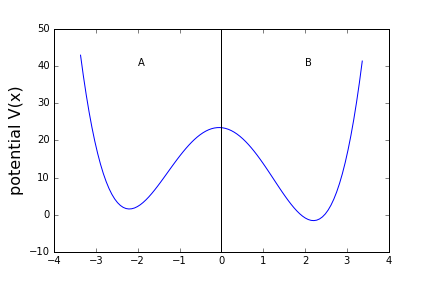
\includegraphics[width=0.6\textwidth]{Python/doublewell.png} %70% der Textbreite
	\caption{Full-partition of a double-well potential}
	\label{fig:doublewell}
\end{figure}
We are interested if the induced process $\xtilde_k$ inherits the Markovianity of $X_t$ or if it contains any memory effects.
%contains/includes

For a small lag-time $\tau = 0.1$ we compute the probability of $\xtilde_k$ to make a transition from $B$ to $A$ in one time-step. We compare it to the probability of the same transition with the \textbf{additional} information of having been in $B$ one time-step before/earlier. If the process was Markovian, then this additional information about the past should make no difference and thus, both probabilities should be equal.
We compute them in terms of the original process $X_t$ by
\begin{equation*}
\Prob_\mu[X_{(k+1)\tau} \in A \mid X_{k\tau} \in B] \textrm{ and }
\Prob_\mu[X_{(k+1)\tau} \in A \mid X_{k\tau} \in B, X_{(k-1)\tau} \in A].
\end{equation*}
Using the density functions $v_B$ and $v_{BA}$, we get \marginpar{$v$ densities?}
\begin{equation}
\label{eq:recrossing1}
\Prob_\mu[X_{(k+1)\tau} \in A \mid X_{k\tau} \in B] = \int_A v_B^\tau(x) \diff x = ... ,
\end{equation}
\begin{equation}
\label{eq:recrossing2}
\Prob_\mu[X_{(k+1)\tau} \in A \mid X_{k\tau} \in B, X_{(k-1)\tau} \in A] = \int_A v_{BA}^\tau(x) \diff x = ... .
\end{equation}
So we see that for such a short lag-time $\tau$, the process $\xtilde_k$ is \textbf{not} independent of the past  and hence \textbf{not} a Markov process.
%the process $\xtilde_k$ is \textbf{not} memoryless
%That behaviour is intuitively clear.
Equation \eqref{eq:recrossing1} describes the probability to get from $B$ to $A$, where ``being in $B$'' could mean everything from ``close to the transition region'' to ``far away from the transition region''. So this probability is averaged over \textbf{all} possible starting points in $B$. \marginpar{?}
We compare it to \eqref{eq:recrossing2}, where being in $A$ shortly before
%immediately one time-step; moving to B
being in $B$ increases the probability to return/recross to $A$ again.
This behaviour can be interpreted such that for a short time after a \textbf{transition}, the process is likely to be still inside ot the \textbf{transition region}.
In our example, the transition region is the area/region close to the maximum of potential energy. Thus, there is still an increased probability to return to the previous state.
%not only for this example true

%transition between states = crossing the ``barrier'' between the states..

%the probability that the process is still in the transition region. And to get to $A$ from the transition region in $B$ is just more likely than from any other region inside $B$.
%favorable spatial situation?

This issue is called the \textit{recrossing effect}, since additional memory \marginpar{recross the barrier?}
%as in \eqref{eq:recrossing2}
leads to an increased probability to ``recross'' shortly after a transition.
%when still being inside a transition region.
On the other hand, if we choose a large lag-time $\tau = 100$, then the past transition from $A$ to $B$ in \eqref{eq:recrossing2} took place a long time ago. So we cannot certainly know if the process is still in the critical transition region; during that long lag-time it could also have been gone anywhere else.
%That means that we could describe the memory effect of $\xtilde$ as a \textit{short-time memory}.
That means that the memory effect included in $\xtilde_k$ becomes smaller for larger lag-times and thus can be considered as a \textit{short-time memory}.

\subsubsection*{Comparison to Markov State Model}

After having observed the \textit{recrossing effect} as a memory effect when projecting the time-series(?) of a given continuous process onto a finite subspace, we want to compare that result to the corresponding \textit{Markov State Model}. \marginpar{def MSM}

So far, we considered the process $\xtilde_k$ belonging to the operator $G(\Pcal^k)$.
%Now, we want to consider the Markov State Model, i.e. the process $\xhat_k$ which is described by the operator $(G(\Pcal))^k$. The corresponding matrix representation is given by $P_c$ (see theorem \ref{thm:galerkin}).
Now, let $(\widehat{X}_k)_{k\in\mathbb{N}}$ be the Markov chain that is described by the transition matrix $P_c$, i.e. the matrix representation of the discretized transfer operator $G(\Pcal) := G\Pcal G$.
\\

A desirable behaviour of this model would be that $\widehat{X}_k$ and $\widetilde{X}_k$ have the same trajectory when started on the same initial distributions $\widehat{X}_0$ and $\widetilde{X}_0$. It will turn out that this is normally not the case.
%Another desirable property would be Markovianity of both models, since this is the case for the original process $X_t$. But we have alredy seen in theorem \ref{thm:galerkin} that the matrix representation $P_c$ of $G\Pcal G$ is in general not a transition matrix, i.e. $\widehat{X}_k$ is not Markovian
%shown/visualized
This question is visualized in diagram \ref{fig:diagram_transfer}.
Does it make a difference if we first project the process and then propagate it and vice versa?

\begin{figure}[!ht]
	\centering
	\begin{tikzcd}
	&  \Pcal(\tau) \arrow{d}{proj.} \arrow{r}{\tau \rightarrow \tau k}    & (\Pcal(\tau))^k \arrow{d}{proj.} 			\\
	G(\Pcal(\tau)) \widehat{=} &  P_c (\tau)   \arrow{r}{\tau \rightarrow \tau k}            &  (P_c(\tau))^k \\
\end{tikzcd}
\caption{Projecting/propagating a transfer operator (non-commutative)}
\label{fig:diagram_transfer}
\end{figure}
%\ref{fig:diagram_transfer}
%Weber shows in habilitation that under a certain Galerkin Projection using membership functions (not    %set-based family) leads to a commuting diagram of projection and propagation. \marginpar{non-reversible?}
%+ Markov Property is preserved? \marginpar{due to proj. or trans.op.?}
In general, this diagram is \textbf{not} commuting and hence, in general we have
\begin{equation*}
(P_c)^k \neq (P^k)_c.
\end{equation*}

For the example of a full-partition discretization, we know from section \ref{sec:galerkin} that the resulting Markov State Model is a Markov chain. Thus, we have a Markov chain $\xhat_k$ as a model for the non-Markovian process $\xtilde_k$, so it is clear that there is a discretization/iteration error.
%Thus, with this choice of membership functions, an accurate description of the real process is not possible
%maybe we should look our for better membership functions, s.t. P_c describes the evolution of the process

That is also where the term \textit{Markov State Model} comes from. We are describing the non-Markovian process $\widetilde{X}_k$ by a Markov chain $\widehat{X}_k$.
Originally, processes have been clustered \textit{set-based}, i.e. based on a full partition and thus always resulting in a Markov chain. In chapter \ref{chap:meta}, we will see that the \textit{function-based} approach yields better results and hence is the current state of the art. Then, the Markov State Model is not necessarily Markovian, as we already know from $P_c = TS^{-1}$ in theorem \ref{thm:galerkin}.

%corresponding to the projected process is not a a transition matrix. So in the normal case, neither of  %prop-proj and proj-prop. are Markovian! But can still differ! Which we are going to examine at the end of this %section.

%\subsubsection*{Example: Double Well Potential}

%Comparing that to $\xhat$. $\xhat$ is a Markov chain on the two possible states (=partition sets). Its transition matrix consists of the transition probabilities between these two sets within time $\tau$.
%But as these probabilities are built from an originally continuous state space, they are just averaged over the whole space. That means, the probability to get from $A$ to $B$ under $\xhat$ is always the same which is not an appropriate description of the original process. In fact/for instance, being in the transition region (i.e. close to $x=0$) inside of $A$ yields a much higher probability to get into $B$ in comparison to start inside of the energy minimum of $A$. But these differences are not included in our Markov State Model.


\subsubsection*{Discretization Error (Density Propagating Error/Iteration Error)}
\marginpar{what about eigenv. err.?}
%However
We will describe here shortly how the discretization error can be estimated. For our purposes that will not play an important role, since later we will be able to perform a projection (with convenient membership functions) s.t. this error vanishes. \marginpar{membership fct = part. of unity for clustering}
%we can zurückgreifen on a transfer operator by Weber\cite{weber2011subspace} which allows a projection without(?) error.

%discretization/ projection/ propagating error
The maximal possible error between the distributions of $\widetilde{X}_k$ and $\widehat{X}_k$ after $k$ time-steps is (independently of initial distribution) given by \marginpar{which norm?}
\begin{equation*}
E(k) = \Vert G(\Pcal^k) - (G (\Pcal))^k\Vert.
\end{equation*}

\begin{thm}
Assume the discrete/dominant spectrum of a transfer operator $\Pcal$ is given/denoted/ordered by $1=\lambda_0 > \lambda_1 \geq \dots \geq \lambda_n$. Then the projection error can be bounded from above in terms of the second-largest eigenvalue by
\begin{equation*}
\Vert (G (\Pcal))^k - \Pi_0\Vert \leq \lambda_1^k,
\end{equation*}
where $\Pi_0$ is the orthogonal projection of ... .
\end{thm}

For a proof, see Sch\"utte and Sarich\cite[p.72]{schutte2013metastability}.
%illuminating
In the following chapter we will see further/deeper relations between the spectrum of the transfer operator and ... properties.
%Furthermore, there is a relation between smallness of the  projection error and the metastability of a %subdivision of the state space.
%Schuette, Huisinga. Or Sarich p.58
\marginpar{def MSM, $P_c$}
We will see how to choose partition for a MSM s.t. the approximation error becomes small/vanishes. \marginpar{?}

\subsubsection*{Conclusion}

%What is the recrossing effect??? That the process loses its Markovianity?
%Iteration Error = that there is a deviation %between project/propagate and propagate/project?

We have to distinguish between two kind of ``errors'' that can occur:
\begin{itemize}
\item Rebinding Events: Projection can include some kind of memory effect
\item Iteration Error: Deviation of $G(\Pcal^k)$ and $(G(\Pcal))^k$
\end{itemize}

%\chapter{Metastability and Dominant Structures}
%\chapter{Dominant Structures in Markov Processes}
\chapter{Dominant Structures}\label{chap:meta}
% in Markov Processes
  %method/technique
With the Galerkin discretization, we introduced a method to reduce the dimension of a Markov process by projecting it onto a smaller state space.
However we don't know yet how to choose a partition of unity such that this projection yields a reasonable Markov State Model, in the sense that important properties of the original process are maintained.
%inherited,maintained
%by metastability, by a metastable behaviour, metastable sets
Usually, the long-time behaviour of a process is of particular interest. It is often determined by a so called metastable behaviour.
%It describes the typical behaviour of rare transitions between specific subsets, called \textit{metastable} or \textit{dominant subsets}, after a long duration of stay inside.
We will see why it makes sense to project a process onto its metastable sets and, in order to detect them, analyze their relation to the dominant spectrum of the transfer operator.
We will also see that the optimal metastable decomposition is not sharp/crisp but soft/fuzzy.
%in terms of membership functions

%introduce/present. decompose the state space/cluster a process/create a MSM
Additionally, with the aid of the Schur decomposition we introduce a rather new approach to create a Markov State Model. In contrast to the spectral approach, it includes nonreversible processes and is even able to identify further structures.
%cluster a broader class of processes.


\section{Metastability}
\label{sec:metastability}

There exist several definitions of metastability. %different definitions
%Shortly said, metastability is the property of a process that its state space consists of subsets/regions such that transitions between these subsets are rare events while the duration of stay inside of each of them is rather long.
Shortly said, metastability is the property of a process to act on particular regions such that transitions between these regions are rare events while the durations of stay inside of each of them is rather long.
%these subsets is rather long.
Some possible characterizations of that behaviour are based on large hitting times or small exit rates, see Sch\"utte and Sarich\cite[chapter 3]{schutte2013metastability},
where a good overview of the most common definitions can be found.
%which gives a good overview of the most common definitions.

\subsubsection*{Mathematical concept of metastability}

%define, introduce. $A \in \Sigma$?
In order to describe the concept of metastability, it is a good way to start with so called \textit{stable} or \textit{invariant subsets}. A measurable subset $A \subset E$ of the state space of a Markov process $X_t$ is called stable or invariant if it cannot be left, i.e. if $\Prob(X_t \in A \mid X_0 \in A) = 1$ for all $t$.
%Similarly
Analoguously, we can define a \textit{metastable} or \textit{almost invariant subset} as a subset in which the process will stay for a very long time before exiting it into any other subset, that is $\Prob(X_{t_f} \in A \mid X_0 \in A) \approx 1$ for a convenient timescale $t_f$.
%Metastability: A subset is not invariant but almost invariant
%Consequentially
Thus, a full partition $A_1,\dots,A_n$ of the state space $E$ is called \textit{metastable} if
\begin{equation}
\label{eq:metastability}
\sum_{k=1}^n \Prob_\mu(X_{t_f} \in A_k \mid X_0 \in A_k) \approx n.
\end{equation}
%mu??
Then each of the sets $A_k$ is almost invariant with respect to timescale $t_f$;
the probability to stay in one of the partition sets being started there is almost $1$, while the probability to change between any two different partition sets is almost $0$.
Such a partition is also called a \textit{metastable decomposition}.
%of the state space?

Obviously, being ``close to 1'' or ``close to $n$'' are rather vague statements.
However, that lack of concreteness will be eliminated later, since we will only be interested in the ``best'' metastable decomposition.
%That means that we want to obtain a decomposition where the sum \eqref{eq:metastability} is as close as possible to $m$, or equivalently the probability to stay inside of a metastable set is as close as possible to $1$.
%High holding probability?
That means that we want to obtain a decomposition where the probability to stay inside of each metastable set is as close as possible to $1$, resulting in the sum \eqref{eq:metastability} being as close as possible to $n$.
Likewise, the choice of the timescale $t_f$ is not specified in general and will depend on the particular system in consideration.
%has to be specified for each model individually. system/question in consideration/investigation/case
Hence, the only parameter in \eqref{eq:metastability} that has to be determined is the number $n$ of subsets we are looking for.
%\marginpar{joint metastability?}

\subsubsection*{Metastability in molecular systems}

Metastability is a very important concept for stochastic processes corresponding to molecular systems. Such processes describe the movement of atoms or molecules in space and
have the characteristic behaviour to oscillate or fluctuate around equilibrium positions on the smallest time scales (about one femtosecond). \marginpar{BM?}
In contrast to these fast oscillations, the process often stays inside of a certain region, called \textit{conformation}, for a long time before switching to another region (nano- or millisecond time scale).
%%switching/changing/exiting. region/subset. comparatively/relatively
Since transitions between conformations are relatively rare events, they can be identified as metastable sets if we choose a convenient timescale.
Such a behaviour is depicted in figure \ref{fig:conformations} on the example of the dihedral angle of a molecule, taken from Weber\cite{weber2011subspace}.

%\marginpar{conformation = spatial arrangement? special case of metastability?}
% long duration of stay + small transition rates/probabilities/ rare transitions between these subsets

\begin{figure}[!htb]
	\label{fig:conformations}
	\centering
	\includegraphics[width=0.7\textwidth]{conformations.jpg} %70% der Textbreite
	\caption{Example of a molecule with two (metastable) conformations. The dihedral angle of the molecule can take values between $+45^\circ$ and $-45^\circ$. There are two regions, highlighted red and blue, where the process stays for a rather long time and oscillates \textbf{inside}. Transition between these regions don't occur often. Thus, these two conformations can be identified as metastable sets.}
\end{figure}


%This dihedral angle can take values between $+45^\circ$ and $-45^\circ$.
%Thus, the process acts on a continuous state space and has infinitely many states.
%There are two regions, highlighted red and blue, where the process stays for a rather long time and oscillates \textbf{inside}.
%Transition between these regions don't occur often.
%and that transitions between these regions are rare.
%Thus, these two conformations can be identified as metastable sets.
%(metastable) conformations.

%useful
As transitions between metastable sets are rare events, long-time simulations of a process are required in order to get informations about conformational changes.
%%Thus, conformational changes are rare events and will show up only in long term simulations of the dynamics (nano- or millisecond time scale).
%complex systems
However long-time simulations of such large systems are not feasible in reasonable time even with the best computers nowaday, see Anton\cite{shaw2009millisecond} or its successor Anton$2$\cite{shaw2014anton}.
%supercomputers, designed for the purpose of such molecular dynamic simulations. %Unfortunately..

%needed/required
Hence, in order to be able to compute some long-time simulations of a given molecular system, a reduction of complexity  is needed. This can be achieved by a clustering of the state space via a Galerkin projection as depicted in section \ref{sec:galerkin}. Different states will be clustered appropriately such that we get a process on a smaller state space.
%depicted, described
\\

This point of view also motivates the following terminology. A state in the original state space is called a \textit{micro state}, as it is a state considered on the microscopic or atomistic level. In order to get a smaller state space, micro states are grouped together and such a cluster is called a \textit{macro state}, since we are now considering the process on a macroscopic level (cannot distinguish between smaller states/atoms anymore).

For instance, the spatial coordinates of a single atom could be considered as a micro state, while the corresponding macro state is a cluster of several atoms. If we are working on this smaller state space, we cannot distinguish anymore between the single atoms of the cluster (forget information).

\subsubsection*{Clustering into metastable sets}

%(i.e. how to choose the partition of unity for Galerkin projection)
%represents the correct long-time behaviour of the original process
The question \textbf{how} to cluster a given process such that it maintains the long-time behaviour of the original process can be answered easily with the following intuitive approach: As the long-time behaviour of a process is described by the metastability of the system, we choose the metastable sets as clustering sets.
%described, determined, based
More clearly, we create a new process where each macro state corresponds to one of the metastable sets.
In order to represent the correct long-time behaviour of the original process, the transition probabilities of the clustered process/reduced model should correspond to the transition rates between the metastable sets.
\\

%clusters/macro states/membership fcts.
%projected model

%cluster/group together
%As we are mainly interested in the long-time behaviour of a given process, it seems reasonable to cluster states of a metastable set together and create a new process where each macro state corresponds to one of the metastable sets. The transition probabilities of the clustered process/reduced model should correspond to the transition rates of the original process between its metastable sets. \marginpar{micro/macro states}
%between the macro states
%In order to..
%maintains, inherits, keeps
%determined in terms of
As metastability is determined on
%As metastability describes a behaviour on
%reduced model/projected process/clustered process
long timescales, the projected process maintains the long-time behaviour of the original process, but forgets about short-time transitions, i.e. transitions inside of a conformation/metastable set.

Since there is not one unique metastable decomposition of the state space, we need to find a decomposition which is in some sense ``the best''; then we can use it to create a reduced model. In the next sections we will see how to find such a decomposition.
\\

%clustering not unique: different metastable decompositions
%For example: in which metastable set should we assign a
%transition region (e.g. a region which is close to several metastable sets). SOLVED BY MEMBERSHIP?

%Going from micro states to macro states.

%\subsubsection*{Advantages / Disadvantages}

%projected/clustered
%reduced dimension/complexity
Most importantly, the clustered process will have the desired property of a reduced complexity since the model acts on a smaller state space.
%while maintaining the crucial property of the original process (transitions between metastable sets = long-time behaviour).
Therefore, the computation effort for long-time simulations is definitely decreased.
Furthermore, we get a better overview of the system, since it is always easier to consider a process on a few states in comparison to a process on a very large or even continuous state space.
However, it has to be guaranteed that the clustered process represents the \textbf{correct} long-time behaviour of the process. How this can be ensured will be explained in section \ref{sec:fuzzy}.
\clearpage
  \section{Spectral Approach}
\label{sec:spectral}

%connected,related
%In this section we show that the spectrum of the transfer operator is highly connected to the metastability of the corresponding Markov process.
In this section, we demonstrate the strong relation of the metastability of a Markov process to the spectrum of the associated transfer operator. %associated/corresponding
%spectrum of the transfer operator to the metastability of the corresponding Markov process.
More precisely, the existence of metastable sets implies the existence of dominant eigenvalues of the transfer operator and vice versa.
The idea to detect metastable sets via dominant eigenvalues has been first proposed by Dellnitz and Junge\cite{dellnitz1999approximation} and transferred to molecular dynamics by Sch\"utte et al\cite{schutte1998conformational,schutte1999direct}.

\subsubsection*{Existence of dominant eigenvalues}

%The \textit{multiplicity} of an eigenvalue $\lambda$ is defined as the dimension of the generalized %eigenspace. Eigenvalues of multiplicity $1$ are called  \textit{simple}.

%Let us, lag-time t
We consider the transfer operator $\Pcal := \Pcal(\tau)$ of a Markov process for some fixed lag-time $\tau$ in the Hilbert space $L^2(\mu)$. \marginpar{ $L^2$, $L^1$?}
%$L^1$ Huisinga diss; why $L^2$, $L^1$ enough?
%For further informations, see Kato\cite{kato1995}.
We are interested in \textit{dominant eigenvalues} of $\Pcal$, that is large eigenvalues which are close to 1 and separated from the rest of the spectrum.
The \textit{discrete spectrum} $\sigma_{\mathrm{discr}}(\Pcal)$ is the set consisting of all eigenvalues $\lambda \in \sigma(\Pcal)$ that are isolated and of finite multiplicity.
%contains all
The \textit{essential spectral radius} $r_{\mathrm{ess}}(\Pcal)$ is defined as
\begin{equation*}
r_{\mathrm{ess}}(\Pcal) = \inf \{ r \geq 0 \mid \lambda \in \sigma(\Pcal) \textrm{ with } |\lambda| > r \textrm{ implies } \lambda \in \sigma_{\mathrm{discr}}(\Pcal) \}.
\end{equation*}
%essential/continuous. under consideration
The existence of dominant eigenvalues requires that the continuous part of the spectrum is bounded away from the dominant elements of the discrete spectrum.
To ensure that the process we are considering actually possesses metastable sets, we need to pose some conditions on the spectrum of the transfer operator:
\begin{description}
    \item[C1] The essential spectral radius of $\Pcal$ is less than one, i.e. $r_{\mathrm{ess}} < 1$.
    \item[C2] The eigenvalue $\lambda=1$ of $\Pcal$ is simple and dominant, i.e.
    %i.e. $\eta \in \sigma(\Pcal)$ with $|\eta| = 1$ implies $\eta = 1$.
    \begin{equation*}
    \eta \in \sigma(\Pcal) \textrm{ with } |\eta| = 1 \textrm{ implies } \eta = 1.
    \end{equation*}
\end{description}
%criteria for it
We will not go into further details for which processes the two above conditions are fulfilled; some criteria can be found in Huisinga\cite[chapter $4$]{huisinga2001metastability}.
Since we are interested in a metastable behaviour, we assume that the processes under investigation satisfy these conditions.
%Since these conditions are required for the later investigations, we will just assume that they are true.
We need condition {\textbf{\textsf{C1}} to ensure that the continuous part of the spectrum is bounded away from the discrete eigenvalues. Otherwise they would not be dominant anymore and the process would be rather rapidly mixing than having any metastable sets.
%metastable sets/dominant structures
Condition {\textbf{\textsf{C2}} however is important because the state space of a transfer operator with more than one eigenvalue of absolute value $1$ can be decomposed into invariant sets, that is subsets which cannot be left. \marginpar{absolute?}
%\marginpar{C2 = ergodic?}
%\marginpar{has periodic structures?}
%stable/invariant
However, such a case is not interesting for us.
%\marginpar{excludes modeling and interpretation problems}
Instead, we want to know more about \textbf{almost} invariant sets and their critical transition regions. 
%We will consider only ergodic process which means theat the eigenvalue $1$ is unique.
\\


%transfer operator for a process unique?
The transfer operator $\Pcal: L^2(\mu) \rightarrow L^2(\mu)$ of a reversible process satisfying the properties \textrm{\textbf{\textsf{C1}}} and \textrm{\textbf{\textsf{C2}}} is self-adjoint by theorem \ref{thm:selfadjoint_reversible} and has a spectrum of the form
%has a spectrum of the form/the following spectrum
%\marginpar{why discr. rechts?}
\begin{equation*}
\sigma(\Pcal) \subset [a,b] \cup \{\lambda_n\} \cup \dots \cup \{\lambda_2 \} \cup \{1\}
\end{equation*}
with $-1 < a \leq b < \lambda_n \leq \dots < \lambda_1 = 1$ and isolated, not necessarily simple eigenvalues of finite multiplicity that are counted according to multiplicity.


\subsubsection*{Relation of dominant spectrum to metastability}

%state,determine
In order to find out about the quality of an arbitrary decomposition, we present upper and lower bounds for the metastability of the decomposition in terms of dominant eigenvalues and eigenvectors of the transfer operator.
We will denote by \textit{metastability of a decomposition $\Dcal$} the sum of the metastability of its subsets.

%Sch\"utte\cite[theorem 4.16]{schutte2013metastability}
\begin{thm}[{Huisinga and Schmidt\cite[Theorem 2.4]{huisinga2006metastability}}]
\label{thm:metastability_bounds_1}
Let $\Pcal$ be the transfer operator of a reversible process satisfying \textrm{\textbf{\textsf{C1}}} and \textrm{\textbf{\textsf{C2}}}.
Let $\lambda_1,\dots,\lambda_n$ denote its isolated eigenvalues and $v_1,\dots,v_n$ the corresponding eigenfunctions, normalized to $\Vert v_i \Vert_2 = 1$.
Let $Q$ be the orthogonal projection of $L^2(\mu)$ onto $\mathrm{span}\{\eins_{A_1},\dots, \eins_{A_n}\}$.
The metastability of an arbitrary decomposition $\Dcal = \{A_1,\dots, A_n\}$ of the state space $E$ can be bounded from above by
\begin{equation*}
p(A_1,A_1) + \dots + p(A_n, A_n) \leq 1+ \lambda_2 + \dots + \lambda_n,
\end{equation*}
while it is bounded from below by
\begin{equation*}
1+ \rho_2 \lambda_2 + \dots + \rho_n \lambda_n + c \leq p(A_1,A_1) + \dots + p(A_n, A_n),
\end{equation*}
where $\rho_j = \Vert Q v_j \Vert_{L^2(\mu)}^2 = \langle Qv_j, Qv_j \rangle \in [0,1]$ and $c = a(1-\rho_1) \cdots (1 - \rho_n)$.
\end{thm}

%shows,reveals. relation/connection. eigenfunctions and eigenvalues
Theorem \ref{thm:metastability_bounds_1} reveals the strong relation between metastable sets and the dominant eigenvalues of the transfer operator.
%enables,allows,provides us an insight into. evaluate,judge,rate
It allows us to evaluate the quality of a decomposition by comparing the lower and the upper bound of metastability.
The upper bound shows that eigenvalues far away from $1$ worsen the metastability of a decomposition.
The lower bound is close to the upper bound if the dominant eigenfunctions $v_2,\dots,v_n$ are almost constant on the metastable subsets $A_1,\dots,A_n$, implying $\rho_j \approx 1$ and $c \approx 0$.
Moreover, Huisinga and Schmidt\cite{huisinga2006metastability} show that the lower and upper bounds from theorem \ref{thm:metastability_bounds_1} are sharp and asymptotically exact.

That provokes the question if there exists an \textbf{optimal} decomposition with the highest possible metastability. \marginpar{maybe ill-conditioned}
%In fact, this problem might unfortunately be ill-conditioned.
By all means, this theorem indicates that the number of metastable sets should be determined by the number of dominant eigenvalues.
\\

Deuflhard et al\cite{deuflhard2000identification} proposed an algorithm to identify the metastable sets of a Markov chain by exploiting the sign structure of the dominant eigenvectors of the transition matrix.
\\

In figure \ref{fig:spectrum}, we get a good overview of the relation between the eigenfunctions of the transfer operator and the metastable sets of the corresponding process. We have a potential/energy landscape with 4 energy minima, that is 4 regions where the process could be \textit{trapped} such that it is hard to get outside again. The transition matrix  shows this metastable behaviour since we can see 4 regions which large probabilities to stay inside and very small probabilities to go to a different region.
Furthermore we see that the process has 4 dominant eigenvalues. Three of them have a change of sign, inducing a metastable decomposition.
\newpage


\begin{figure}[!ht]
	\label{fig:spectrum}
	\centering
	\subfigure[Transition matrix $P$ on $100$ states with $4$ visible metastable sets]{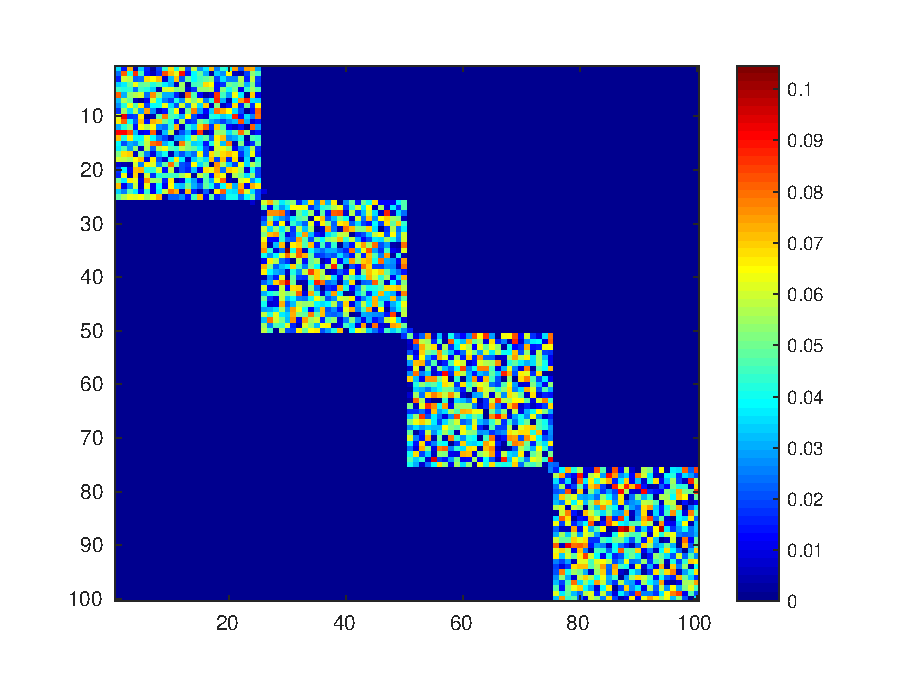
\includegraphics[width=0.49\textwidth]{figures/spectral/transition.eps}}
	\subfigure[Spectrum of $P$ with $4$ dominant eigenvalues]{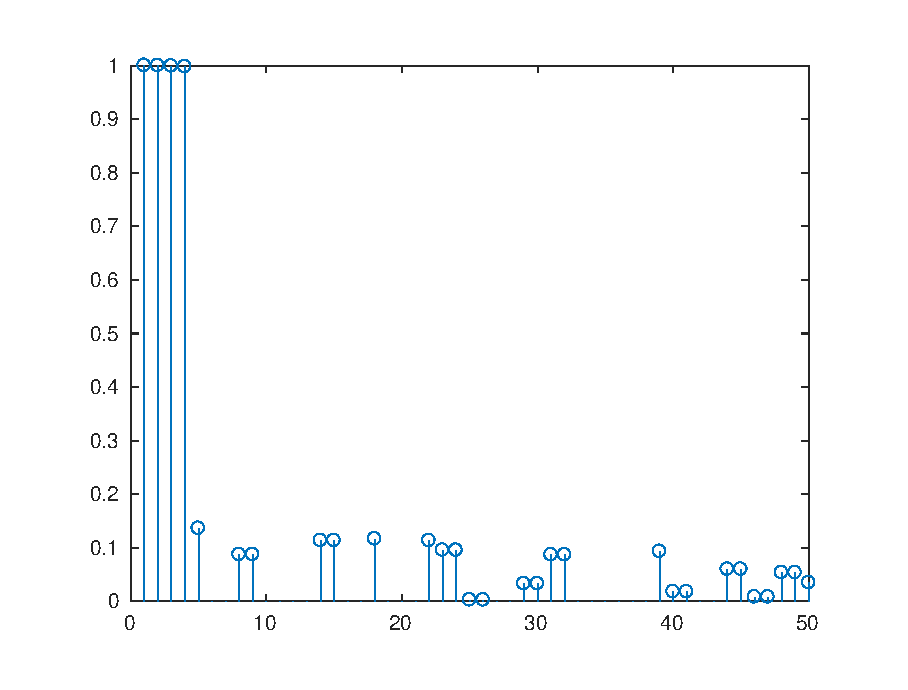
\includegraphics[width=0.49\textwidth]{figures/spectral/eigenvalues.eps}}
	\subfigure[Dominant eigenvectors of $P$ with change of signs corresponding to the transition regions]{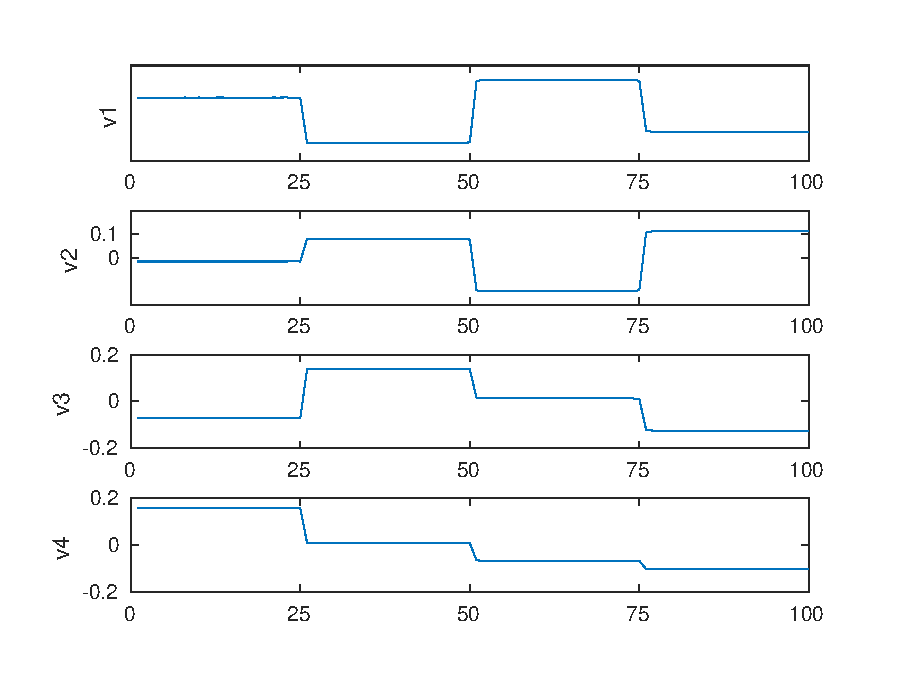
\includegraphics[width=0.49\textwidth]{figures/spectral/eigenvectors.eps}}
	\caption{Relation of the transition matrix to its spectrum with regard to metastability}
\end{figure}

%anschaulich
%This theorem gives us a first demonstrative relation of the metastability of a process to its eigenvectors. This %result is not yet optimal/very good. In the next sections, we will see that linear combinations of eigenvectors %result in much better metastability.


This relation can be explained as follows.
A process consisting of $n$ invariant sets $\{A_1,\dots,A_n\}$ has the $n$-fold eigenvalue $1$ and the corresponding eigenvectors $\eins_{A_i}$ are constant on the invariant sets.
A metastable process consists of almost invariant sets and thus, can be interpreted as the perturbation of a process with invariant sets, by introducing small transitions between the invariant sets. Accordingly, the eigenvalues and eigenvectors are perturbed. This results in one eigenvalue $1$ and $n-1$ eigenvalues close to $1$, having eigenvectors that are almost constant on the almost invariant sets.
A detailed perturbation analysis can be found in Deuflhard et al\cite{deuflhard2000identification}.

\subsubsection*{Disadvantages}
%Conclusion
%Advantages, Alternatives

%suitable,convenient
%to characterize metastability of Markov processes, respectively. wrt its metastable sets
%convenient,suitable,possible,feasible
The spectral approach is an appropriate method to cluster a process with respect to metastability, though it bears some disadvantages.
%1:
The result is only appliable on reversible processes, because real eigenvalues are only guaranteed if the transfer operator is self-adjoint. \marginpar{see}
%2:
%Moreover, the eigenvector problem of the transfer operator has only global solutions. \marginpar{global = good?}
%Most of all,
Particularly, the previous procedure to compute a metastable decomposition does not take into consideration the existence of transition regions.
This can lead to an iteration error, i.e. the clustered process does not represent the correct long-time behaviour.
%needs refinement/improvement
\\

%clarify/point out/emphasize/highlight
This section has been presented mainly with the aim to emphasize the strong relation of the spectrum of the transfer operator to the metastability of the system. %mainly/merely/solely/only
%results in a full partition decomposition and
However, this approach does \textbf{not} represent the state of the art.
%This relation can be seen best for a full partition decomposition/clustering.
%enhanced/improved. related, but improved,
In the next section, we deduce an enhanced method, resulting in a \textbf{soft} clustering instead of a full partition decomposition.
%, which likewise takes advantage of this strong relation between spectrum and metastability.
%It also includes the eigenvalues and eigenfunctions of the transfer operator, but will be soft instead of crisp.
%comprises/includes the eigenvalues and eigenfunctions of the transfer operator, but it will be fuzzy.

  \section{Fuzzy Clustering}
\label{sec:fuzzy}

%(metastable decomposition induced by zeros of eigenfunctions)?
The above considerations result in a metastable full decomposition of the state space, assigning each state to \textbf{exactly} one of the partition sets.
%taking into consideration
%Now we show that
In fact, there exist better solutions, considering the fact that states in transition regions are adjacent to several conformations and therefore cannot be uniquely assigned to one of them.
%can belong to several metastable conformations.
We introduce a more general method, allowing some ``overlap'' of the conformations.
%metastable sets/conformations
%in the assignment of states to conformations.
%wer hat diese Methode introduced?? see...
%there may be some overlap in the assignment of states to metastable sets.

% a transition region can be %assigned to several macro states with different weight/degree/probability

\subsubsection*{Set-based vs. Function-based Approach}
The intuitive approach to decompose the state space of a process is to determine a certain number of metastable sets which form a full partition, such that each state belongs to exactly one of the metastable sets.
%is assigned, belongs
%each partition corresponds to one conformation/ metastable set.
The problem with that approach is that likewise each state in a transition region has to be assigned to one of these partition sets. Though why would you assign a state in a transition region to one particular adjacent metastable set and not to another one? Such a strict assignment is obviously not an accurate description of the actual behaviour of the process.
%rigorous,precise,accurate

Therefore this \textit{set-based} clustering method has been replaced by a \textit{function-based} method.
That means that the states of the process are assigned with certain ``degrees'' to the conformations.
This approach is justified by the existence of transition regions.
A state inside of a transition region (around local energy maximum) can enter into different adjacent conformations with similar probabilities.
Therefore, instead of assigning it to a single conformation, we define that it should belong to each of these adjacent conformations with a certain degree.
% and thus, can be interpreted to belong to these conformations with a certain degree.
%maybe it cannot be uniquely assigned to a single conformation.
In that sense, the conformations may be ``overlapping''.


\subsubsection*{Membership Functions}

%reversible
Assume we are given a transfer operator having $n$ dominant eigenvalues. Hence, we want to create a Markov State Model on $n$ states, corresponding to the metastable sets of the process.
We follow the approach of Weber\cite{weber2006meshless} to define macro states as \textit{overlapping partial densities}.
%Each macro state is identified by a membership function $\chi_j$ that assigns to each micro state a degree of membership to belong to this conformation.
They can be identified by membership functions that assign degrees of membership to the micro states.
%signifying

%Each state of the original state space shall be assigned to the different macro states with a certain \textit{degree of membership}.

%So far, we were speaking about partition of unity, but with the fuzzy terminology in mind it makes sense to call them membership functions; as they determine the portion of membership to each conformation
\begin{defi}[Membership Function]
% (see \ref{sec:galerkin})
The functions $\cfam : E \rightarrow [0,1]$ are called \textit{membership functions} if they fulfill
\begin{itemize}
\item $\chi_j(x) \geq 0$ $\forall i \in E$ and $\forall j \in \{1,\dots,n\}$ (positivity),
\item $\sum_{j = 1}^n \chi_j(x) = 1$ $\forall x \in E$ (partition of unity).
\end{itemize}
The value $\chi_j(x)$ is the \textit{degree of membership} of state $x$ to macro state $\chi_j$.
%\marginpar{conf. $j$ or $\chi_j$?}
\end{defi}
%membership fct. = part. of unity? Here: yes. Röblitz: required that each function takes value 1

The example of a full-partition discretization corresponds to the choice of characteristic functions $\{ \eins_{A_1},\dots, \eins_{A_n} \}$ as membership functions. Each micro state is uniquely assigned to one of the partition sets, without any overlap.
Therefore such a clustering is called \textit{crisp} or \textit{hard}, whereas the general, possibly overlapping, membership functions result in a \textit{fuzzy} or \textit{soft} clustering.
As there are many possible membership functions, we need to find a choice that yields a reasonable metastable decomposition.
%Usually they look like that

%It turns out that a good choice are membership functions that are
Usually they are chosen to be \textbf{close} to a characteristic function, also called \textit{almost characteristic function}, as depicted in \ref{fig:fuzzy}.
%region,conformation. reasonable/makes sense
%This choice makes sense,
This is a reasonable choice, since it puts the emphasis of a conformation on a certain region by assigning a high degree of membership,
%and maybe some adjacent parts (low degree of membership), but also takes into consideration the critical behaviour of transition regions.
though likewise includes the adjacent transition regions by a low degree of membership.
Thus, they fulfill the following two desired conditions:
\begin{itemize}
\item There should be a \textbf{soft} assignment inside of a transition region, in order to respect the ambiguous membership of transition states.
%Transition regions should be handled carefully, i.e. there should be a \textbf{soft} assignment,
\item The clustering should be \textbf{crisp} enough to distinguish the conformations.
%Different conformations should be clearly visible, so the clustering should be \textbf{crisp} enough to distinguish the conformations.
\end{itemize}

\begin{figure}[!ht]
	\centering
	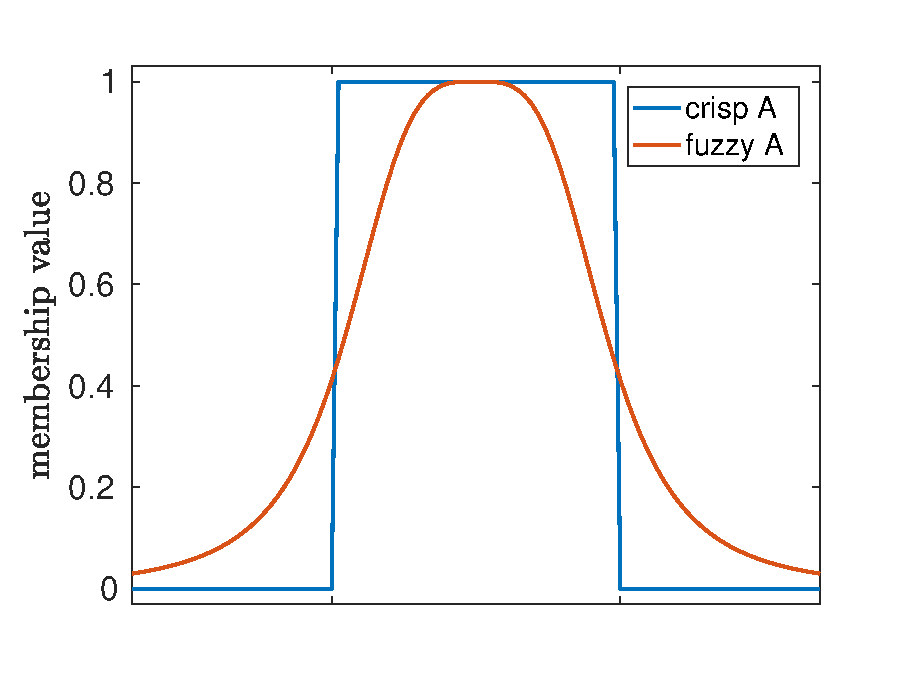
\includegraphics[width=0.4\textwidth]{figures/fuzzy/fuzzy3.eps}
 	\caption{The crisp set $A$ represented by a characteristic function is approximated by a fuzzy set represented by an ``almost characteristic function''.}
        \label{fig:fuzzy}
\end{figure}

These requirements are clarified in figure \ref{fig:membership} at the recurring example of a double-well potential, i.e. a system consisting of two conformations with one transition region between them. A crisp clustering does not consider the transition region, while a ``very fuzzy'' choice of membership functions does not represent the conformations.

\begin{figure}
	\centering
	\subfigure[Characteristic functions resulting in a hard clustering.] {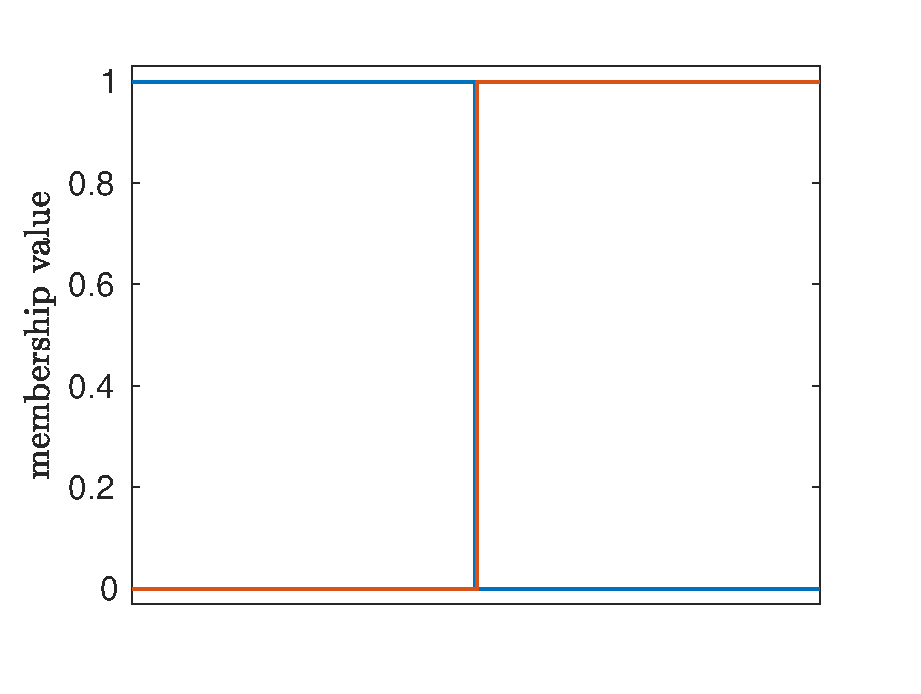
\includegraphics[width=0.4\textwidth]{figures/fuzzy/indicator2.eps}}
	\subfigure[Almost characteristic functions resulting in a soft clustering.]{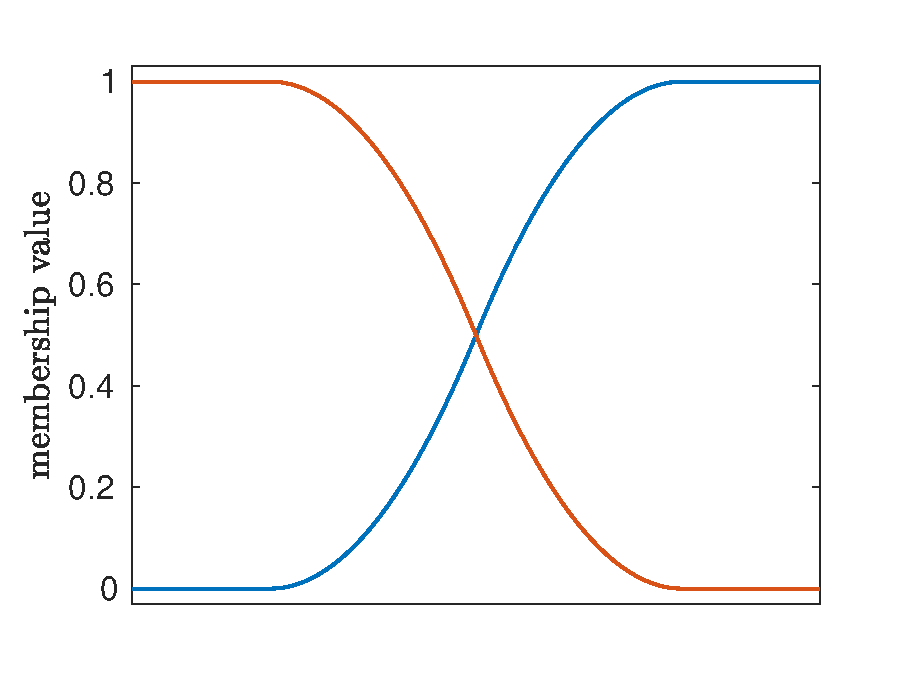
\includegraphics[width=0.4\textwidth]{figures/fuzzy/almost2.eps}}
%	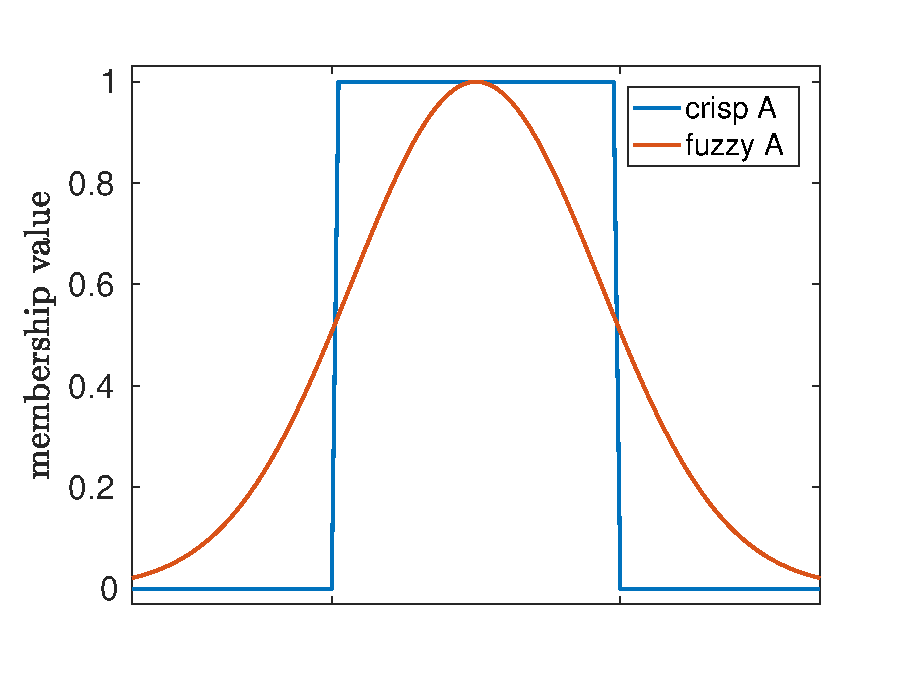
\includegraphics[width=0.3\textwidth]{figures/fuzzy}
	\caption{Possible membership functions: From hard to fuzzy clustering.}
	\label{fig:membership}
\end{figure}

%Conceptually, they are no probabilities
The degrees of membership are no actual probabilities, yet they can be interpreted as such.
%In the case of a full-partition discretization, the probability of a micro state to belong to a certain conformation is $1$, while the probability to be in any other conformation is $0$, which is obvious by the unique assignment of micro states to the conformations.
Consider for instance the energy maximum of a symmetric double well potential. This transition state tends with the same probability to the left and to the right well. Therefore it seems plausible to assign it with the same degree of membership to both conformations.
On the other hand, a state in the middle of a well cannot immediately jump into the other well, therefore this transition probability is $0$ and the state can be assigned with degree of membership $1$ to the conformation corresponding to its well.
\\

%improvement/enhancement. fuzzyness/overlap
%In figure \ref{fig:membership}, we can clearly see the advantage of using almost characteristic functions as membership functions. Since they allow a soft assignment of the transition region, they are an improvement in comparison to characteristic functions.
%Nevertheless, the functions should not be ``too fuzzy'', since otherwise the disctinction between the conformations can be blurred. Thus some overlap is good, but we also need a certain crispness, in order to identify different conformations.
%identify,distinguish

%another way to explain the meaning of membership functions; interpretation as partial densities
For each conformation $j \in \{ 1 , \dots, n \}$, there is a membership function $\chi_j$ which determines the portion of the partial density with respect to the total density function. \marginpar{?}
They form a partition of unity, in order to sum up to the total density.
%Sometimes the $\chi_j$ will also be called conformation.
In the following, the $\chi_j$ will also be denoted as the conformation $j$ they represent.
%some density function given? t.ex. Boltzmann distribution
%Weber Diss 10
\\

In order to represent the conformations as almost invariant sets, almost characteristic functions should be almost eigenfunctions of the transfer operator:
%having invariant sets
%As characteristic functions are right eigenvectors of a uncoupled(!) transition matrix, the following should be true for almost characteristic functions, thus for membership functions: \marginpar{??}
%perturbation analysis
\begin{equation*}
\Pcal \chi_j \approx \chi_j \ \forall j=1,\dots,n.
\end{equation*}
%\begin{equation*}
%\Qcal \chi_j \approx 0 \ \forall j=1,\dots,n.
%\end{equation*}
%\begin{equation*}
%P_c \chi_j \approx \chi_j \ \forall j=1,\dots,n.
%\end{equation*}
%\begin{equation*}
%T\chi_j \approx S\chi_j \ \forall j=1,\dots,n.
%\end{equation*}
%\pagebreak

%Meaning of the Matrix Representation of the Galerkin Projection
%\subsubsection*{Galerkin Projection} %(Matrix Representation)
\subsubsection*{Matrix Representation of Projection} %(Matrix Representation)

Having determined the shape of the membership functions, we can apply the Galerkin projection as defined in section \ref{sec:galerkin}.
If we choose almost characteristic functions representing the (fuzzy) conformations, then the resulting Markov State Model consists of the metastable sets of the original process.
%represents the metastable sets of the original process
%More precisely, each membership function is an almost characteristic function representing a fuzzy conformation. \marginpar{?}
We remember the matrix representation $P_c = S\inv T$ of a clustered process.
The trace of the coupling matrix $T$ is referred to as \textit{metastability} of the conformations $\{\cfam\}$.
%why that makes sense? high diagonal elements -> high eigenvalues -> high metastability
%Weber meshless p.26

We recall that a full-partition decomposition yields a matrix $S$ being equal to the identity matrix, justified by the orthogonality of the characteristic functions. With the motivation to choose almost characteristic functions as membership functions, the $\chi_i$ are still close to being orthogonal and therefore, $S$ should still be close to the identity matrix, at least diagonal dominant. \marginpar{..}

Thus, we have the coupling matrix $T$, representing the dynamical behaviour of the process.
%Since it should consist of the metastable sets, it should also be a diagonally dominant matrix.
%Now, what is the actual meaning of $S$? Does it ``disturb'' the stochastic matrix $T$ in some sense?
If $S$ is close to the identity matrix, then the dynamics of the projected process is completely determined by $T$. In contrast, if $S$ deviates from identity, then it rather influences the dynamics.

What is the meaning of $S$? The entries are defined by the scalar products of the membership functions.
Thus, the \textit{crispness} of a clustering can be measured by the matrix $S$.
% nonoverlapping = char. fcts.
Nonoverlapping membership functions yield an overlap matrix $S$ equal to the unit matrix.
Overlapping membership functions result in a matrix with non-zero outer diagonal elements.
The higher the outer diagonal elements, the higher the overlap.
Therefore the diagonal of $S$ can be seen as a ``measure of crispness'' of the $\chi_1,\dots,\chi_n$. % conformations/membership functions
%Individual eigenfunctions $\Xcal$ do not overlap since they are orthogonal. But the membership functions %$\chi_j$ as linear combinations of the dominant eigenfunctions might have an overlap.
\\

%\subsubsection*{Statistical Weights} %\marginpar{what for?}

%For each macro state we can assign a statistical weight
Each macro state yields a statistical weight
\begin{equation*}
w_j = \langle \chi_j, \eins \rangle_\mu = \int_E \chi_j(x) \mu(\diff x),
\end{equation*}
describing the ``portion'' of a membership function to the total density function. \marginpar{?}
We remark that the statistical weight vector $w = (w_1, \dots, w_n)$ coincides with the left eigenvector of the matrix representation $P_c$ of the clustered process, see theorem \ref{thm:lefteigenvector}.
%stationary vector/left eigenvector of the clustered process
The diagonal matrix $D = \mathrm{diag}(w_1,\dots,w_n)$ consists of the statistical weights of the membership functions. Then $S = D\inv \langle \chi, \chi \rangle_\mu$ and $T=D\inv \langle \chi, \Pcal \chi \rangle_\mu$, compare theorem \ref{thm:galerkin}. %\marginpar{$TS\inv$ vs $S\inv T$}


\subsubsection*{Perron Cluster Analysis} %\marginpar{finite/cont. vec./fct.}

The term \textit{Perron Cluster Analysis} denotes the objective of clustering a Markov process into metastable sets using the \textit{Perron eigenvalues} respective \textit{Perron eigenfunctions}, being eigenvalues close to $1$ and the corresponding eigenfunctions. %means/denotes
Perron Cluster Analysis respectively its algorithmic implementation PCCA (``Perron Cluster Cluster Analysis'') has been developed by Deuflhard et al\cite{deuflhard2000identification}, employing the sign structure of the dominant eigenvalues of the transition matrix. %\marginpar{set-based approach?}
%as what?
%That approach
This has been improved by Deuflhard and Weber\cite{deuflhard2005robust}
%\marginpar{oder Weber und Galliat?}
%soft/fuzzy
who transformed the system of eigenvectors into a system of membership functions resulting in a fuzzy clustering of the state space of the original process; their algorithm is called PCCA+
(``Robust Perron Cluster Analysis'').
%adapted
Originally, PCCA+ was formulated only for discrete Markov chains, but Weber\cite{weber2011subspace} extended it even on continuous processes.
%we present here the more general case for cont. processes with a given transfer operator
\\

%Let $\Xcal$ be the eigenvector matrix, \marginpar{eigenfct.?} i.e. the $i$-th column of $\Xcal$ is an %eigenvector corresponding to the eigenvalue $\lambda_i$. \marginpar{only dom. spec.}

Let $\Pcal := \Pcal(\tau)$ on $L^2(\mu)$ be the transfer operator describing a \textbf{reversible} process, that is $\Pcal$ is $\mu$-self-adjoint, see theorem \ref{thm:selfadjoint_reversible}.
We consider the set of dominant eigenvalues $\{\lfam\}$ with the corresponding set of eigenfunctions $\Xcal = \{\xfam\}$.
They fulfill the eigenvalue problem $\Pcal \Xcal = \Xcal \Lambda$ of the transfer operator $\Pcal$, where $\Lambda = \mathrm{diag}(\lfam)$.
The set of membership functions $\chi= \{\cfam \}$ can be built as a linear combination $\Xcal \Acal$ of the dominant eigenfunctions, that is
\begin{equation}
\label{eq:pcca}
\chi_j(x) = \sum_{i=1}^n \Acal_{ij} \Xcal_i(x), \ j=1,\dots,n.
\end{equation}
%properties/constraints
Here,  $\Acal = \{\Acal_{ij}\}_{i,j=1,\dots,n} \in \R^{n\times n}$ is a real matrix which has to be chosen in such a way that the resulting membership functions $\chi$ fulfill the positivity and partition of unity constraints.
%Noe Lecture 4 (MSM 2015) 
As there are infinitely many such transformations $\Acal$ of the eigenfunctions, we have to determine one that satisfies some optimality condition.
%resulting in a soft membership matrix,
%Consequently,
The algorithm PCCA+ computes the transformation matrix $\Acal$ as the solution of a \textbf{convex} maximization problem, see Weber\cite{weber2006meshless}. %\marginpar{optimal metastability?}
%yields
%In order to fulfill the partition of unity property of each $\chi_i$, the matrix $A$ has to be chosen s.t. $\chi$ %is row-stochastic.
With the resulting membership functions, the Galerkin projection is %computed/given by %(see chapter 1)
\begin{equation}
\label{eq:galerkin2}
	P_c(\tau)  = G(\Pcal(\tau)) = (\langle \chi, \chi \rangle_\mu)\inv (\langle \chi, \Pcal(\tau) \chi \rangle_\mu).
\end{equation}

%\marginpar{only conv. lin.comb.}
Weber\cite{weber2011subspace} shows that for any linear combination of the eigenfunctions $\chi = \Xcal \Acal$, the discretization error of the Galerkin projection vanishes. Hence diagram \ref{fig:diagram_transfer} commutes, implying that propagating and projecting of a transfer operator are commutative actions. In particular, such membership functions preserve the Markov property.
%In particular, such a choice of membership functions preserves the Markov property.
%Markovianity
\begin{thm}[Weber {\cite[Theorem 2]{weber2011subspace}}]
	\label{thm:iteration_error}
	Let $\Pcal := \Pcal(\tau)$ be a $\mu$-self-adjoint transfer operator with a set $\Xcal = \{ \Xcal_1,\dots, \Xcal_n\}$ of normalized eigenfunctions s.t. $\Pcal \Xcal = \Xcal \Lambda$, where $\Lambda = \mathrm{diag}(\lambda_1,\dots,\lambda_n)$ is the eigenvalue matrix.
	Let $\chi = \Xcal A$ be a set of functions that is a linear combination of the eigenfunctions $\Xcal$ with a regular $n \times n$-transformation matrix $A$ as defined in \eqref{eq:pcca}.
	Then the iteration error for the Galerkin discretization $P_c = G(\Pcal)$ vanishes. %in \eqref{eq:galerkin2}
\end{thm}
\begin{proof}
	%weber p.32
	%We compute the Galerkin projection on the transfer operator $\Pcal$:
	The Galerkin projection of the transfer operator $\Pcal$ is computed by
	\begin{align*}
	G(\Pcal) \; & \stackrel{\mathclap{\eqref{eq:galerkin2}}}{=}  \;
	(\langle \chi, \chi \rangle_\mu)\inv (\langle \chi, \Pcal \chi \rangle_\mu) \\
	& \stackrel{\mathclap{\eqref{eq:pcca}}}{=} \;
	( A^T \langle \Xcal, \Xcal \rangle_\mu A)\inv ( A^T \langle \Xcal, \Pcal \Xcal \rangle_\mu A) \\
	& = \; ( A^T \langle \Xcal, \Xcal \rangle_\mu A)\inv ( A^T \langle \Xcal, \Xcal \rangle_\mu \Lambda A) \\
	& = \; ( A^T A)\inv ( A^T \Lambda A) \\
	& = \; A\inv \Lambda A.
	\end{align*}
	In particular, after $k$ time-steps we get
	\begin{equation*}
		(G(\Pcal))^k = (A\inv \Lambda A)^k = A\inv \Lambda^k A = G(\Pcal^k).
	\end{equation*}
	%Besides
	%\marginpar{semigroup prop.?}
	The last two lines are obtained by inserting the eigenvalue problem $\Pcal \Xcal =\Xcal \Lambda$ and employing the $\mu$-orthogonality of the eigenfunctions, by theorem \ref{thm:spectrum_operator}, and therefore $ \langle \Xcal, \Xcal \rangle_\mu = \Ical$, being the identity operator. \marginpar{orthogonal by symmetrization trick?}
	%The proof is based on the assumption that the Perron eigenfunctions of $\Pcal$ are orthogonal.
\end{proof}

In this proof, it is essential that the process is reversible. If the process is non-reversible, then the transfer operator is not self-adjoint and possibly possesses complex eigenvalues, leading to complex-valued eigenfunctions, which can not be transformed into meaningful membership functions. %spanning invariant subspace of P
%then the orthogonality of the dominant eigenfunctions is not given anymore. \marginpar{not real}
Thus, in order to tackle non-reversible processes as well, an enhanced method is presented in section \ref{sec:nonreversible}.
%it is necessary to introduce a different concept (section \ref{sec:nonreversible}).
\\

%Nielsen p.37!!!!!

%since computation of eigenfunctions is not easy
Even though the algorithm of PCCA+ is valid for continuous processes defined by a transfer operator $\Pcal$, for real applications a discretization of $\Pcal$ to a matrix $P$ is necessary:
\begin{equation*}
	\Pcal \rightarrow P \rightarrow P_c.
\end{equation*}
% of the state space $E$
One approach for that are direct sampling methods, counting transitions between subsets. However, since long-time simulations are required in order to obtain valuable informations about transition between metastable sets, they are not the best choice. Another option are adaptive sampling methods, for instance Voronoi tesselation, see Weber\cite{weber2011subspace}. \marginpar{?}
Having a discrete matrix $P$, it is easy to compute the eigenvalues and eigenvectors in order to apply PCCA+ to get a clustered matrix $P_c$.
In this thesis, we circumvent this first discretization step, by directly examining finite matrices $P$. %are not confrontated

%If we project a finite process, then the above formulation yields a \textit{membership vector matrix} $\chi$, which is the result of a linear combination of the \textit{eigenvector matrix}.
%\newpage

\subsubsection*{Objective Function: Crispness of Membership Functions}
%Weber Diss 58

%Moreover, 
The matrices $S$ and $T$ from the matrix representation $P_c$ can be expressed as
\begin{equation}
\label{eq:projection_presentation2}
\begin{aligned}
T & = D^{-1} \langle \chi, \Pcal \chi \rangle_\mu = D^{-1}A^T \Lambda A \ \ \textrm{ and } \\
S & = D^{-1} \langle \chi, \chi \rangle_\mu = D^{-1} A^T A.
\end{aligned}
\end{equation}

Different objective functions are possible, some are proposed in Weber\cite[Chapter 3.4]{weber2006meshless}.
Originally, one objective was to maximize metastability by maximizing $\mathrm{trace}(T)$.
In the context of stochastic matrices, a high trace of corresponds to a high determinant, since $\trace(T)$ is bounded by above from $n$ and $\det(T)$ by $1$.
This upper bound is achieved only for the case of the identity matrix, thus for a ``strong diagonal''.
Trying to increase the trace to being close to $n$ is the same as increasing the determinant to being close to $1$.
Since the trace is not multiplicative, we resort to the determinant to calculate the following relation:
\begin{align*}
\det(T) & = \det(S) \det(A\inv \Lambda A)  \\
		  & = \det(S) \det(\Lambda)			 \\
          & = \det(S) \Pi_{i=1}^n \lambda_i.
\end{align*}
In order to obtain a high metastability of the system, both factors need to be high.
%In order to increase the metastability of a system, both factors need to be high.
%determinants need to be high.
The term $\det(\Lambda)$ is high if the dominant eigenvalues $\lambda_i$ are as close as possible to $1$, whereas $\det(S)$ is maximized if the linear combination $\chi = \Xcal \Acal$ is as \textbf{crisp} as possible.
That means that they are as orthogonal as possible, having only few overlap.
Since $S$ is a stochastic matrix as well, maximizing its determinant is equivalent to maximizing its trace.

%makes sense
Thus the choice of maximizing $\trace(S)$ as objective function for PCCA+ is plausible, since it provides a clustering with high metastability, while the metastable sets are well distinguishable because of the crispness.  This was proposed by R\"oblitz\cite{roblitz2009statistical}.
Moreover, $\trace$ is a \textbf{convex} function, which is a necessary criterion for the objective function of PCCA+:
\begin{equation}
\label{eq:crispness}
\max_{A \in \R^{n \times n}} \trace(S) \ \ \textrm{such that} \ \chi = XA \geq 0 \ \mathrm{and} \ \sum_j \chi_{ij} = 1. 
\end{equation}
%\\

%Different objective functions are possible. The intuitive optimization criterion would be to maximize the metastability of the membership vectors such that the resulting clustering is ``optimal'' with respect to metastability. However, a different optimization criterion is to make the membership vectors as ``crisp'' as possible by maximizing the trace of the matrix $S$.
%That means that they should be as orthogonal as possible. This was proposed by R\"oblitz\cite{roblitz2009statistical}.
%Thus the objective function used in PCCA+ is given by
%PCCA+ solves the constrained optimization problem

%The trace of $S$ is at most $n$. Optimizing $\mathrm{trace}(S)$ is equivalent to optimizing the \textit{crispness} of the conformations $\chi$ (Röblitz). -> high metastab.

%Better: linear combination of eigenfunctions (might have an overlap) (membership functions, PCCA+).

\subsubsection*{Example}
\clearpage
  \section{Dominant Cycles}
%(non reversible NESS process)
\label{sec:nonreversible}

When it comes to computing a metastable decomposition for a nonreversible process, we have to face the problem that the eigenvalues/eigenvectors might be complex valued and thus, PCCA+ is not applicable. \marginpar{of transf.op.?}
One possibility/alternative/way to circumvent this problem is to consider the real Schur decomposition of the matrix(?) instead of its spectral decomposition. Then, we can apply PCCA+ to the real Schur vectors of the matrix instead to its eigenvectors.
This approach is feasible/possible, since the real Schur vectors span the same subspace as the corresponding complex Schur vectors and those span the same subspace as the corresponding eigenvectors. \marginpar{see ...}

%In this section, we give an overview about a special case of nonreversible processes (NESS); nonreversible but having a steady state/stat. dist./stat. meas.

%In addition, additionally
Furthermore, a nonreversible process can contain other dominant structures than just \textit{metastable sets/conformations}. It can as well contain \textit{metastable cycles}, that is subsets with a cyclic behaviour and a high probability to stay inside of such a cycle for a long time.
%structures/subsets

%In general, there exist two possible ways to uniquely describe a Markov chain; via a transition matrix or via cycles.

\subsubsection*{NESS processes}

%We begin with introducing a certain class of processes that are nonreversible, but still have some nice properties.

\begin{defi}[NESS process]
A Markov process is called \textit{nonequilibrium steady state (NESS)} process if it is nonreversible, but still has a steady state, \marginpar{what is that?} given by an invariant measure $\mu$ w.r.t. which the process is ergodic.
\end{defi}

$p_\tau(A,B) = p(\tau,A,B) =  \Prob(X_\tau = B \mid X_0 = A)$

As a NESS process is nonreversible, there are regions where the detailed balance equation is not fulfilled, i.e. there is an effective probability flow $p(\tau, A, B) - p(\tau,B,A) \neq 0$ between some subsets $A,B \subset S$ of the state space.

\subsubsection*{Flow of a process}
\marginpar{why only finite?}

In the following we consider an irreducible and aperiodic (i.e. ergodic) Markov chain on the finite state space $S= \{1,\dots,n\}$ given by the transition matrix $P$. Since this Markov chain is irreducible and aperiodic, it possesses a unique invariant measure $\mu$ that is positive everywhere. \marginpar{see ..}
Then $\mu$ is the normalized eigenvector of $P$ for the unique eigenvalue $\lambda = 1$.

\begin{defi}[Flow Matrix]
The probability flow associated to a Markov process is given by the flow matrix
\begin{equation*}
F = DP,
\end{equation*}
where $P$ is the transition matrix of the process and $D$ the diagonal matrix $D_{ii} = \mu_i$ with the entries of the invariant measure $\mu$.
\end{defi}
So the (steady state) probability flow from state $i$ to $j$ is given by $F_{ij} = \mu_i P_{ij}$.
If the process is reversible, the flow matrix $F$ is symmetric due to the detailed balance equation. For a NESS process, $F$ is not symmetric since there are states $i,j \in S$ with $F_{ij} \neq F_{ji}$.

\subsubsection*{Cycle Decomposition}

This flow must be decomposable into elementary cycles. \marginpar{why?}

\begin{defi}[Cycle of a process]
A $k$-cycle $\gamma$ on $S$ is an ordered sequence (up to cyclic permutations) of $k$ connected states $\gamma = (i_1,\dots,i_k)$ with length $|\gamma| = k$, i.e. the probability to get to the next state is always positive: $\Prob_{i_j, i_{j+1}} > 0$ and $\Prob_{i_k,i_1} > 0$.
\marginpar{1-step prob.?}
Cycles without repetition/self-intersections are called simple cycles. The set of all simple cycles is denoted by $\Ccal$.
\end{defi}

We want to make a cycle decomposition of the flow $F$, see Kalpazidou\cite{kalpazidou2007}.

\begin{defi}[Cycle/flow Decomposition]
A collection $\Ccal_+ \subset \Ccal$ of cycles $\gamma$ with real positive weights $w(\gamma)$ is a flow decomposition if for every edge $(i,j) \in S^2$ we have
\begin{equation*}
F_{ij} = \sum_{\gamma \supset (i,j)} w(\gamma),
\end{equation*}
where $(i,j) \subset \gamma$ if the edge $(i,j)$ is in $\gamma$.
\end{defi}

In order to make sense in a probabilistic context, we define the weight $w$ of a cycle $\gamma$ in the following way. Given a (realization of?) Markov chain $(X_t)_{t \in \T}$, we count the number of times $N_T^\gamma$ the process passes through a cycle $\gamma$ up to time $T$.
%w will be the mean/average number of the appearances of c along almost all the sample paths

\begin{defi}[Weight of a Cycle]
\begin{equation*}
w(\gamma) = \lim_{T \rightarrow \infty} \frac{N_T^\gamma}{T}.
\end{equation*}
\end{defi}
Since we are considering/assuming an ergodic process, this limit exists a.s. \marginpar{jian qian}


\subsubsection*{Dominant cycles/sets}
%[djur] chap 5
%same as PCCA+ but for nonreversible processes, so with Schur vectors instead of eigenvectors

We will see that dominant cycles have similar properties as dominant sets for reversible processes, i.e. large eigenvalues with $|\lambda| \approx 1$. But now the eigenvalues are lying in the complex plane and might be non-real (pairs of complex eigenv.).

%What is a metastable cycle?
\begin{defi}[Dominant Cycle]
= metastable cycle?
\end{defi}

So a cycle is dominant if there is a high probability inside the Markov chain to follow this cycle.

%What is the dominant structure of a nonreversible process? ibland cycle, ibland set?
%What is egentligen the problem with nonreversible processes? non-real eigenvalues

Dominant structures will be defined utilizing the dominant Schur vectors
of the transition matrix instead of its eigenvectors.
A membership matrix can be defined as a linear combination of these leading Schur vectors (spectral clustering with PCCA+).

%\subsubsection*{Spectrum of a NESS process}

\subsubsection*{Schur Decomposition}

We have the same situation/aim as in the previous sections: we have a Markov process on a large state space $S$ and we want to decompose it into a smaller state space consisting of clusters that belong to dominant structures of the process.

%Schur Decomposition = Matrix Decomposition

\begin{defi}[Schur Decomposition]
Let $P \in \mathbb{R}^{n \times n}$ be a transition matrix. Then it can be written as
\begin{equation*}
P = XRX^{-1},
\end{equation*}
where $X$ is a unitary matrix and $U$ is an upper triangular matrix, which is called a \textit{Schur form/matrix/decomposition} of $P$.
\end{defi}

Since $R$ is similar to $P$, both matrices have the same spectrum. Since $R$ is triangular, their eigenvalues are the diagonal entries of $R$.

A Schur Decomposition is not unique. \marginpar{...}
As $P$ is a real matrix, its non-real eigenvalues come in complex conjugate pairs. This fact can be used to build a \textit{real Schur form}, where $X$ and $R$ are both real matrices. But then $R$ is no longer triagonal, but only \textit{quasi-triangular}, allowing $2 \times 2$-blocks on its diagonal. \marginpar{picture}
The eigenvalues of the $2\times 2$-blocks are exactly the complex conjugate eigenpairs of $P$. \marginpar{see ..}

\begin{thm}[Real Schur Decomposition {\cite[Exc. I.3.24]{stewart1990matrix}}]
%Röblitz p. 22
If $A \in \R^{N \times N}$, then there exists an orthogonal matrix $U \in \R^{N \times N}$ such that
\begin{equation*}
U^TAU = T,
\end{equation*}
where $T$ is block-triangular with $1 \times 1$ and $2 \times 2$-blocks on its diagonal. The $1 \times 1$-blocks contain the real eigenvalues of $A$ and the eigenvalues of the $2 \times 2$-blocks are the complex eigenvalues of $A$.
\end{thm}

\begin{defi}[Schur Vector]
Let $\widetilde{R} \in \mathbb{R}^{m \times m}$ be a submatrix of $R$ (top left part of $R$). Then
\begin{equation*}
P = \xtilde \widetilde{R} \xtilde^{-1},
\end{equation*}
where $\xtilde \in \R^{n \times m}$ consists of the first $m$ columns of $X$. These vectors will be denoted as the dominant Schur Vectors of $P$. \marginpar{why?} Schur Values?
\end{defi}

\subsubsection*{Using PCCA+}
Djurdjevac Conrad et al\cite{djur2016} propose an algorithm in order to determine/get the desired membership vectors $\chi$.
\begin{enumerate}
\item Compute a real Schur decomposition $(\xtilde, R)$ of ...
\item Sort the Schur values and the $2 \times 2$-blocks such that they are in a descending order
%according to their maximal absolut values
\item Determine the submatrix $\xhat$ and solve PCCA+ equation (...) in order to get the membership functions $\chi$
\end{enumerate}

\subsubsection*{Computation of metastable cycles/sets}

%I. Beckenbach, L. Eifler, K. Fackeldey, A. Gleixner, A. Grever, M. Weber, J. Witzig: Mixed-Integer Programming for Cycle Detection in Non-reversible Markov Processes(2017)
Fackeldey and Weber\cite{fackeldey2017gen}
%GenPCCA+
%M. Weber and K. Fackeldey.   G-PCCA: Spectral clustering for non-
%reversible markov chains. ZIB-Report 15-35, Zuse Institute Berlin, 2015

\chapter{Rebinding Effect in a Given Kinetics}\label{chap:rebinding}
  %In this chapter, we examine a particular type of molecular systems, namely receptor-ligand systems, consisting of special molecules, so called receptors and ligands.
In this chapter, we examine receptor-ligand-systems, a special type of molecular systems, consisting of so called receptors and ligands. %special/particular
These molecules can interact in such a way that under certain conditions they can bind to each other and afterwards dissociate again.
Such a system is originally Markovian and can be described by a transfer operator.
However, by projecting this operator onto a finite-dimensional state space, the Markov property of the process may be spoiled.

%introduce, present, explain. quantity, occurence
We explain this memory effect, the so called rebinding effect, and examine its influence on the stability of a receptor-ligand-system. We show how this effect can be measured with tools known from chapter \ref{chap:markov}. %its influence on the quantity of binding events of a receptor-ligand-system
In particular, we present a lower bound for the rebinding effect included in a given system as the solution of an optimization problem.
%We are particularly interested in analyzing an optimization problem to find a lower bound for the rebinding effect included in a given kinetics.

%emphasis, focus, is mainly based on, mathematically based. basic/fundamental. knowledge,notations,defs
This chapter highly complies with Weber and Fackeldey\cite{weber2014}.
Additionally, we introduce some fundamental definitions and notations from biochemistry, which are necessary for the understanding of receptor-ligand-systems.
The importance of such systems is illustrated by an outlook of its application in drug design. %becomes clear
%The meaning/importance/relevance of such systems becomes clear by a description/outlook of its application/uses for drug design.
%and involves an approach for nonreversible processes.
%also\cite{weber2012}?

\section{Receptor-Ligand System}
\label{sec:rebinding}

We present a particular molecular system, the \textit{receptor-ligand-system}, and model it mathematically using a differential equation.
We discuss the so called rebinding effect and set in in relation to the recrossing effect known from section \ref{sec:recrossing}.
%a memory effect occuring in this model,
%outlook for later/further investigations
As a motivation, we explain its relevance in the application of drug design.
%As an outlook/motivation.. important application of \textit{drug design} and how the rebinding effect can help to improve the effect/efficiency of drugs. \marginpar{?} NO? just reveals that in reality, we have higher binding affinity, than we thought?stillgood

\subsubsection*{Molecular Dynamics vs Molecular Kinetics}
%\marginpar{Weber p.10}
A molecular system consists of molecules, that are atoms which are connected by \textit{covalent bonds}.
%bla bla.
%The potential energy function, or \textit{energy landscape}, of a molecular system results in a dynamical behaviour on different timescales.
%The fastest timescales (vibrations of covalent bonds) are around $10^{-15}$ seconds. \marginpar{see ..}
%They can  range from 10^-15 seconds for the vibration of covalent bonds, to seconds or even longer (for instance protein folding, ligand binding))
%bla. up to nanoseconds or, for protein folding, up to microseconds or seconds or even longer..
%\\
The motion inside of such a system can be characterized in different ways.
%Such a system can be characterized in different ways. %described/analyzed/characterized
The term \textit{molecular dynamics} denotes the analysis of a \textbf{single} trajectory and is mainly employed in the context of simulations. \marginpar{?}
It means that one initial configuration of the system is fixed and its evolution in time is observed. One example is depicted in figure \ref{fig:conformations}.
It represents \textbf{one} trajectory of a stochastic system. This can give an insight about the structure of the system, like identifying possible metastabilities. However, it is not representative in the sense that a second simulation could yield a completely different trajectory.
In contrast to that, in \textit{molecular kinetics}, an \textbf{ensemble} of trajectories is considered.
Accordingly, it is formulated in terms of densities, concentrations or transition rates.
%These terms cannot be mixed with the trajectory-based approach. Sentences like "trajectory behaves according to transition rate" makes no sense
However, these quantities are related to the molecular dynamics approach as they represent an average of many single realizations of a process.
%These observables/quantities can be understood/interpreted as averages/result of many/infinitely many single rajectories.


\subsubsection*{Receptors and Ligands} \marginpar{references}

In biochemistry, a \textit{receptor} is a molecule, often a protein, that is usually located on the surface of a cell and can receive signals from outside the cell.
A molecule that has the ability to \textit{bind} or \textit{associate} to a receptor is called a \textit{ligand}.
Each receptor will only bind with ligands of a particular structure, which is often referred to as the ``key-lock principle''.
%lock-key
Both receptor and ligand need to have specific complementary geometric shapes that fit exactly into one another, as exemplarily depicted in figure \ref{fig:Protein_ligand_binding}.
%correct size, shape, and charge composition in order to bind and interact with the receptor.

%both of them have specific shape which has to fit to each other
\begin{figure}[!ht]
	\centering
	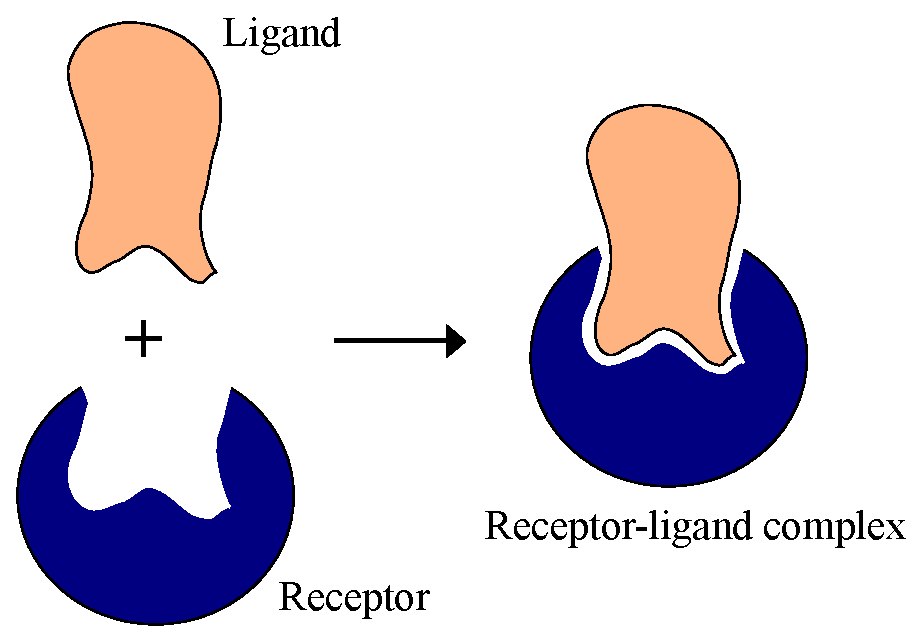
\includegraphics[width=0.5\textwidth]{figures/receptor_ligand.eps}
	\caption{Ligand (``key'') binds to a receptor (``lock''). Their shapes fit together.}
	\label{fig:Protein_ligand_binding}
\end{figure}

%produce,cause,lead to,provoke,trigger
Such a binding between a receptor and a ligand can \textit{activate} (``unlock'') the receptor by producing some kind of a chemical signal and thereby provoke a physiological response.
For instance, that could be a conformational change in a protein, caused by a hormone binding to it.
%binding energy can lead to conformational change in the receptor, %https://en.wikipedia.org/wiki/Ligand_(biochemistry)
%actual,possible consequences
However, instead of engaging in the actual physiological consequences of a binding, we focus on the \textbf{act} of binding events.
%Thus, we consider a \textbf{ligand binding process}.

%random movements of particles. Brownian motion?
%assume: well-stirred/mixed -> equilibrium. what if starting in non-equilibrium?
%in general, typically
The action of binding is typically reversible\footnote{We remark that in this context, \textit{reversible} means that a ligand can bind and unbind to a receptor, i.e. the reaction can run forward and backward.
%that is bound in a complex has the ability to dissociate from the complex and become unbound again.
In contrary to the mathematical reversible, which means that a process behaves \textbf{equally} when running backwards in time.} through \textit{dissociation} of the involved receptor and ligand.
Ligand binding is a \textit{chemical equilibrium} process, which means that the reaction rates of the binding and dissociating events are equal, once this equilibrium is reached.
From then on, the concentrations of the reactants (ligands) and the products (complexes) are constant.
It is a \textit{dynamic equilibrium}, since reactions take place, even though no net change in the concentrations can be observed.

The binding behaviour of a simple receptor-ligand system is formalized as follows. %\marginpar{kinetics}
A ligand (L) can bind to a receptor (R) and form a receptor-ligand complex (LR) which can dissociate again into its original components. This process can be represented by a reaction equation
%in the following form
\begin{equation}
\label{eq:reaction}
\mathrm{L} + \mathrm{R} \rightleftharpoons \mathrm{LR}.
\end{equation}
%implies,states
Being a process in chemical equilibrium, the law of mass action states that the ratio between the concentration of reactants and products is constant.
The corresponding \textit{dissociation constant} $k_d$ is given by
\begin{equation*}
k_d = \frac{\mathrm{[L]} \cdot \mathrm{[R]}}{\mathrm{[LR]}},
\end{equation*}
%free/unbound
where [L] is the concentration of unbound ligands, [R] is the concentration of unoccupied receptors and [LR]  is the concentration of receptor-ligand complexes.
%where [L], [R] and [LR] represent the concentrations of (L),(R) and (LR), respectively.
%relatively/proportionally
This constant is used to describe the \textit{binding affinity} between a ligand and a receptor, that is how strongly/tightly the ligand can bind to his particular receptor. If the dissociation constant is small, then there are relatively many complexes in comparison to unbound molecules, and for this reason, the binding affinity between the ligand and the receptor is high.
%Affinity is a measure of the tendency of a ligand to bind to its receptor.
The \textit{association constant} $k_a$ is just the inverse of the dissociation constant
\begin{equation*}
k_a = \frac{\mathrm{[LR]}}{\mathrm{[L]} \cdot \mathrm{[R]}}.
\end{equation*}
There are different factors which can influence the binding affinity of a process.
%Firstly, the attraction between receptor and ligand needs to be high. Furthermore, the binding strength needs to be high, that is dissociations should not happen often. ???
%\marginpar{affinity = anziehung + staying in bond + strong rebinding?} NO! only anziehung?
% reasons/values
%The dissociation constant for a particular ligand-protein interaction
It depends on the nature of the constituent molecules, like their shape, size and possible charge.
The binding affinity of a particular ligand-protein interaction can also change significantly with solution conditions (e.g., temperature, pH and salt concentration).
%thus, take a drug at a certain temperature
%These factors can depend on different parameters of the system, like temperature or PH value; but also on the nature of the constituent molecules, like their shape, size and possible charge.
%The rate of binding is called affinity, and this measurement typifies a tendency or strength of the effect.
%https://en.wikipedia.org/wiki/Ligand_(biochemistry)
%For example, a higher temperature leads to a faster movement of the molecules and therefore increases the probability of binding events. \marginpar{but also dissociates faster?}

In general, high-affinity binding results in a higher degree of occupancy for the ligand at its receptor binding site than is the case for low-affinity binding; the residence time (lifetime of the receptor-ligand complex) does not correlate. \marginpar{?}
%https://en.wikipedia.org/wiki/Ligand_(biochemistry)

\subsubsection*{Mathematical Model of Receptor-Ligand-System}

Starting from the reaction equation \eqref{eq:reaction}, we can deduce that the ligand can be found in two different macro states: ``unbound'' (L) or ``bound'' (LR). Then the probabilities of the ligand to be in one of these states can be described by the probability vector $x^T = \frac{1}{s}((\mathrm{[L],[LR]}))$, where $s = \mathrm{[L]} + \mathrm{[LR]} = \textrm{const.}$ is the normalization constant.
This leads to an ordinary differential equation
\begin{equation*}
\dot{x}^T = x^T Q_c.
\end{equation*}
The matrix $Q_c$ consists of the rates of reaction,
\begin{equation*}
Q_c = 
\begin{pmatrix}
-k_a[R] & k_a[R]  \\
k_d      & -k_d
\end{pmatrix},
\end{equation*}
where $k_a$ and $k_d$ are the association and dissociation constants. It corresponds to the transition rate matrix of a Markov chain, that means it describes a \textbf{memoryless} process.
We will later see that this mathematical description of a receptor-ligand-system is not accurate, since in fact, such a process \textbf{will} have some kind of memory.
%does not describe the actual/real long-time behaviour of the system

\begin{figure}[!ht]
	\label{fig:two_states}
	\centering
	\subfigure[Unbound]{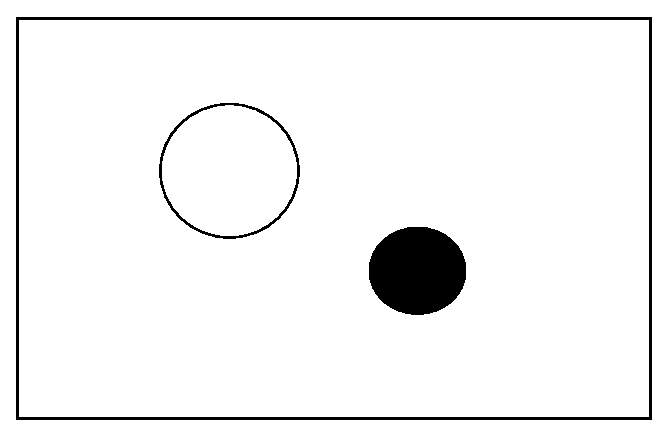
\includegraphics[width=0.25\textwidth]{figures/unbound.eps}}
	\hspace{20pt}
	\subfigure[Bound]{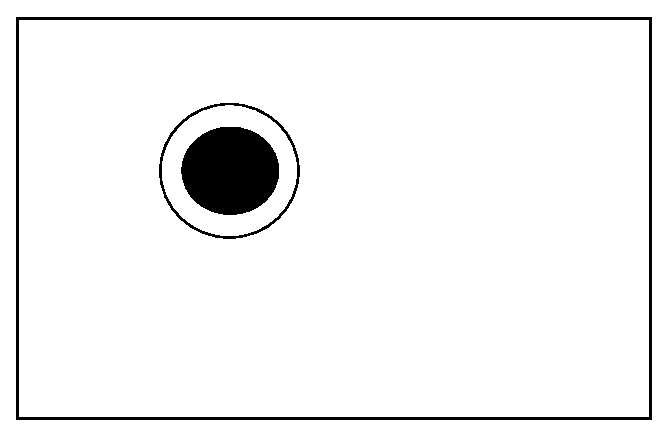
\includegraphics[width=0.25\textwidth]{figures/bound.eps}}
	\caption{Two possible macro states of a ligand-binding system}
	%(unbound, bound)
\end{figure}

The two possible macro states for the easiest case of a ligand-binding-system consisting of one receptor and one ligand are depicted in figure \ref{fig:two_states}. %We discover/detect/notice/remark
We notice that the spatial arrangement of the receptor and the ligand in the unbound case is \textbf{not} included in the above model.
%impact,consequences of that will be seen soon
Therefore, we cannot distinguish if, at a given time, the receptor and the ligand are close to each other or not.

\subsubsection*{Rebinding Effect}

%At the beginning/start, we assume that the molecules are rather good mixed and thus the probability for binding events is rather gleichverteilt.
%But after some time, bindings will occur. And that will lead to memory effects!

%The rebinding effect has been characterized as a \textbf{memory effect} which leads to an additional thermodynamic weight of the bound state.
%Weber quantifying rebinding effect
%occurs when projecting a MD process onto a finite subspace??

%assume: at the beginning well-stirred and thus abstände receptor-ligand gleichverteilt. drugs? :S
%tatsächlich,..
In fact, a stochastic process describing a receptor-ligand system is \textbf{not} necessarily Markovian.
That is due to the spatial arrangement of the system after the dissociating of a receptor-ligand-complex took place.
Shortly after such a dissociating, it is more likely that the corresponding receptor and ligand will bind again, since they are still close to each other.
Such a binding shortly after being dissociated is called a \textbf{rebinding}. The memory effect which thereby occurs is called \textbf{rebinding effect}.
%rebinding event. will vanish, diminish
On large timescales, this effect will vanish since the favorable spatial situation is not necessarily given anymore and the system will be rather mixed again.
%rebinding: rein mathematisch durch die Projektion entstanden?
%oder kann ein Prozess aus anderen Gründen mehr oder weniger Rebinding haben? multivalence
%can or IS spoiled? may be spoiled?
Thus, Markovianity can be spoiled by the rebinding effect.
It is depicted in figure \ref{fig:rebinding}.
\\


\begin{figure}[!ht]
	\label{fig:rebinding}
	\centering
	\subfigure[Spatial constellation shortly after dissociation. The ligand is still \textbf{close} to the receptor.]{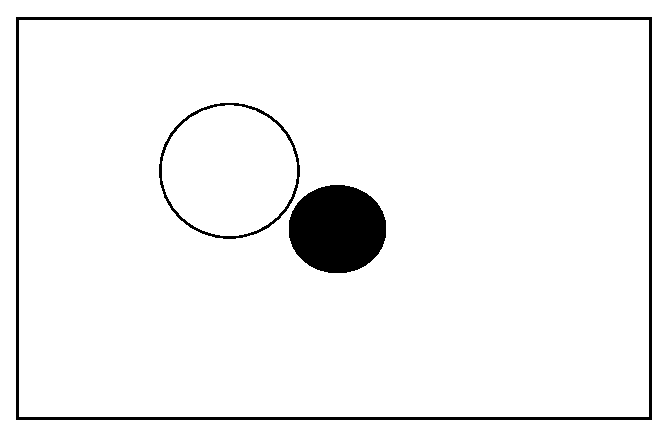
\includegraphics[width=0.25\textwidth]{figures/unbound2.eps}}
	%, increasing the probability of a fast \textbf{rebinding}.
	\hspace{20pt}
	\subfigure[Possible spatial arrangement long time after a dissociation.]{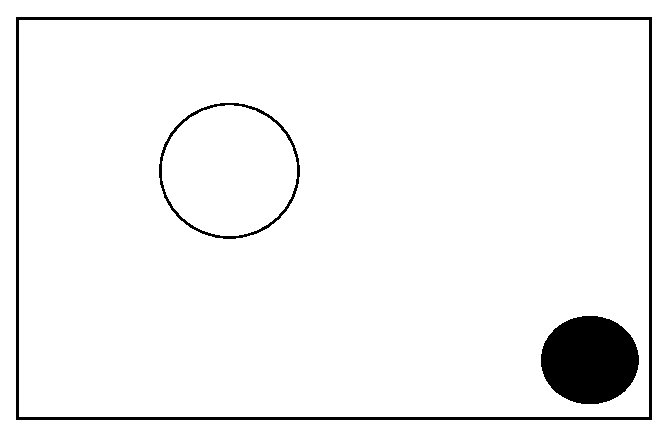
\includegraphics[width=0.25\textwidth]{figures/unbound1.eps}}
	\caption{Rebinding Effect. Two configurations of a system consisting of one receptor and one ligand, represented by the same macro state (``unbound'').}
	%receptor (white) and one ligand (black)
	%(unbound, bound)
\end{figure}

%in molecular systems
The rebinding effect and its occurence in natural science has been described and analyzed by several authors\cite{goldstein1995approximating, vauquelin2010}.
In chemistry, it has been discussed in the context of clustered receptors and clustered ligands\cite{care2011impact}. %\marginpar{multivalence}
%efforts,approaches. quantify the rebinding effect.  mathematical point of view
A mathematical description of the rebinding effect has been realized by Weber et al\cite{weber2012,weber2014}.
%as the rebinding effect occurs by the projection, i.e. by a mathematical concept
%embed it in mathematical context
% and a mathematical point of view.
%from a chemical and a mathematical point of view.

%In chemistry, there are several reasons/factors for the strength/quantity of the rebinding effect discussed (multivalency,..). \marginpar{only math; impact of multivalence}
%(Weber, Chem.)
%recently
The rebinding effect has been discussed to increase the binding affinity of a process.
\marginpar{?}


\subsubsection*{Rebinding Effect vs Recrossing Effect}
The characterization of the rebinding effect reminds us of  the recrossing effect, as described in section \ref{sec:recrossing}.
%We remember the description of the recrossing effect in section \ref{sec:recrossing}.
There, we considered the projection of a possibly continuous process onto a finite state space. This projected process (MSM) was described by a transition matrix, thus being a Markov chain, even though the process actually contained a (short-time) memory. \marginpar{it. error vs reb. eff.}
%There, we had a projected process on macro states described by a transition matrix and thus being a Markov chain. But in reality, the (clustered) process was not memoryless.
The same phenomena occurs with the rebinding effect.
We have a process which is \textbf{modelled} by a Markov chain, even though the process actually \textbf{has} a memory.
%We have a transition matrix, even though our process has a memory.
We can interpret the two states of the ligand-binding-system as macro states resulting from the projection of a process on a larger state space (for instance, including more informations about the spatial situation of the receptor and the ligand).
%(for instance, containing informations about the spatial coordinates of the (contributing) molecules).
In this case, the rebinding effect originates from the loss of information caused by the projection and therefore, qualitatively corresponds to the recrossing effect. %\marginpar{quant. same?}
\\

Thus, the rebinding effect coincides with the recrossing effect in the special context of a receptor-ligand-system. %for the special
%or the same? justified,caused,stem. respectively
The different nomenclatures are justified by the use in their original context. While the term recrossing effect denotes the act of \textbf{recrossing} an energy barrier, the term rebinding effect denotes the \textbf{rebinding} of two molecules in a receptor-ligand-system. Such a system can also be represented by a potential energy function, having energy minima around the bound (closest possible distance) and unbound state (farthest possible distance).
\\

%spatial situation/arrangement
In chapter \ref{chap:meta}, we learned that a fuzzy clustering should be chosen instead of a hard one, in order to yield a valid projection.
%Accordingly
Therefore, we are going to include the spatial situation of the system by introducing degrees of membership, which can be interpreted as ``intermediate'' states such as ``almost bound''.
%certain, high. For this aim
%In this case, could correspond
In this sense, an unbound state with a high degree of membership to the bound state can be interpreted as a a ligand being \textbf{close} to a receptor, for instance shortly after dissociating.
\\

In the next sections, we are going to quantify this effect by embedding the molecular system and its projection into the mathematical framework established in the first two chapters.
%known,established

\subsubsection*{Application: Drug Design} %\marginpar{structure-based vs. rational DD}

%inventive process of finding new medications
%describes,connotes,denotes. Most commonly
The term \textit{drug design} denotes the development of new medications based on the knowledge of a biological target, playing the role of the receptor.
Drug design is basically about designing a molecule which is
%complementary to the binding site of target
complementary in shape and charge to the biomolecular target and therefore will bind to it, see Str{\o}mgaard et al\cite{stromgaard2002}.
More precisely, drug design describes the design of ligands, that is molecules that will bind tightly to the given target, see Tollenaere\cite{tollenaere1996}.
In general, we can distinguish between the following two most common functionalities of drugs.
%kind/types of drugs.
\begin{itemize}
%agonists. full agonists vs partial agonists w/ different efficacy b/w 0 and 100
\item \textbf{\textsf{Activators}} are able to activate, or even deactivate, a receptor and result in a strong biological response.
An example for such a drug is morphine, which acts directly to the central nervous system, mimics the actions of endorphins and thereby reduces pain.
\item \textbf{\textsf{Inhibitors}} bind to a receptor without activating it. Though, as they ``block'' the binding sites of receptors, they prevent possibly disease causing particles to bind.
A well-known example are protease inhibitors, a class of antiviral drugs that are widely used to treat HIV and hepatitis C.
%disease causing ... objects ../particles/molecules/enzymes
\end{itemize}

%aimed,wished,required,needed
Independently of the fact whether a drug activates or inhibits receptors, a high binding affinity is required in order to be an efficient drug.
The central dogma of receptor pharmacology (``occupation theory'') is that a drug effect is directly proportional to the number of receptors that are occupied. Furthermore, a drug effect ceases as a drug-receptor complex dissociates.
Thus, a low binding affinity needs to be compensated by a higher concentration of ligands.
%of Wirkstoff
Though, high concentrations should be avoided, because of possible side effects.
%and other reasons
%If the binding affinity of a drug is too low, a higher concentration of it is needed,
%in order to be effective, higher dose
%which is undesired because of possible side effects.
Accordingly, the most fundamental goal in drug design is to predict whether a given molecule will bind to a target and if so how strongly.

%The drug is often a small molecule which can bind to a protein molecule (target/disease/receptor) and thus activates or inhibits its function (disease modifying).
%is about developing
%target = receptor; drug = ligand.. simplified model
%disease: have a bad molecule/protein/receptor which can bind to a human cell and create sickness.
%tendency to bind

%high binding affinity, measure of the strength of the chemical bond.
%It means that the designed ligands should easily bind to the receptors, remain in a binding or rebind quickly after dissolving.
%There are many factors that influence/affect the binding affinity of a drug/ligand, such as ... .
%The rebinding effect has been recently investigated to increase the binding affinity of a ligand, mathematically described by Weber et al\cite{weber2012, weber2014} as well as chemically by e.g. Vauqelin\cite{vauquelin2010}. This effect will be examined in this thesis. As a \textit{high} rebinding effect is aimed/wished, we will derive a lower bound for this effect, i.e. we will \textit{minimize} it.
%several factors for high binding affinity: like good shape, multivalency

%A drug consists of ligands which should bind to the receptors of the virus. If the drug creates many bindings, %the virus is "bound" and cannot attack the human (cell?) anymore. Thus, many bindings are favorable

%\subsubsection*{Occupation Theory} https://en.wikipedia.org/wiki/Receptor_(biochemistry)
%Affinity is a measure of the tendency of a ligand to bind to its receptor. Efficacy is the measure of the bound ligand to activate its receptor.
%Affinity: The ability of a drug to combine with a receptor to create a drug-receptor complex.
%Efficacy: The ability of a drug-receptor complex to initiate a response.

%\subsubsection*{Multivalence} \marginpar{covalent bonds?}
%Multivalent receptors possible or of interest?

%Multivalent ligands consists of several molecules connected by (inert?) so called ``linkers''.
%Bivalent ligands consists of two molecules connected by an (inert?) linker.

%In general, multivalent ligands have a higher binding affinity because of the favorable spatial arrangement.
%If one of the ligands dissolves, then the other (connected) ligands still hold it in place (close to receptor).

%According to that
%Furthermore, systems consisting of multivalent receptors and multivalent ligands are discussed to have a high rebinding effect.
%\pagebreak
  \section{Molecular Kinetics as a Projection}
\label{sec:projection}
\marginpar{Mol. Kinetics Weber p.10}

% deduce/develop/derive two different point of views 
In this section, we will basically embed the mathematical concepts/results of chapter \ref{chap:markov} into a chemical/physical context in order to get a rigorous description of molecular (dynamic/kinetic?) systems. In considering such systems, we can distinguish between two point of views: we will see how we can get from the \textit{atomistic (=microsopic)} to a  \textit{macroscopic} scale/point of view by a projection.

\subsubsection*{Micro States}
%Boltzmann distribution = example for a canonical ensemble
A micro state of a molecular system with $N$ atoms can be represented in a $6N$-dimensional \textit{phase space} $\Gamma = \Omega \times \Rdrei$, \marginpar{spatial/position space}
consisting of the \textit{configurational space} $\Omega = \Rdrei$ and the \textit{momentum space} $\Rdrei$. In the following, we consider systems in \textit{thermodynamical equilibrium}.
%assume equilibrium
%\R_{+}
One possible model is given by the \textit{Boltzmann distribution} $\pi: \Omega \times \R^{3N} \rightarrow \R$, a
\marginpar{prob. dens. fct.?}
probability distribution assigning to each micro state a probability depending on its energy and temperature,
see McQuarrie\cite{mcquarrie2000}. It can be expressed as
% in the form
\begin{equation}
%\pi(q,p) \propto \exp{(-\beta H(q,p))},
\pi(q,p) = \frac{1}{Z} \exp{(-\beta H(q,p))},
\end{equation}
%The distribution shows that states with lower energy will always have a higher probability of being occupied %than the states with higher energy
where $\beta = 1/ (k_BT)$ is the inverse of the temperature $T$ multiplied with the Boltzmann constant $k_B$
%\marginpar{$\diff$?}
and $Z= \int_\Gamma \exp{-\beta H(q,p)} \diff(q,p)$ is the normalization factor. The Hamilton function denoted by $H$ is given by $H(q,p) = K(p)+V(q)$, the sum of the kinetic energy $K(p)$ and the potential energy $V(q)$.
Thus, the Boltzmann distribution $\pi$ can be decomposed into $\pi = \pi_p \pi_q$,
%as?
\begin{equation*}
%\pi(q,p) \propto \exp{(-\beta K(p))} \exp{(-\beta V(q))}, \underbrace{a}{b}
\pi(q,p) =  \underbrace{\frac{1}{Z_p} \exp{(-\beta K(p))}}_{\pi_p} \cdot
\underbrace{\frac{1}{Z_q} \exp{(-\beta V(q))}}_{\pi_q},
\end{equation*}
where $\pi_p: \R^{3N}  \rightarrow \R$ is the probability density function of the kinetic part in the momentum space $\R^{3N}$ and $\pi_q: \Omega \rightarrow \R$ is the probability density function of the potential part in the configurational space $\Omega$.


As we are interested in examining conformations/metastable sets, which are objects in configurational space, we will restrict ourselves to $\Omega$:
%Huisinga p.12
\begin{quote}
``A conformation $C \subset \Omega$ will be identified with the particular metastable sub-ensemble $\mu_{C \times \R^{3N}}$ corresponding to the particular subset $C \times \R^{3N} \subset \Gamma$. Hence, for every position $q \in C$, the conformation contains all states with $q \in \Omega$ and arbitrary $p \in \R^{3N}$.''
\end{quote}
In this sense, conformations/metastable sets contain no information on momenta and are determined in configurational space only. We are considering a reduced model in position space with a \textit{reduced density} $\pi_q = \int_{\R^{3N}} \pi(q,p) \diff p$. \marginpar{?}

\todo{difference conformation vs. metastable set}
%Later, we will project our dynamics onto $\Omega$;

\subsubsection*{Macro States via Membership Functions}

As the phase space and even the configurational space are very large, we aim to reveal the underlying  discrete Markov State Model by  group/cluster a collection of the micro states having the same or similar values in one observable. Such a collection of micro states will be called a \textit{macro state}.
For instance, that could be the states/observables ``bound'' or ``unbound'' for a receptor-ligand system.
\marginpar{entropic inf.?}
%and entropic information?
%Macro states need not be distinct sets.

We apply the function-based clustering method presented in section \ref{sec:fuzzy}. \marginpar{overlap = good?}
We define macro states as overlapping partial densities, which can be identified as membership functions $\cfam$.
%using membership functions which can have certain overlap.
The membership functions $\chi_1,\dots,\chi_n : \Omega \rightarrow [0,1]$ form a partition of unity, i.e.
\begin{equation}
\label{eq:statistical_weights}
\sum_{i=1}^n \chi_i(q) = 1.
\end{equation}
%So: membership function "$=$" macro state? NOP
By grouping micro states, the (corresponding) macro states yield \textit{statistical weights}
%We can assign a statistical weight to each macro state (= membership fct. $\chi_i$):
\marginpar{what is that good for?}
\marginpar{$e$ vs. $\eins$}
\begin{equation*}
%pi_q?
%here: continuous process and thus \eins instead of e
w_i = \langle \chi_i, \eins \rangle_\pi = \int_\Omega \chi_i(q) \pi_q(q) \diff q.
\end{equation*}
The statistical weight $w_i$ corresponds to the ``probability to be in conformation $\chi_i$''.
%(metastable) macro state $i$

\subsubsection*{Transfer Operator}
%Weber habil p.14
Each micro state $(q,p) \in \Gamma$ determines a \textit{probability density function} $\Psi^{-\tau}(\cdot \mid (q,p))$ describing the possible evolutions of the system in configurational space $\Omega$ in time $\tau$, being started at the initial state $(q,p)$.
%For instance, $\Psi^{-\tau}(\tilde{q} \mid (q,p))$ is the probability to get to $\tilde{q} \in \Omega$ starting %from $(q,p) \in \Gamma$.
%For a given micro state $(q,p) \in \Gamma$, we define the probability density function $\Psi^{-\tau}%(\tilde{q} \mid (q,p))$ as the probability of the system to get to $\tilde{q} \in \Omega$ in time %(step) $\tau$, after being started in $(q,p)$.
Weber\cite{weber2011subspace} defines a transfer operator $\Pcal (\tau): L^{1,2}_{\pi_q}(\Omega) \rightarrow L^{1,2}_{\pi_q}(\Omega)$ for the propagation of (membership) functions via \marginpar{why not densities?}
\begin{equation}
\label{eq:transferoperator}
\Pcal(\tau)f(q) = \int_\Rdrei \left( \int_\Omega f(\tilde{q})\Psi^{-r}(\tilde{q}\mid (q,p)) \diff \tilde{q} \right) \pi_p(p)\diff p.
\end{equation}
In this definition, the density function $\Psi^{-\tau}(\cdot \mid (q,p))$ can be interpreted as a transition function as defined in section \ref{sec:markov}.
We have to notice that this transfer operator corresponds to the \textit{backward operator} from section \ref{sec:transfer}. \marginpar{?}
%We have to notice that this transfer operator doesn't correspond to the transfer operator from section %\ref{sec:transfer}, since that one was defined to be a \textit{forward} operator. However/in contrast, the %transfer operator \eqref{eq:transferoperator} is a \textit{backward} operator.

It is a \textit{generalized} transfer operator in the sense that it includes deterministic as well as stochastic dynamical models. In order to describe deterministic dynamics, the density function $\Psi^{-\tau}$ has to be chosen as a Dirac delta function, since an initial state $(q(0),p(0))$ determines exactly the future states in configurational space.
\\

%Weber Habil p.28 Markov Operator!
%\marginpar{adjoint operator}
% (corresponding)
It is important to remark that the transfer operator $\Pcal(\tau)$ also defines a
\marginpar{propagator sec \ref{sec:transfer}}
projected \textit{Markov operator} \marginpar{def} $\overline{\Pcal} (\tau)$ acting in configurational space $\Omega$, see Weber\cite{weber2011subspace}, by
\begin{equation}
\label{eq:markov_operator}
\overline{\Pcal} (\tau) = \pi_q \circ \Pcal(\tau) \circ (\pi_q)^{-1},
\end{equation}
which propagates density functions.
The previous equation shows that the space of membership functions is connected to the space of density functions by multiplication with $\pi_q$.
%Weber Habil.
We will keep that relation in mind, but just use $\Pcal$ in the following.
%Pcal = propagates sets/membership fct; Pcalbar = propagates densities.
\\

As $\Pcal(\tau)$ in \eqref{eq:transferoperator} propagates \textbf{membership functions}, stationarity is characterized by the equation $e=\Pcal(\tau)e$ for the constant function $e = 1$ in $\Omega$. For the Markov operator $\overline{\Pcal} (\tau) $ in \eqref{eq:markov_operator} propagating \textbf{densities}, stationarity can be characterized by $\pi$ = $\overline{\Pcal} (\tau) \pi$, where $\pi$ is the Boltzmann density. \marginpar{Boltzmann dens. = dist.?}
These two operators are \textit{adjoint} operators. This can also be seen by the fact that a discretization of $\Pcal(\tau)$ results in a matrix $P_c$, while a discretization of $\overline{\Pcal} (\tau)$ will result in the transposed matrix $P_c^T$.

\subsubsection*{Maybe: Properties of transfer operator for reversible Processes}
%\subsubsection*{Spectrum of Transfer Operator for reversible processes}
Detailed Balance
\begin{equation}
\label{eq:detailed_balance}
\pi_q (\tilde{q}) \cdot \int_{\R^{3N}} \Psi^{-r}(q \mid (\tilde{q},p)) \pi_p(p)\diff p 
	= \pi_q(q) \cdot \int_{\R^{3N}} \Psi^{-r}(\tilde{q}\mid (q,p)) \pi_p(p)\diff p
\end{equation}

\subsubsection*{Markov State Model for reversible Processes}

%equation/condition
For now, we consider a reversible process. Then due to the detailed balance condition \eqref{eq:detailed_balance}, the corresponding transfer operator $\Pcal$ is \textbf{self-adjoint} and thus has a real spectrum, see theorem \ref{thm:selfadjoint_real} (follows from linearity and self-adjointness) and $\sigma(\Pcal) \subset [-1,1]$ (since $\Vert \Pcal f \Vert_{\pi_q} \leq \Vert f \Vert_{\pi_q}$).
\marginpar{self-adj. wrt $\pi_q$}
%corresponding process
%If the process is non-reversible, then this operator is not self-adjoint and hence can possess complex %eigenvalues. We will handle this case in section \ref{sec:rebinding_nonreversible}.
In order to apply the spectral approach from section \ref{sec:spectral}, we assume that the \textbf{discrete spectrum} of the transfer operator $\Pcal$ has $n$ \textbf{dominant eigenvalues}
%Why? -> metastable sets
$1 = \lambda_1 \geq \lambda_2 \geq \dots \geq \lambda_n$ which are all close to $1$ and bounded away from the essential spectrum.
%see section \ref{sec:spectral}. %(see Sch\"utte?).
The corresponding dominant eigenfunctions are denoted by $\Xcal = \{ \Xcal_1,\dots, \Xcal_n\}$ and therefore the eigenvalue problem is $\Pcal (\tau) \Xcal = \Xcal \Lambda$, with the eigenvalue matrix $\Lambda = \mathrm{diag}(\lambda_1, \dots, \lambda_n)$.
\\

As we have seen in chapter \ref{chap:meta}, the number of metastable sets of a process can be determined by the number of dominant eigenvalues; i.e. we are going to create a Markov State Model on $n$ states.
%Since each of the $n$ dominant eigenvalues of the transfer operator corresponds to a metastable set (no? %because membership fct instead of set?)...
%Using the dominant spectrum of the transfer operator, we want to create a discrete Markov State Model on %$n$ states.
The state space of this model should consist of the macro states of our Molecular System and its transition behaviour should be described via a $n\times n$-transition matrix $P(\tau)$. \marginpar{?}
%(i.e. row-stochastic matrix).
%Each state space of this model shall be a macro state
In order to get from our continuous operator $\Pcal(\tau)$ to a discrete matrix $P(\tau)$, we need at first to determine the size and shape of the membership functions  $\chi_i$.
%We want to get from our continuous operator $\Pcal(\tau)$ to a discrete matrix $P(\tau)$, while preserving %the most important properties of the process. \marginpar{Markovianity?}
%Of course by reducing the dimension we will lose some of the original informations but the discrete model
%should be as good as possible
%At first to determine the size and shape of the membership function $\chi_i$.
As described in section \ref{sec:fuzzy}, this can be done by computing a linear combination of the dominant eigenfunctions via
%membership functions = always linear combination of eigenfunctions????
\begin{equation}
\label{eq:pcca_membership}
\chi_j(q) = \sum_{i=1}^N A_{ij}\Xcal_i(q), \ j=1,\dots,n,
\end{equation}
where $A= \{A_{ij}\}_{i,j=1,\dots,n}$ is the solution of PCCA+ (convex maximization problem).
\marginpar{PCCA+ only for finite/ discrete state spaces?}
% state space = finite (6N states, but on continuous values)
This choice of membership functions preserves Markovianity of the process when projecting. \marginpar{Ref?}
%onto finite subspace consisting of states chi1,..chin (membership fct= state??)
As a linear combination of eigenfunctions, the membership functions $\chi_i$ might have an overlap; they are not orthogonal!

\subsubsection*{Galerkin Projection}
Having computed the membership functions $\chi_i$, we can project $\Pcal(\tau)$ to a low-dimensional Markov State Model $P_c(\tau)$
%reduce our continuous stochastic process to a finite process
by the Galerkin discretization
%finite, discrete process/ MSM. Galerkin projection/discretization
\begin{equation}
\label{eq:galerkin}
P_c(\tau) = G(\Pcal(\tau)) = (\langle \chi, \chi \rangle_\pi)\inv (\langle \chi, \Pcal(\tau) \chi \rangle_\pi).
\end{equation}
%compare theorem \ref{thm:galerkin}.
%We can see that \eqref{eq:galerkin} fulfills Theorem \ref{thm:galerkin} in the case of set-based %conformations
%$\chi_i$, because then we have $\chi_i^2 = 1$ and $\chi_i\chi_j = 0$ for $i \neq j$ (indicator functions).
%as described in section \ref{sec:galerkin}.
In order to know about the quality of this model, we are interested in the iteration error under this projection. As mentioned in section \ref{sec:recrossing}, this error is zero if the Galerkin discretization of $(\Pcal(\tau))^k$ is equal to the iteration $(P_c(\tau))^k$. In that case, the diagram \ref{fig:diagram_transfer} commutes.
The following theorem shows that there is no discretization error under the projection \eqref{eq:galerkin}, i.e.  we have $(\Pcal(\tau))^k = (P(\tau))^k$, which implies that Markovianity is preserved. \marginpar{?}

\begin{thm}[Weber {\cite[Theorem 2]{weber2011subspace}}]
Let $\Pcal(\tau)$ be the $\pi_q$-self-adjoint transfer operator defined in \eqref{eq:transferoperator} with a set $\Xcal = \{ \Xcal_1,\dots, \Xcal_n\}$ of normalized eigenfunctions s.t. $\Pcal (\tau) \Xcal = \Xcal \Lambda$ and a set of functions $\chi = \Xcal A$ that is a linear combination of the eigenfunctions $\Xcal$ with a regular $n \times n$-transformation matrix $A$ from \eqref{eq:pcca_membership}.
Then the iteration error for the Galerkin discretization $P_c(\tau) = G(\Pcal(\tau))$ in \eqref{eq:galerkin} vanishes.
\end{thm}
\begin{proof}
%weber p.32
\end{proof}
It follows that the above projection represents the correct dynamical long-time behaviour of the original process and that the matrix $P_c(\tau)$ is the correct Markov State Model.
%For the projected transfer operator
%For the Markov State Model
We can use the matrix representation $P_c(\tau)=S^{-1}T$ from theorem \ref{thm:galerkin}. Then $S$ and $T$ are stochastic matrices with \marginpar{?}
%where $S$ is the matrix correponding to the statistical weights $w_i$.
\begin{equation}
\label{eq:projection_presentation}
\begin{aligned}
T & = D^{-1} \langle \chi, \Pcal(\tau) \chi \rangle_\pi = D^{-1}A^T \Lambda A \ \ \textrm{ and } \\
S & = D^{-1} \langle \chi, \chi \rangle_\pi = D^{-1} A^T A,
\end{aligned}
\end{equation}
%\begin{equation}
%T = D^{-1} \langle \chi, \Pcal(\tau) \chi \rangle_\pi = D^{-1}A^T \Lambda A \ \textrm{ and } \ 
%S= D^{-1} \langle \chi, \chi \rangle_\pi = D^{-1} A^T A,
%\end{equation}
where $D= \mathrm{diag}(w_1,\dots,w_n)$ is the diagonal matrix of statistical weights in \eqref{eq:statistical_weights}.

\subsubsection*{Measuring the Rebinding Effect} \marginpar{Interpretation}

%habil p.34
Even though $P_c(\tau) := P(\tau)$ is the correct Markov State Model, it cannot be interpreted as a transition matrix, since the inverse matrix of $S$ is not necessarily stochastic.
The matrix $T = D^{-1} \langle \chi, \Pcal \chi \rangle$ however can be interpreted as a transition matrix. Then the difference between $P_c(\tau)$ and $T$ is given by
\begin{equation*}
S P_c(\tau) = T.
\end{equation*}
Thus, the ``disturbance'' of ... can be measured by the matrix $S$.
%Interpretation of $T$ and $S$.
The more the matrix $S$ differs from the identity matrix, the more the correct projection $P(\tau)$ differs from the transition matrix $T$. Thus, the rebinding effect can be measured by the matrix $S$.
The trace of $S$ is at most $n$. Optimizing $\mathrm{trace}(S)$ is equivalent to optimizing the \textit{crispness} of the conformations $\chi$ (Röblitz).

%The data we get for our computations is based on simulations. As a transition rate matrix can be detected %from these simulations (instead of transition matrix), we formulate the above result for transition rates %instead of transition probabilities.

\subsubsection*{Infinitesimal Generator to transition rate matrix}

Often (...) it is more convenient to consider/examine/investigate transition rate matrices instead of transition matrices/ infinitesimal generators instead of transfer operators. We can define the same/similar/analogous Galerkin Projection on the corresponding infinitesimal generator.

Conceptually, $\Qcal$ is connected to the computation of transition rates.

The transfer operator $\Pcal(\tau)$ defines a time-independent operator $\Qcal$ via
\begin{equation*}
\Qcal = \lim_{\tau \rightarrow 0} \frac{\Pcal(\tau)-\mathcal{I}}{\tau},
\end{equation*}
which is the infinitesimal generator of $\Pcal$: \marginpar{Chapman}
\begin{equation*}
\Pcal(\tau) = \exp{(\tau\Qcal)}.
\end{equation*}
Weber\cite{weber2011subspace} shows that such an infinitesimal generator exists for a discretization in terms of membership functions.

Since the eigenfunctions of $\Qcal$ and $\Pcal$ are the same and their eigenvalues are related via $\exp{(\xi_i)} = \lambda_i$, we can apply the same Galerkin Projection for the infinitesimal generator as for the transfer operator in \eqref{eq:galerkin}.
%For the infinitesimal generator we can apply the same Galerkin Projection as for the transfer operator in
%\eqref{eq:galerkin}
We get a $n\times n$-rate matrix
\begin{equation}
\label{eq:galerkin_infinitesimal}
Q_c = A^{-1} \Xi A = (\langle \chi, \chi \rangle_\pi)\inv (\langle \chi, \Qcal \chi \rangle_\pi),
\end{equation}
where $\Xi$ is the diagonal matrix consisting of the $n$ leading eigenvalues $0 = \xi_1 > \xi_2 \geq \cdots \geq \xi_n$ of $\Qcal$ and $A$ is the transformation matrix of \eqref{eq:pcca_membership}, which analoguously transforms the eigenfunctions of $\Qcal$ into membership functions of the macro states.

The matrix $Q_c$ can be interpreted as a transition rate matrix. \marginpar{?}
\pagebreak
  \section{Minimizing the Rebinding Effect}
\label{sec:minimizing}

So far, we know that the matrix $S$ from \eqref{eq:projection_presentation} gives a measure for the quantity of the rebinding effect, i.e. being close to the identity matrix implies a low rebinding, while high outer diagonal elements of $S$ (overlap?) imply a high rebinding effect.
But we don't know yet the meaning of this effect for the whole process.
%So before starting with any kind of optimization problems,
So we will at first set the rebinding effect (respectively the matrix $S$) in relation to the stability of a system/process.
%\marginpar{2 adv.: stability and efficiency of drugs}
Afterwards, we will formulate an optimization problem in order to get a lower bound for the rebinding effect.

%Is rebinding effect good/bad/desirable?
%As mentioned before, the rebinding effect is a desired/favorable property for some processes, e.g. in drug %design, where high rebinding increases the efficiency of a drug.
%In order to get high rebinding effects, we will now derive a lower bound for it; i.e. minimize the rebinding %effect.

As the computation of eigenfunctions of a continuous operator $\Qcal$ is an extensive task, we will assume in the further course that the transition rates can be measured experimentally.
%of a process
Thus, we will examine a given transition rate matrix $Q_c$.
%a process belonging/corresponding to a given transition rate matrix?

%For reversible processes, this problem is solved by Weber and Fackeldey \cite{weber2014} with the
%spectral approach.

\subsubsection*{Stability of the system/process in terms of determinants}

If the eigenvalues $\xi_i$ of $Q_c$ are close to $0$, then the macro states are very stable in the sense that the probability to stay inside of such a state is close to $1$.
The trace of $Q_c$ corresponds to the sum of the dominant eigenvalues of $\Qcal$.
%Remember that the largest eigenvalue ist $0$; the other eigenvalues arbitrarily negative numbers
Thus, we can measure the \textit{stability} of the molecular system by considering $F := - \trace(Q_c)$.
If $F$ is high, then the process is fast and less stable. If $F$ is close to $0$, then the process is slow and very stable. \marginpar{trace indep. of $A$?}
We want to set the indicator for stability $F$ in relation to the matrices $S$ and $T$ from theorem \ref{thm:galerkin} (matrix representation of Galerkin projection).
\begin{lem}
If $Q_c$ is a projected infinitesimal generator of a process and $P_c(\tau)$ the corresponding projected transfer operator with a matrix representation $P_c(\tau) = S^{-1}T$ from theorem \ref{thm:galerkin}, then the quantity $F := - \trace(Q_c)$ can be measured by
%the stability $F$?
\begin{equation*}
\label{thm:stability}
F = \tau^{-1}(\log(\det(S)) - \log(\det(T))).
\end{equation*}
%if $\tau$ is the time-step of the corresponding (discretized) transition matrix $P(\tau)$.
\end{lem}
\begin{proof}
We use the relation $\exp(\trace()) = \det(\exp())$, the fact that $Q_c$ ``generates'' $P_c(\tau)$, theorem \ref{thm:galerkin} and multiplicativity of determinants to see that \marginpar{see ..}
\marginpar{why $\exp(\tau Q_c) = P_c(\tau)$?}
\begin{align*}
F & = - \trace(Q_c) \\
  & = -  \tau^{-1}\log(\exp(\trace(\tau Q_c))) \\
  & = -  \tau^{-1}\log(\det(\exp(\tau Q_c)))  \\
  & = -  \tau^{-1} \log(\det(P_c(\tau))) \\
  & = \tau^{-1}(\log(\det(S)) - \log(\det(T))).
\end{align*}
\end{proof}

%Assume det S/T in [0,1]? I.e. diagonal elements more influence than other entries -> log only def. on pos.
Thus, both determinants of the stochastic matrices $S$ and $T$  influence the stability of the system, but in converse directions.
%We remark that both determinants lie in $[-1,1]$ since both matrices $S$ and $T$ are stochastic matrices.

If $\det(T)$ is close to $1$, then $F$ is low and thus the process is stable/slow.
\marginpar{assuming $\det$ between $0$ and $1$?}
%($F = \log\det(S) + 0$ is low).
%That makes sense since we wanted the process to be clustered into metastable sets, so $T$ having large %eigenvalues on its diagonal, which results in a high determinant.
If $\det(T)$ is close to $0$, then the process is unstable/fast, since $F$ is high.
%$F = \log\det(S) + \infty$ is high).
%Remember that $T$ was interpreted to be the stochastic matrix describing the propagation(?) of the %process, while $S$ was the matrix ``disturbing'' that.
That makes sense because a high determinant of $T$ can be interpreted as ``good'' metastability and thus corresponds to a slower/stable process, while a low determinant of $T$ (``bad'' metastability) makes the process faster/unstable.
%Thus, it makes sense that a high determinant of $T$ (``good'' metastability) corresponds to a slower/stable
%process, while a low determinant of $T$ (``bad'' metastability) makes the process faster/unstable.
%metastability measured by trace? not det?

On the other hand, if $\det(S)$ is close to $1$ (almost unit matrix), then $F$
%$F = 0 + \log\det T$
is high, i.e. the process is unstable/fast.
If $\det(S)$ is close to $0$ (much overlap), then $F$ is low, i.e. the process is stable/slow.
%$F = - \infty + \log\det T$
That means that a higher overlap in $S$ leads to a slower process!
This relation is not as obvious at first sight.

As we figured out in section \ref{sec:projection}, the rebinding effect can be measured by the matrix $S$. If that matrix is close to the identity matrix, i.e. having a determinant close to $1$, yields a low rebinding. Large deviation from the identity matrix, i.e. having higher outer diagonal elements, i.e. having a smaller determinant, results in high rebinding.

%We can deduce now, that a system with strong rebinding, i.e. $S$ deviating from the unity matrix/ having %small determinant (much overlap), is more stable.

Combining these two properties of $S$, we can deduce that a high rebinding effect corresponds to a high stability of the system. This can be achieved by high outer diagonal elements/deviation from identity, i.e. by a high overlap of the membership functions(?).
%At first sight, this is an astonishing result as...
%We can deduce that..
%A system with strong rebinding is more stable!

%As we wanted $P_c(\tau)$ to be clustered by metastable sets, we can assume its eigenvalues to be not too %far away from $1$, let's say at least positive, which should be the case as well for $S$ and $T$.
%\marginpar{what about dominant cycles (NESS)? then $\det = -1$ could be interesting?}
%We also assume T to be more "dominant" in the sense that T should determine the actual behaviour of the
%process. Whereas S is only an "asjusting" factor which adds some "disturbance".
%Thus det T > det S??

%In a nutshell/in summary, there are two factors(?) which lead to an increased/high stability of a system.
%First, a process is stable if it is clustered into metastable sets, which results in a clustered matrix with large %eigenvalues on its diagonal and small outer diagonal elements; thus a large determinant of $T$.
%Secondly, a large overlap of the membership functions(?)/high rebinding effect, corresponding to high outer %diagonal elements of $S$, result in a stable process; thus a small determinant of $S$.

%Conclusion: A process is stable if it is clustered into metastable sets, which results in a clustered matrix with %large eigenvalues on its diagonal (high determinant of $T$). Another factor which makes the process stable %is a large overlap of the membership functions(?), contained in the matrix $S$, having a low determinant %(much overlap).

\subsubsection*{Finding a lower bound for the rebinding effect}

What is the meaning of the previous results/relation of $S$ to stability of the system?
%If we have a determinant $\det(S) = 1$, we have no rebinding.
On the one hand, the rebinding effect increases bindings(?). \marginpar{bad}
On the other hand, it increases the stability of a system. Thus, we we are interested in a high/increased rebinding effect.
%it would be nice to get a small determinant of $S$.
We are going to compute a lower bound for it, in order to know
how much rebinding there will be \textit{at least}.
%guaranteed
%The smaller this determinant, the higher the rebinding effect. As we are interested in a high/increased %rebinding effect, it would be nice to get a small determinant of $S$.

In order to do so, let us first of all remember how $S$ is determined. We were given a transfer operator $\Pcal$ which was projected onto a finite-dimensional state space via membership functions $\chi_i$. These membership functions have been computed as a linear combination of the eigenfunctions with a regular matrix $A$. Thus, the choice of the matrix $A$ determines $S$ respectively the size of its determinant.

So far, $A$ was assumed to be computed via PCCA+, i.e. such that the result is an optimal metastable decomposition/clustering.
Now, we want to take into consideration the set of all possible, \textit{feasible}, matrices $A$, to see if different choices result in a better/higher or worse/less rebinding.
%We want to know if there are possible choices of $A$ resulting in a ``better'', i.e. higher, rebinding effect.

%Task:
%Thus, we want to formulate an optimization problem to find out which choice of $A$ results in the ``best'', %i.e. highest, rebinding effect, measured by an \textit{optimal matrix} $\Sopt$.
Thus, we are going to formulate an optimization problem to find out which choice of $A$ results in the lowest
\marginpar{``worst''}
rebinding effect, measured by an \textit{optimal matrix} $\Sopt$, in order to know how much rebinding we are \textit{guaranteed} \textbf{at least} for a given process.
This problem is equivalent to finding the largest possible determinant of $S$.

\subsubsection*{Optimization Problem (Maximizing determinant of $S$)}

Since $Q_c$ has the same eigenvalues as $\Qcal$, the eigenvalue problem of $Q_c$ is given by
\begin{equation*}
Q_c X = X \Xi,
\end{equation*}
where the first column of $X$ corresponds to the first eigenvector $X_1 := (1,\dots, 1)^T$.
By \eqref{eq:galerkin_infinitesimal}, we see that $A^{-1}$ is an eigenvector matrix of $Q_c$ as well.
Therefore, the columns of the matrix $A^{-1}$ consists of multiples of the eigenvectors $X_i$. So we have
\begin{equation*}
A^{-1} =
\begin{pmatrix}
1 	  & & & \\
\vdots & \alpha_2 X_2 & \cdots & \alpha_3 X_3 \\
1	  & & &
\end{pmatrix}
\end{equation*}
with $\alpha_2,\dots,\alpha_n \in \R$. We know from theorem \ref{thm:stability} that a $\det(S)$ close to $1$ results in a low rebinding effect. Thus, in order to find a lower bound for the rebinding effect, we try to maximize $\det(S)$, or equivalently minimize $|\det(S)-1|$, since $S$ is a stochastic matrix having $1$ as largest possible determinant.
The \textit{objective function} of our optimization problem is then given by
\begin{equation}
\label{eq:optimization}
\mbox{
\boxed{ \min_{\alpha_1, \dots, \alpha_n \in \R} |\det(S) -1|},
}
\end{equation}
where we have to include several \textit{side constraints}. As the inverse matrix $A^{-1}$ consists of linear combinations of eigenvectors $X_i$, we have to consider
\begin{equation*}
\mbox{
\boxed{ \alpha_1 = 1 \ \ \ \mathrm{and} \ \ \ A_{ij}^{-1} = \alpha_i X_{ij} \ \ \forall i,j}.
}
\end{equation*}
Furthermore, $S$ is a stochastic matrix, see theorem \ref{thm:galerkin}, and its structure is given in terms of the linear transformation matrix $A$, so we have two further constraints
\marginpar{row-sum $1$ included in formula?}
\begin{equation*}
\mbox{
\boxed{S = D^{-1} A^TA \ \ \ \mathrm{and} \ \ \ S_{ij} \geq 0 \ \ \forall i,j}.
}
\end{equation*}
A \textit{feasible solution} of this optimization problem is a matrix $S$ fullfilling all side contraints, but not necessarily being an optimum.
% For instance, that could be a solution computed via PCCA+.?? fullfills really all constraints???

\subsubsection*{Interpretation}
\marginpar{explain overlap}
In the last section, we mentioned how the matrix $S$ describes the \textit{overlap} of the membership functions. \marginpar{???}
For this reason, any feasible solution of the optimization problem \eqref{eq:optimization} will be called a \textit{real overlap matrix} $\Sreal$, while an actual optimum will be called an \textit{optimal overlap matrix} $\Sopt$. Clearly, we get $\det(\Sreal) \leq \det(\Sopt) \leq 1$.

The real ocurring rebinding effect is high if the determinant of $\Sreal$ is low. Thus, a small determinant of $\Sopt$ increases the rebinding effect, while a large determinant of $\Sopt$ gives us only few information about the quantity(?) of the rebinding effect, it could be large or small.

Unfortunately, for a reversible $Q_c$, the solution of optimization problem \eqref{eq:optimization} gives us no information, as the following theorem shows.
\begin{thm}[Weber and Fackeldey{\cite[Theorem 1]{weber2014}}]
Let $Q_c \in \R^{n \times n}$ be a reversible matrix that stems from a clustering with positive definite overlap matrix $S$. Then there exists a matrix $A \in \R^{n \times n}$ in optimization problem \eqref{eq:optimization} such that $\det(\Sopt) = 1$.
%\det(D^{-1}A^TA)=1$.
\end{thm}
\begin{proof}
It is enough to show that for a given reversible $Q_c$, we can find a matrix $A$ fulfilling all constraints such that $S=D\inv A^TA$ is equal to the identity matrix $I$.
\\

Assume that there is a regular matrix $B$, such that $Q_c = B\inv \Xi B$.

Since $Q_c$ is reversible, we have $DQ_c = Q_c^T D$, see section \ref{sec:galerkin}, and thus
\begin{equation*}
DB\inv\Xi B = B^T\Xi^T B^{-T}D.
\end{equation*}
Now let $C:= B^{-T}D$, then we get
\begin{equation*}
Q_c = \dots = C\inv \Xi C.
\end{equation*}
$\dots$

Have a real positive matrix $M = \diag (m_1,\dots,m_n)$ \marginpar{???} and therefore a real positive diagonal matrix $\widetilde{M} = \diag (\sqrt{m_1}, \dots, \sqrt{m_n})$.

$\dots$

Let $A:= \widetilde{M}\inv B$. Show: $A$ fulfills the constraints of \eqref{eq:optimization}, in order that $S$ is a feasible matrix. Then
\begin{align*}
S = D\inv A^TA  & = D\inv B^T \widetilde{M}\inv \widetilde{M}\inv B \\
			 & = D\inv B^T M\inv B \\
		 	& = C\inv M\inv B         \\
			& = B\inv MM\inv B = I.
\end{align*}
Since all contraints of \eqref{eq:optimization} are fulfilled, $S$ is a feasible matrix with $\det(S) =1$.
%Determinants of stochastic matrices are inside $[-1,1]$. Hence maximality of
\end{proof}

This theorem does \textbf{not} mean that a reversible process has no rebinding effect. It just means that for \textbf{every} reversible process, it is possible to find a clustering with no rebinding.

For instance, if we computed a clustering of a reversible process via PCCA+, then it could be the case that we have a low determinant of $S$, i.e. a high rebinding. But the optimization problem \eqref{eq:optimization} gave us the lower bound of no rebinding, so it gave us no information about the rebinding of a particular/concrete clustering.
%it was just a superfluous/useless bound. \marginpar{no information}

\subsubsection*{Linear Optimization Problem (Maximizing trace of $S$)}
Now we present a different formulation of the above optimization problem \eqref{eq:optimization}. We will slightly change the objective function and turn the problem into a \textit{linear optimization problem}.
As a special case of the class of convex optimization problems, they have the nice property that any local optimum is also a global optimum. \marginpar{and easier to solve?}

We want to \textit{minimize} the rebinding effect, i.e. we want to give a bound for how large the rebinding effect is \textit{at least} (lower bound for rebinding effect). The closer the matrix $S$ is to the identity matrix, the smaller is the rebinding effect.
A matrix is close to the identity matrix, if its determinant is close to $1$ or (equivalently) if its trace is close to $n$.
So in order to compute the minimal rebinding effect, we can either maximize the determinant (get it as close as possible to $1$) or maximize the trace of $S$ (get it as close as possible to $n$), as the following theorem shows.
\begin{thm}
In optimization problem \eqref{eq:optimization}, we have $\det(S) \leq 1$ and $\trace(S) \leq n$ with equality if and only if $S$ is the identity/unit matrix.
\end{thm}
\begin{proof}
\end{proof}

So instead of maximizing $\det(S)$, we can also maximize $\trace(S)$. In order to do so, let us first make some further observations about the eigenvectors of $Q_c$.
We already found out that $A^{-1}$ is a right eigenvector matrix of $Q_c$, with vectors being linear combinations of the eigenvectors $X_i$.
Similarly, the matrix $A$ is a \textit{left} eigenvector matrix of $Q_c$, with row vectors being linear combinations of the eigenvectors $Y_i$. That fact can be expressed as
\begin{equation*}
A= \tilde{U}Y^T =
\begin{pmatrix}
 & & \tilde{\alpha_1}Y_1   & &  \\
 & & \vdots                       & &   \\
 & & \tilde{\alpha_n}Y_n   & &
\end{pmatrix},
\end{equation*}
where each $Y_i$ is a left eigenvector of $Q_c$ (row vector) and the $\tilde{\alpha}_i \in \R$ are again some optimization parameters.
The first eigenvector $Y_i$ corresponds to the leading eigenvalue $\xi_1 = 0$ and is thus the stationary density of the process. The first row of $A$ consists of the statistical weights of the clusters \marginpar{?}
and therefore we have again $\tilde{\alpha}_i = 1$.
With these notations we can write the new objective function as
\begin{align*}
\trace(S) & = \trace(D^{-1} A^T A) \\
              & = \trace(D^{-1}Y \tilde{U}^2 Y^T) \\
              & = \sum_{i=1}^n \sum_{k=1}^n \tilde{\alpha}_k^2 \frac{y_{ik}^2}{y_{k1}}.
\end{align*}
The side constraints remain the same, i.e. $S_{ij} = \dots \geq 0$. \marginpar{why $i \neq j$?}
Let $\beta = (\beta_1,\dots, \beta_n)$ with $\beta_i = \tilde{\alpha}_i^2$.
Then the linear optimization problem of maximizing $\trace(S)$ is given by

\begin{equation}
\label{eq:optimization_linear}
\mbox{
	\boxed{ \max_{\beta} \sum_{k=1}^n \beta_k \left( \sum_{i=1}^n 			\frac{y_{ik}^2}{y_{k1}} \right)},
}
\end{equation}
fullfilling the side contraints
\begin{equation*}
\mbox{
	\boxed{ \beta_i \geq 0, \ \beta_1 = 1}
}
\end{equation*}
and
\begin{equation*}
\mbox{
	\boxed{ \sum_{k=1}^n \beta_k y_{ik} y_{jk} \geq 0}.
}
\end{equation*}

At first sight, this second formulation of the optimization problem might seem a bit more complex/confusing since we introduced several new matrices and variables.
But in fact, the only change is that we maximize now the trace instead of the determinant (trace is easier to compute as it is just a sum).
This formulation is better since, we have a \textit{linear} program, which makes it easier to solve. And we have fewer contraints than before, because we merged some of the contraints into the objective function.

Let $B = \mathrm{diag}(\beta_1,\dots, \beta_n)$. Then a solution $\beta$ of \eqref{eq:optimization_linear} gives an optimal matrix $\Sopt = D^{-1} YBY^T$ resulting in the smallest possible rebinding effect.

%We know that the magnitude of the determinant of a stochastic matrix must be between 0 and 1 inclusive. %It's equal to 1 if and only if the matrix is a permutation matrix, with the determinant itself being equal to 1 %for an even permutation, and -1 for an odd permutation.

%So the closer the determinant of a stochastic matrix is to 1, the slower the transitions reach the steady state. %The closer the determinant is to 0, the faster the transitions reach steady state. 

\subsubsection*{Conclusion}

A nontrivial rebinding effect can be estimated only if the kinetics $Q_c$ of a system is nonreversible. \marginpar{why?}
  \section{Approach for nonreversible processes}
\label{sec:rebinding_nonreversible}

With the tools from section \ref{sec:nonreversible} (Schur Decomposition and G-PCCA+) we give an approach how this problem can be solved
for nonreversible processes (NESS processes) using Schur Decomposition to get rid of the possibly nonreal eigenvalues, see Djurdevac et al\cite{djur2016}(2016).

\subsubsection*{Transfer Operator}
Have the transfer operator $\Pcal$ from \eqref{eq:transferoperator} given, but from theorem \ref{thm:selfadjoint_reversible} we know that the transfer operator of a nonreversible process is not self-adjoint.

\subsubsection*{Schur Decomposition}
Applying a Schur Decomposition, we can create real eigenvalues from the possibly nonreal eigenvalues of the transfer operator.
\marginpar{detecting dominant cycles of the process?}

\subsubsection*{Galerkin Projection}
Now that we have real eigenvalues, we can apply the Galerkin Projection as usual. \marginpar{G-PCCA+?}

\chapter{Illustrative Examples}\label{chap:example}
  With the aim of consolidating and illustrating the results from chapter \ref{chap:rebinding}, we apply them on some easy examples.
At first, we examine a \textbf{reversible} process and demonstrate the relation of the minimal rebinding effect to the degree of non-reversibility of the clustered system.
Afterwards, we repeatedly analyze the first example, now introducing small perturbations to make it \textbf{non-reversible}, in order to observe possible consequences for the rebinding effect.
%perturbations to non-reversibility. changes/consequences/differences
Since the rebinding effect was introduced by its occurrence in ligand-binding processes, we present an easy \textbf{bivalent binding system} and investigate the included rebinding effect. %introduced/motivated. occurence/influence
%Furthermore, Finally we come back
As a further application, we analyze a system describing the movement of \textbf{electron densities} in the chemical reaction of a molecule. %a system/matrix/molecule.
This example illustrates that the rebinding effect plays a role in many different kind of systems. It is not solely restricted to binding processes and consequently, for each process one has to interpret the meaning of this effect. %role of this effect. rebinding/recrossing. determine/interpret
%a possible impact
%see how that changes the rebinding effect. %Schur Decomposition
%has a different meaning 

In the following examples, the minimal rebinding effect is computed by solving optimization problem \eqref{eq:optimization} \marginpar{Schur} implemented with the help of Optimization Toolbox in Matlab.


%\section{Transition Network Graph}
%Relation of Rebinding Effect to Transition Regions
%change transition rates? rates of transitions b/w the metastable sets in order to identify the meaning of transition regions for the rebinding effect

%As a first easy example, we apply the results of the last chapter to an artificial system consisting of three metastable sets.

%\section{Stability}

%Have process by transition matrix $P$, cluster it with different membership functions $\chi_i$.
%\begin{itemize}
%	\item crisp membership functions: almost characteristic. $P_c = S\inv T \approx T$. $T$ very metastable -> system very stable, $F$ low
%	\item soft membership functions: $P_c = S\inv T$ not close to $T$. $T$ nov very metastable -> though system rather stable, $F$ low, by rebinding
%\end{itemize}


%\section{Rebinding Effect in an artificial (reversible) system}
%\section{Rebinding Effect in a reversible system}
%\section{Clusterings of a reversible system}
\section{Rebinding in a reversible System}
\label{sec:example_reversible}

The clustering $Q_c$ of a \textbf{reversible} process $Q$ can be \textbf{non-reversible}. Hence, we are interested to compare the minimal rebinding effect included in a clustered system with its degree of non-reversibility. Furthermore, we want to compare the \textbf{minimal} rebinding effect with the \textbf{real} rebinding effect stemming from the clustering. %actual clustering
%in order to know about/evaluate the quality of this estimation/bound

\subsubsection*{Different clusterings of a system}
%Cluster a system $Q$ with different tranformation matrices and compare the resulting rebinding effect vs nonreversibility

Let a \textbf{reversible} metastable process be given by the transition matrix
\begin{equation}
\label{eq:transition_matrix}
	P = 
	\begin{pmatrix}
		0.9876  &  0.0011  	&  0.0011  	&  0.0051	& 0.0051 	\\
		0.0033 	&  0.4973  	&  0.4949  	&  0.0036  	& 0.0009	\\
		0.0033  &  0.4949	&  0.4973  	&  0.0009  	& 0.0036	\\
		0.0076  &  0.0018 	&  0.0004	&  0.4969  	& 0.4932	\\
		0.0076  &  0.0004	&  0.0018   &  0.4932  	& 0.4969
	\end{pmatrix}.
\end{equation}
This matrix stems from Weber\cite{Weber2017} and obviously describes a system on three metastable sets, having the dominant eigenvalues $\sigma(P) = \{1, 0.99, 0.98\}$.
Thus, we are interested to examine different clusterings on a three-dimensional state space.
%In order to examine different clustered systems via $\chi = XA$, we generate $200$ random transformation matrices $A$.
%We want to examine different clustered systems out of this large system $P$.
%various/different/random
For that aim, we employ several transformation matrices $A \in \R^{3 \times 3}$, turning the dominant eigenvectors $X \in \R^{5 \times 3}$ into membership functions $\chi \in \R^{5 \times 3}$. In order that $\chi$ fulfills the partition of unity and non-negativity properties, the set of feasible matrices $F_A$ has to meet certain conditions, see Weber\cite[Chapter 3.4]{weber2006meshless}.
%Such matrices can be obtained by a function from PCCA+. \marginpar{want: crisper clustering}
Accordingly, we generate $200$ feasible transformation matrices $A$ and examine the rebinding effect caused by the projection.

\begin{figure}[!ht]
	\centering
	\subfigure[The minimal rebinding effect compared to the degree of non-reversibility of the clustered system $Q_c$.]{\includegraphics[width=0.46\textwidth]{figures/rebinding/200_random/reb_opt_nonrev_200_random.eps}}
	\subfigure[The minimal and the real rebinding effect compared to the degree of non-reversibility of the clustered system $Q_c$.]{\includegraphics[width=0.46\textwidth]{figures/rebinding/200_random/reb_nonrev_200_random.eps}}
	%, increasing the probability of a fast \textbf{rebinding}.
	\hspace{20pt}
	\subfigure[The minimal rebinding effect $\det(\Sopt)$ compared to the real rebinding effect $\det(\Sreal)$ included in $Q_c$.]{\includegraphics[width=0.46\textwidth]{figures/rebinding/200_random/reb_200_random.eps}}
	\caption{The system described by the transition matrix $P$ is clustered with $200$ randomly generated feasible transformation matrices $A$.} % in order to compare some important parameters
	\label{fig:reb_example}
\end{figure}

The results of this example are presented in figure \ref{fig:reb_example} and can be interpreted as follows.
In a), we see that the minimal rebinding effect correlates with the degree of non-reversibility $\Vert DQ_c - Q_c^T D \Vert_1$ of the clustered system, where $D = \diag(\pi_1, \dots, \pi_n)$ is the diagonal matrix consisting of the entries of the stationary distribution. %see detailed balance chap 1 
The higher this degree of non-reversibility, the higher the minimal rebinding effect.
This correlation also implies that for highly non-reversibly system, the minimal rebinding effect is a better estimation for the real rebinding effect, as represented in b).
The last picture shows that in general, $\det(\Sopt)$ can be a rather good or a rather bad estimation for the real rebinding effect.
The less rebinding is included in the system, the worse this estimation gets. %really?
\newpage






%\begin{table}[ht]
%\begin{tabular}{lccc}
%\toprule
%conformation              & statistical weight & holding probability & life time (ps) \\
%\midrule
%1    & 0.0001   & 0.9833 & 4.76   \\
%2     & 0.0003  & 0.9666 & 2.34  \\
%3     & 0.0041  & 0.9713 &    \\
%4     & 0.0056 & 0.9987 &   \\
%\bottomrule
%\end{tabular}
%\caption{relation of statistical weights to holding probabilities of the conformations}
%\end{table}

%\section{Quality of this lower bound}

%We project a process onto a smaller state space using PCCA+. Then we compare the real rebinding effect (provoked by he projection) to the minimal rebinding effect included in the projected process. Thereby we can see ``how good'' this lower bound is.

%\subparagraph*{Rebinding $\leftrightarrow$ Multivalence}

%\subparagraph*{Rebinding $\leftrightarrow$ Nonreversibility}

%\subparagraph*{Rebinding $\leftrightarrow$ Transition Regions}

%\subparagraph*{Rebinding $\leftrightarrow$ Application to different Processes (Raman)}
  %\subsubsection*{Different clustered systems}
%Increase nonreversibility of clustered system $Q_c$ and observe how rebinding effect changes


%By theorem \ref{thm:reversible_trivial} we know that for a reversible process, $\det(S_\textrm{opt})=1$ and thus, there exists a clustering such that the system includes no rebinding effect.

%In order to illustrate/demonstrate a possible relation/correlation between the non-reversibility and the rebinding effect, we examine a set of transition rate matrices with different deviation of reversibility and compute the included minimal rebinding effects.

On the other hand, it would be interesting to examine clustered systems without knowing the corresponding original processes (since knowing the clustering always includes knowing the real rebinding effect, so no estimation/bound needed).
We start with a reversible system $Q_c$ and increase its nonreversibility to see the consequences on the minimal rebinding effect.
In order to fulfill the criteria of optimization problem \eqref{eq:optimization}, we assume that the corresponding original processes $Q$ are reversible. 
However, the original processes can differ naturally.
\\

\begin{figure}[!ht]
	\label{fig:rebinding_nonreversible}
	\centering
	
	\includegraphics[width=0.6\textwidth]{figures/plot_reb_nonrev5}
	
	\caption{The minimal rebinding effect $\det(S_\mathrm{opt})$ depending on the degree of nonreversibility $\Vert DQ_c -Q_c^T D \Vert_1$ of the clustered system.}
	
\end{figure}

Remark: this example shows/visualizes a strong relation between the non-reversibility of $Q_c$ and the minimal rebinding effect. However, the approach just works under the \textbf{assumption} that the original processes are reversible. This fact is certainly not guaranteed for all processes.

That motivates the creation for a generalized version of optimization problem \eqref{eq:optimization}. It should provide a solution \textbf{independent} of the possibly unknown reversibility or non-reversibility of the original process. Certainly, this problem could be tackled utilizing $\chi = XA$, with membership functions as linear combinations of \textbf{Schur vectors} instead of eigenvectors, since this approach comprises reversible as well as non-reversible processes.
\newpage

%Figure \ref{fig:rebinding_nonreversible} shows a correlation between the nonreversibility of a process and the minimal rebinding effect included in the system.
  %\section{Outlook for nonreversible systems} %nonreversible Q
\section{Rebinding in a non-reversible System}

%examine different kinds of nonreversibility
%In order to find out if the rebinding effect in the clustering of a \textbf{non-reversible} system behaves differently than in the reversible case,
%we come back/further examine
In order to compare the rebinding effect in the clustering of a \textbf{non-reversible} system to the reversible case, we further examine the example from section \ref{sec:example_reversible}. We modify it slightly by introducing small \textbf{perturbations} in the eigendecomposition of the reversible process, leading to non-reversibility, as proposed by Weber\cite{Weber2017}.
%and thereby changing it to a Schur decomposition
%In order to find out the role of nonreversibility to $S_\textrm{opt}$, we follow the approach of Weber\cite{Weber2017} to classify the non-reversibility of a process by the real Schur decomposition of the transition matrix. It can be written as $P = X_s \Lambda_s X_s^{-1}$, where the matrix $X_s$ consists of the Schur vectors and the matrix $\Lambda_s$ is an upper triangular matrix with possible $2 \times 2$-blocks on its diagonal.
%For this aim, we examine the given Schur decomposition from Weber\cite{Weber2017}
%, but compute the corresponding transition rate matrices, instead of transition matrices.
The outcome shall be a Schur decomposition given by
\begin{equation}
\label{eq:schur_decomp}
\Lambda_s =
\begin{pmatrix}
1 & 0 & 0 & 0 & 0 \\
0 & 0.99 & \epsilon & 0 & 0 \\
0 & -\gamma & 0.98+\delta & 0 & 0 \\
0 & 0 & 0 & 0.005 & 0 \\
0 & 0 & 0 & 0 & 0.001
\end{pmatrix}.
\end{equation}
We compute the corresponding transition rate matrix by $P = X \Lambda_s X\inv$ with the Schur vectors $X$ being equal to the eigenvectors from \eqref{eq:transition_matrix}.
If $\Lambda_s$ is a diagonal matrix, then this equation represents the eigenvalue problem of a reversible process $P$. By introducing non-zero values for $\epsilon, \gamma$ and $\delta$, the system gets non-reversible.

Why is this example interesting? We examine different systems/matrices, having the same Schur vectors and rather similar Schur decompositions. However, these small changes in the Schur decomposition lead to different results when it comes to compute the rebinding effect.
%Normally det(S_real) chould be the same for all these systems, since tranformation matrices (feasibility) depends only on the eigen/Schur vectors

Accordingly to the example from section \ref{sec:example_reversible}, we compute the real rebinding effect, when projecting the process onto a three-dimensional subspace represented by the transition rate matrix $Q_c$ and compare it to the minimal rebinding effect included in that subspace.
Starting from the projected process $Q_c$, we use the Schur vectors $X$ from $Q_c X = X \Xi_s$, where $\Xi_s$ is the Schur decomposition with \textbf{sorted} Schur values.
%Schur matrix, consisting of the \textbf{sorted} Schur blocks.
%to solve optimization problem \eqref{eq:optimization}.
Since $\Xi_s$ has a $2 \times 2$ block on its diagonal, we cannot utilize optimization problem \eqref{eq:optimization} to compute the minimal rebinding effect.
Instead, we employ the same approach based on Schur vectors as described in section \ref{sec:rebinding_nonreversible}.
%estimate rebinding effect

\subsubsection*{$P$ is reversible}

$P$ is reversible if we set $\epsilon = \gamma = \delta = 0$ in the Schur decomposition \eqref{eq:schur_decomp}. In that case, the Schur vectors are also eigenvectors of $P$ and the system is equal to the one from section \ref{sec:example_reversible}. Therefore, we should obtain the same results when solving the optimization problem based on Schur vectors instead of eigenvectors.
%employing Schur vectors instead of eigenvectors.
In order to verify that, we compute again $200$ clusterings with random feasible transformation matrices. The result, depicted in appendix A.1 coincides with the result from section \ref{sec:example_reversible}.
%represented/presented. coincides/conformes/resembles

%From section \ref{sec:minimizing}, we know that the minimal rebinding effect is given by $\detSopt = 1$.

%However the application of PCCA+ yields an overlap matrix
%\begin{equation*}
%	\Sreal = \begin{pmatrix}
%		0.8677  &  0.0061  &  0.1262 \\
%		0.0058  &  0.9101  &  0.0841 \\
%		0.1144  &  0.0803  &  0.8053
%	\end{pmatrix},
%\end{equation*}
%which results in the ``real'' rebinding effect $\detSreal = 0.6171$.   Wo kommt das her?? PCCA+ macht orthogonale Matrix ohne overlap, det(S) = 1 ???????
%realized by application of PCCA+

\subsubsection*{$P$ is nonreversible with real eigenvalues}

If we set $\epsilon = 0.004$, the matrix $P$ becomes nonreversible, but still has real eigenvalues, since $\epsilon$ is on the upper triangle of $\Lambda_s$, while all eigenvalues are distinct (same algebraic and geometric dimension).

\begin{equation*}
	P = 
	\begin{pmatrix}
		0.9886  &  0.0011  	&  0.0011  	&  0.0046	& 0.0046 	\\
		0.0001 	&  0.4973  	&  0.4949  	&  0.0052  	& 0.0025	\\
		0.0001  &  0.4949	&  0.4973  	&  0.0025  	& 0.0052	\\
		0.0086  &  0.0018 	&  0.0004	&  0.4964  	& 0.4928	\\
		0.0086  &  0.0004	&  0.0018   &  0.4928  	& 0.4964
	\end{pmatrix}.
\end{equation*}

\begin{figure}[ht!]
	%	\label{fig:reb_example_nonrev}
	\centering
	\subfigure[The minimal rebinding effect compared to the degree of non-reversibility of the clustered system $Q_c$.]{\includegraphics[width=0.46\textwidth]{figures/rebinding/200_random_schur/epsilon0.004/reb_opt_nonrev_200_random.eps}}
	\subfigure[The minimal and the real rebinding effect compared to the degree of non-reversibility of the clustered system $Q_c$.]{\includegraphics[width=0.46\textwidth]{figures/rebinding/200_random_schur/epsilon0.004/reb_nonrev_200_random.eps}}
	%, increasing the probability of a fast \textbf{rebinding}.
	\hspace{20pt}
	\subfigure[The minimal rebinding effect $\det(\Sopt)$ compared to the real rebinding effect $\det(\Sreal)$ included in $Q_c$.]{\includegraphics[width=0.46\textwidth]{figures/rebinding/200_random_schur/epsilon0.004/reb_200_random.eps}}
	\caption{The system described by the transition matrix $P$ is clustered with $200$ randomly generated feasible transformation matrices $A$ for the values $\epsilon = 0.004$, $\delta = 0$.} % in order to compare some important parameters
\end{figure}

Need: $3$ dominant Schur vectors $X$. Generate some feasible matrices $A$. Compute real rebinding  $\det(\Sreal) = \det(D\inv A^TA)$.

Assumption: since Schur vectors $X$ are the same as for the reversible case (matrix $P$ constructed in terms of this set of real, orthogonal vectors), the set of feasible matrices remains the same and thus, the computed real rebinding effect should also remain the same.

However, the \textbf{minimal} rebinding could change, since the optimization problem required the clustered Schur vectors as input. They are not necessarily the same as in the reversible case.
Maybe this estimation gets better or worse than it was the case for the reversible process?

Have given the process as $P_c = A\inv \Lambda_s A$, hence the columns of $A$ are multiples of the dominant Schur vectors.

All other things to compute remain the same. $S = D\inv A^T A$ and minimized rebinding effect for $\det(S)$ maximized.

In order to compute Schur Decomposition of the clustered process $Q_c$, we need to come back to the trick presented in section \ref{sec:nonreversible} to employ the symmetrized matrix $D^{1/2} P D^{-1/2}$. Thus we need at first to compute the stationary distribution of the clustered process.

%obtain a symmetric

\subsubsection*{$P$ is non-diagonalizable}

The Schur decomposition has an upper diagonal element, while the eigenvalue $0.99$ occurs algebraically twice.
\begin{figure}[h]
	%	\label{fig:reb_example_nonrev}
	\centering
	\subfigure[The minimal rebinding effect compared to the degree of non-reversibility of the clustered system $Q_c$.]{\includegraphics[width=0.31\textwidth]{figures/rebinding/200_random_schur/epsilon0.004delta0.01/reb_opt_nonrev_200_random.eps}}
	\hspace{1pt}
	\subfigure[The minimal and the real rebinding effect compared to the degree of non-reversibility of the clustered system $Q_c$.]{\includegraphics[width=0.31\textwidth]{figures/rebinding/200_random_schur/epsilon0.004delta0.01/reb_nonrev_200_random.eps}}
	%, increasing the probability of a fast \textbf{rebinding}.
	\hspace{1pt}
	\subfigure[The minimal rebinding effect $\det(\Sopt)$ compared to the real rebinding effect $\det(\Sreal)$ included in $Q_c$.]{\includegraphics[width=0.31\textwidth]{figures/rebinding/200_random_schur/epsilon0.004delta0.01/reb_200_random.eps}}
	\caption{The system described by the transition matrix $P$ is clustered with $200$ randomly generated feasible transformation matrices $A$ for the values $\epsilon = 0.004$, $\delta = 0.01$.} % in order to compare some important parameters
\end{figure}

\subsubsection*{$P$ is non-reversible with complex eigenvalues}

Complex eigenvalues always occur in pairs and are indicated by a complete $2 \times 2$-block in the Schur decomposition. For $\epsilon = 0.004$, $\delta = 0.01$ and $\gamma = 10^{-15}$, we get two complex eigenvalues $0.99+2.3 \cdot 10^{-9}i$ and $0.99-2.3 \cdot 10^{-9}i$.
\begin{figure}[h]
	%	\label{fig:reb_example_nonrev}
	\centering
	\subfigure[The minimal rebinding effect compared to the degree of non-reversibility of the clustered system $Q_c$.]{\includegraphics[width=0.31\textwidth]{figures/rebinding/200_random_schur/epsilon0.002gamma0.01/reb_opt_nonrev_200_random.eps}}
	\hspace{1pt}
	\subfigure[The minimal and the real rebinding effect compared to the degree of non-reversibility of the clustered system $Q_c$.]{\includegraphics[width=0.31\textwidth]{figures/rebinding/200_random_schur/epsilon0.002gamma0.01/reb_nonrev_200_random.eps}}
	%, increasing the probability of a fast \textbf{rebinding}.
	\hspace{1pt}
	\subfigure[The minimal rebinding effect $\det(\Sopt)$ compared to the real rebinding effect $\det(\Sreal)$ included in $Q_c$.]{\includegraphics[width=0.31\textwidth]{figures/rebinding/200_random_schur/epsilon0.002gamma0.01/reb_200_random.eps}}
	\caption{The system described by the transition matrix $P$ is clustered with $200$ randomly generated feasible transformation matrices $A$ for the values $\epsilon = 0.002$, $\gamma = 0.01$.} % in order to compare some important parameters
\end{figure}

%Overview of the different rebindings by Schur:
%\clearpage
%\begin{figure}[h]
%	\label{fig:reb_example_nonrev}
	\centering
	\subfigure[The minimal rebinding effect compared to the degree of non-reversibility of the clustered system $Q_c$.]{\includegraphics[width=0.31\textwidth]{figures/rebinding/200_random_schur/reb_opt_nonrev_200_random.eps}}
	\hspace{1pt}
	\subfigure[The minimal and the real rebinding effect compared to the degree of non-reversibility of the clustered system $Q_c$.]{\includegraphics[width=0.31\textwidth]{figures/rebinding/200_random_schur/reb_nonrev_200_random.eps}}
	%, increasing the probability of a fast \textbf{rebinding}.
	\hspace{1pt}
	\subfigure[The minimal rebinding effect $\det(\Sopt)$ compared to the real rebinding effect $\det(\Sreal)$ included in $Q_c$.]{\includegraphics[width=0.31\textwidth]{figures/rebinding/200_random_schur/reb_200_random.eps}}
	%\caption{The system described by the transition matrix $P$ is clustered with $200$ randomly generated feasible transformation matrices $A$ for the values $\epsilon = 0$, $\delta = 0$.} % in order to compare some important parameters
	\hspace{20pt}

	\subfigure[The minimal rebinding effect compared to the degree of non-reversibility of the clustered system $Q_c$.]{\includegraphics[width=0.31\textwidth]{figures/rebinding/200_random_schur/epsilon0.004/reb_opt_nonrev_200_random.eps}}
	\hspace{1pt}
	\subfigure[The minimal and the real rebinding effect compared to the degree of non-reversibility of the clustered system $Q_c$.]{\includegraphics[width=0.31\textwidth]{figures/rebinding/200_random_schur/epsilon0.004/reb_nonrev_200_random.eps}}
	%, increasing the probability of a fast \textbf{rebinding}.
	\hspace{1pt}
	\subfigure[The minimal rebinding effect $\det(\Sopt)$ compared to the real rebinding effect $\det(\Sreal)$ included in $Q_c$.]{\includegraphics[width=0.31\textwidth]{figures/rebinding/200_random_schur/epsilon0.004/reb_200_random.eps}}
	%\caption{The system described by the transition matrix $P$ is clustered with $200$ randomly generated feasible transformation matrices $A$ for the values $\epsilon = 0.004$, $\delta = 0$.} % in order to compare some important parameters
	\hspace{20pt}
	
	\subfigure[The minimal rebinding effect compared to the degree of non-reversibility of the clustered system $Q_c$.]{\includegraphics[width=0.31\textwidth]{figures/rebinding/200_random_schur/epsilon0.004delta0.01/reb_opt_nonrev_200_random.eps}}
	\hspace{1pt}
	\subfigure[The minimal and the real rebinding effect compared to the degree of non-reversibility of the clustered system $Q_c$.]{\includegraphics[width=0.31\textwidth]{figures/rebinding/200_random_schur/epsilon0.004delta0.01/reb_nonrev_200_random.eps}}
	%, increasing the probability of a fast \textbf{rebinding}.
	\hspace{1pt}
	\subfigure[The minimal rebinding effect $\det(\Sopt)$ compared to the real rebinding effect $\det(\Sreal)$ included in $Q_c$.]{\includegraphics[width=0.31\textwidth]{figures/rebinding/200_random_schur/epsilon0.004delta0.01/reb_200_random.eps}}
	%\caption{The system described by the transition matrix $P$ is clustered with $200$ randomly generated feasible transformation matrices $A$ for the values $\epsilon = 0.004$, $\delta = 0.01$.} % in order to compare some important parameters
	\hspace{20pt}
	
	\subfigure[The minimal rebinding effect compared to the degree of non-reversibility of the clustered system $Q_c$.]{\includegraphics[width=0.31\textwidth]{figures/rebinding/200_random_schur/epsilon0.002gamma0.01/reb_opt_nonrev_200_random.eps}}
	\hspace{1pt}
	\subfigure[The minimal and the real rebinding effect compared to the degree of non-reversibility of the clustered system $Q_c$.]{\includegraphics[width=0.31\textwidth]{figures/rebinding/200_random_schur/epsilon0.002gamma0.01/reb_nonrev_200_random.eps}}
	%, increasing the probability of a fast \textbf{rebinding}.
	\hspace{1pt}
	\subfigure[The minimal rebinding effect $\det(\Sopt)$ compared to the real rebinding effect $\det(\Sreal)$ included in $Q_c$.]{\includegraphics[width=0.31\textwidth]{figures/rebinding/200_random_schur/epsilon0.002gamma0.01/reb_200_random.eps}}
	%\caption{The system described by the transition matrix $P$ is clustered with $200$ randomly generated feasible transformation matrices $A$ for the values $\epsilon = 0.002$, $\gamma = 0.01$.} % in order to compare some important parameters
\end{figure}

\subsubsection*{Conclusion}

It makes sense that the solution of optimization problem bla using/based on Schur vectors is a \textbf{worse} estimation for the real rebinding effect than the solution based on eigenvectors.
When computing the minimal rebinding effect in terms of Schur vectors, we do not specify if the original process has been reversible or non-reversible.
Hence, this extended approach includes \textbf{more} possible solutions.
\clearpage

%If we examine a given clustered system $Q_c$, det(S_opt_eigen) \leq det(S_opt_schur)

%\begin{figure}[!ht]
%	\label{fig:reb_example_nonrev}
%	\centering
%	\subfigure[The minimal rebinding effect compared to the degree of non-reversibility of the clustered system $Q_c$.]{\includegraphics[width=0.46\textwidth]{figures/rebinding/200_random_nonrev/reb_opt_nonrev_200_random.eps}}
%	\subfigure[The minimal and the real rebinding effect compared to the degree of non-reversibility of the clustered system $Q_c$.]{\includegraphics[width=0.46\textwidth]{figures/rebinding/200_random_nonrev/reb_nonrev_200_random.eps}}
	%, increasing the probability of a fast \textbf{rebinding}.
%	\hspace{20pt}
%	\subfigure[The minimal rebinding effect $\det(\Sopt)$ compared to the real rebinding effect $\det(\Sreal)$ included in %$Q_c$.]{\includegraphics[width=0.46\textwidth]{figures/rebinding/200_random_nonrev/reb_200_random.eps}}
%	\caption{The system described by the transition matrix $P$ is clustered with $200$ randomly generated feasible transformation matrices $A$ for the values $\epsilon = 0.4$, $\delta = 0.7$.} % in order to compare some important parameters
%\end{figure}
%\newpage

%\subsubsection*{$Q$ has real eigenvalues}


%In order to find out the role of nonreversibility to $S_\textrm{opt}$, we begin to examine a reversible transition rate matrix $Q_\epsilon$. It contains a parameter $\epsilon = 0$, guaranteeing its reversibility. In small time steps, we increase $\epsilon$ and thereby increase the nonreversibility of the process, measured by $\Vert DQ - Q^TD \Vert$, where $D = \textrm{diag}(\mu_1, \dots, \mu_n)$ is the diagonal matrix consisting of the entries of the stationary distribution, compare characterization \eqref{eq:detailed} of reversibility.
%\marginpar{nop. need dense matrix}
%\eqref{}.

%\begin{equation*}
%	(Q_\epsilon)_{\epsilon = 0, \dots, 100} = 
%	\begin{pmatrix}
%		bla & \epsilon & 0 \\
%		0 & bla & 0 \\
%		0 & 0 & bla
%	\end{pmatrix}
%\end{equation*}
  \section{Bivalent Binding Process}

%In section \ref{sec:rebinding}, we explained the rebinding effect in a receptor-ligand system consisting of receptors and ligands that move freely, i.e. without being connected to each other.
%Such systems, respectively its molecules, are called \textit{monovalent}.

%arbitrary/artificial. highlight/visualize
After having analyzed a purely theoretical example in order to visualize the quality of the estimation for the rebinding effect,
%compare the minimal rebinding effect to the real rebinding effect.
%some important properties/relations of the rebinding effect,
we continue to examine a \textbf{binding process}, being the original motivation for the investigations of the rebinding effect.
%analyzing/examining/investigating/describing

\subsubsection*{Multivalent System}

In section \ref{sec:rebinding}, we introduced the rebinding effect as a memory effect included in a system of receptors and ligands, without any connection of the ligands.
However, one can distinguish between \textbf{monovalent} and \textbf{multivalent} binding processes. % (see ...).
Whenever the receptor molecules are spatially preorganized, the corresponding binding process is denoted as multivalent.
We can imagine that as several receptors being connected by a linker. %\marginpar{image}

%\begin{figure}[!ht]
%	\label{fig:bivalent}
%	\centering
%	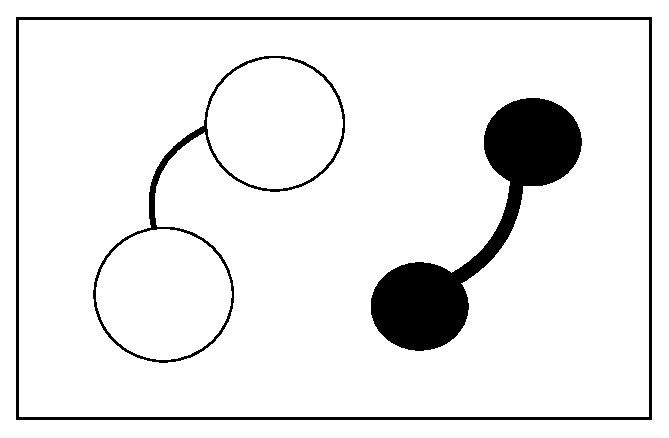
\includegraphics[width=0.25\textwidth]{figures/bivalent2}
%	\caption{Bivalent System.}
%\end{figure}
%Accordingly, given a structure of multivalent receptors, it sounds plausible to design fitting ligands, i.e. ligands of the same valency.  %multivalent
%\\

%bind to monovalent or multivalent receptors?
Especially the bivalent or polyvalent case often is observed in nature. \marginpar{?}
These systems are of significant interest for pharmaceutical and technical applications. If the ligands are linked to each other in an appropriate way to match the preorganized receptor molecules and, thus, are also presented multivalently, then extremely high binding affinities are often observed, which is conjectured to originate by the rebinding effect. %be caused
\begin{figure}[!ht]
	\centering
	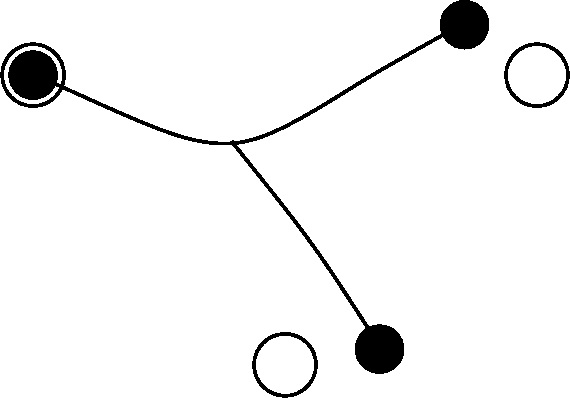
\includegraphics[width=0.25\textwidth]{figures/trivalent_binding.jpg}
	\caption{Trivalent System.}
	\label{fig:trivalent}
\end{figure}
%For the monovalent case, the mathematical modeling of its kinetics is well understood. monovalent = reversible? or why not of interest??? -> trivial min. reb. eff
This is clarified in figure \ref{fig:trivalent}, representing a trivalent system. If one of the connected ligands dissociated from its receptor, after being in the completely bound state (triple bound), then the probability of the ligand to be still close to its receptor and to rebind, is high.
We can imagine that this rebinding effect is even higher than it would have been the case in a monovalent system, since the ligand is kept at its place by its two connected ligands.
%after that the trivalent ligand was completely bound to the trivalent receptor, 

The strength of this ``adherence'' depends also from the flexibility of the linker. They can be either rigid/stiff or more flexible. A rigid linker holds the connected ligand more strongly at its place than a flexible linker. This relation is shown by Weber et al\cite{weber2012}. 
\\

The mathematical modelling of a monovalent system is well understood. Furthermore, if defined on the two macro states ``unbound'' and ``bound'', the computation of the minimal rebinding effect in such a system yields only the trivial solution, by theorem \ref{thm:reversible_trivial}.

Hence, as the the easiest multivalent case, we consider a \textbf{bivalent} process.
Such a system can be described by three macro states: ``unbound'', ``singly bound'' and ``doubly bound'', depicted in figure \ref{fig:bivalent_states}. %modelled. shown/depicted
\begin{figure}[h] %[!ht]
	\centering
	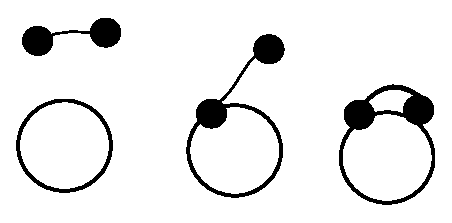
\includegraphics[width=0.4\textwidth]{figures/bivalent_states}
	\caption{Possible macro states of a bivalent system.}
	\label{fig:bivalent_states}
\end{figure}
This model can be represented by the reversible reactions
\begin{equation}
\begin{aligned}
\label{eq:reactions}
\mathrm{LL} + \mathrm{RR} & \rightleftharpoons \mathrm{L(LR)R}, \\
\mathrm{L(LR)R} & \rightleftharpoons \mathrm{(LRLR)}, \\
\mathrm{LL} + \mathrm{RR} & \rightleftharpoons \mathrm{(LRLR)},
\end{aligned}
\end{equation}
resulting in a transition rate matrix
\begin{equation*}
Q_c = 
\begin{pmatrix}
	-(k_{01} + k_{02})[RR]	& k_{01}[RR] 		 & k_{02}[RR]  \\
	k_{10}      			& -(k_{10} + k_{12}) & 	k_{12}	\\
	k_{20}					&	k_{21}			 & -(k_{20} + k_{21})
\end{pmatrix},
\end{equation*}
depending on the concentrations of the bivalent receptor molecules $[RR]$.
This matrix is constructed in the same fashion as explained in section \ref{sec:rebinding} for the monovalent case and as well describes changes of concentrations by the ordinary differential equation
\begin{equation*}
\dot{x}^T = x^T Q_c.
\end{equation*}
By this equation, changes of concentrations $x^T = ([LL], [L(LR)R], [(LRLR)])$ in this system can be observed/described.
\\

We can either measure or determine some plausible/feasible association/dissociation constants.
Remark: the last reaction equation in \eqref{eq:reactions} should have \textbf{very} small association and dissociation constants, since transitions from the unbound state directly to the bound state or vice versa are not realistic; if they happen then extremely rarely. However, we don't set them $0$, in order to avoid a sparse transition rate matrix $Q_c$.
%since we don't want to have a sparse transition rate matrix. %in order to get plausible/feasible results

\subsubsection*{Rebinding Effect}

We are in the situation that we are given a process which can be \textbf{interpreted} as a projection, while we do \textbf{not} know the original process and therefore cannot compute the actual rebinding effect.
However, we assume that by the unknown projection, there is some rebinding effect included in $Q_c$.
Assuming that it is clustered in terms of overlapping membership functions $\chi = XA$, we again solve optimization problem \eqref{eq:optimization} to derive the minimal rebinding effect as an estimation. \marginpar{Schur}
%In order to estimate it, we come back to compute the minimal rebinding effect.
\\

Need: eigenvectors/Schur vectors of $Q_c$ in order to compute the minimal rebinding effect included in this system.
It does not play a role if the original system was reversible or non-reversible, since we use Schur vectors to solve this problem.
\\

When is $Q_c$ reversible or non-reversible?
\\

%deeper/better understand
%In order to understand such a system, 
We consider it at first as an artificial system, by inserting convenient association and dissociation constants in order to obtain general informations about bivalent systems. Afterwards we examine a real system.
\subsubsection*{Artificial Binding Process}

First try: choice as in Weber and Fackeldey\cite{weber2014}.
\begin{itemize}
	\item For the reaction ``unbound'' $\leftrightarrow$ ``singly bound'': very high association $k_{01}$, low dissociation $k_{10}$
	\item For the reaction ``singly bound'' $\leftrightarrow$ ``doubly bound'': high association $k_{12}$, very low dissociation $k_{21}$
	\item For the reaction ``unbound'' $\leftrightarrow$ ``doubly bound'': very low association $k_{02}$, very low dissociation $k_{20}$
\end{itemize}

These parameters describe a system with desirable properties, since we want to obtain a high occupation of the receptors. %want to obtain/reach/achieve a high occupation
%It is a system where 
Unbound ligands have a strong preference to the single bound state, while dissociations do not happen often.
From the singly bound state to the doubly bound state happens still quite often, while dissociating not.
Going directly from unbound to doubly bound and vice versa can almost be neglected.

\begin{figure}[!ht]
	\label{fig:concentration_rebinding}
	\centering
	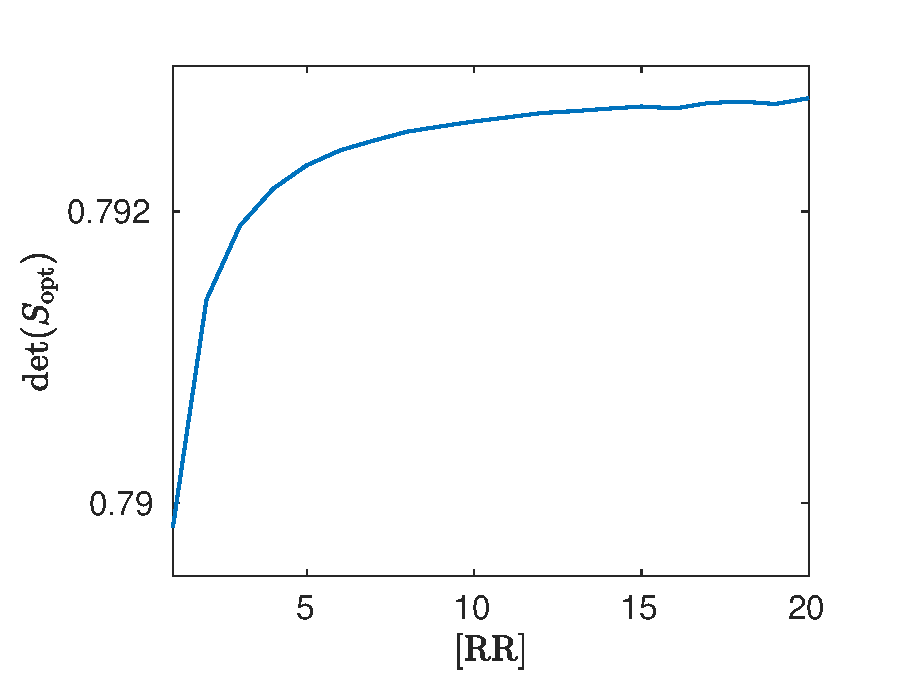
\includegraphics[width=0.55\textwidth]{figures/bivalent/concentration_rebinding}
	\caption{The minimal rebinding effect of $Q_c$ depending on the concentration $\mathrm{[RR]}$ of receptor molecules.}
\end{figure}

%Even though the difference of $\det(\Sopt)$ is not very large, we can clearly see a tendency of ..

In figure \ref{fig:concentration_rebinding}, we see that with increasing concentration of receptor molecules, the minimal rebinding effect decreases.
Even though the resulting difference of $\det(\Sopt)$ is not very large, this tendency is unambiguous. \marginpar{included in model?}
That makes sense: in a system with a large concentration of receptors, a ligand dissociating from a receptor is more likely to be already close to another receptor. If they bind, rebinding is prevented.
%Though have to keep in back-mind that the estimation can be rather good or rather bad..
\\

Even though this result qualitatively makes sense, it \textbf{should not}.
%The model consisting of the states ``unbound'', ``singly bound'' and ``doubly bound'' cannot distinguish if a dissociated ligand binds again
The model \eqref{eq:reactions} cannot distinguish if a dissociated ligand rebinds to its receptor or if it binds to a close receptor.
\\

Accordingly to Weber and Fackeldey\cite{weber2014}, this decreasing rebinding effect represented in figure \ref{fig:concentration_rebinding} can be explained by a decrease in the transition regions between the binding events caused by the increased receptor concentration.
\\

For \textbf{low} receptor concentrations the result is plausible; bindings shortly after a dissociation are likely to be a \textbf{rebinding}, since there are no other receptors nearby.
However, in realistic models the receptor concentration is higher.
\\

%Can binding events between different receptors be distinguished in the model \eqref{eq:reactions}?

%If not..
We need better models in order to correctly include rebinding effects. How?
%in order to correctly include rebinding effects in a model
\\

The presented model does not include enough informations/states to distinguish between a rebinding and a normal binding, since a dissociated ligand possesses no memory about the previous binding.
How could that be included?
Some approaches
\begin{itemize}
	\item considering larger systems, i.e. systems with more informations/ more states than just ``bound'', ``singly bound'', ``doubly bound'', making it possible to distinguish between rebinding and other bindings
	\item switching from the molecular kinetic to the molecular dynamic point of view: informations about the rebinding effect could be detected by simulations; i.e. generate a trajectory and analyze it for rebinding events \marginpar{Bettina Keller}
\end{itemize}
Finally one further outlook would be to compute the rebinding effect for time-dependent systems as well\cite{fackeldey2017}.
Consequent enhancement of PCCA+. Recently improved to non-reversible processes. New extension: including time-dependent systems by coherent sets (metastable sets with time) \cite{weber2017coherent}.

%\subsubsection*{Real existing binding process}
\subsubsection*{Real Binding Process}

Something with low receptor-concentrations.
\\

Picture

%%Remark: chemical processes are often \textbf{non-reversible}, see Fackeldey and Weber\cite{fackeldey2017}.
\newpage
  %\section{Transition Rate Matrix from Raman Data}

%The Rebinding Effect (=Recrossing Effect) occurs by the projection of a process onto a subspace. Thus, its consequences are not only visible in the particular example of a receptor-ligand system, but also in any other kind of processes. We present one example from the topic of Raman spectroscopy. It uses scattering methods (laser on molecule) in order to identify molecules and their chemical bonding.

We are given the transition matrix
\begin{equation*}
P_c = 
\begin{pmatrix}
8.0832573e-001 & 2.4773678e-001 & -5.6062515e-002 \\
2.9917361e-002 & 9.7916849e-001 & -9.0858553e-003 \\
1.8024711e-002 & -5.3149044e-003 & 9.8729019e-001
\end{pmatrix}.
\end{equation*}

Theoretically, the corresponding transition rate matrix $Q_c$ should be independent of time. But for our computations, it is impossible to make the time infinitesimal small. That's why we have to choose a certain (small) lag-time, on which the transition rate matrix will be defined.
For a lag-time $t = 0.05$(?), we compute $Q_c$ in order to solve the optimization problem \eqref{eq:optimization} for the rebinding effect.
  %\section{Transition Rate Matrix describing movement of electrons}
%\section{Movement of electrons}
%\section{Electron densities}
\section{Analysis of a Chemical Reaction}

Since each clustered matrix can be written as $S\inv T$, with the familiar meaning of $S$ as overlap matrix and $T$ as coupling matrix, we can deduce that \textbf{each} clustered system possesses some kind of (more or less) rebinding effect (not only restricted to receptor-ligand systems).
The meaning of this effect has to be interpreted for each system individually.
We present a different system (chemical/physical), describing the movement of electron densities of a given molecule.
\\

Formic acid is a molecule consisting of one carbon atom $C$, two oxygen atoms $O$ and two hydrogen atoms $H$.
In hydrocarbons and in the vapor phase, it consists of hydrogen-bonded dimers rather than individual molecules. \marginpar{ref}

In such a system, reactions between the individual molecules can be take place. An $H$ atom which is attached to an $O$ atom/nucleus moves to the $O$ atom of another molecule and vice versa.
These reactions are possible because of the (double) proton tunneling, see Schild\cite[Chapter 4]{schild2013}. \marginpar{ref} %caused/provoked
According to these reactions, changes in the electron density can be observed. %observed/computed
\\

Why is this electron density $\pi(t)$ time-dependent? \marginpar{pericyclic} \marginpar{metastable sets} \marginpar{coherent sets}

\begin{figure}[!ht]
	\centering
	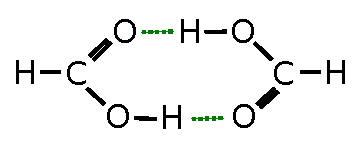
\includegraphics[width=0.4\textwidth]{figures/formic_acid_dimer.eps}
	\caption{Electron densities are measured in a system of formic acid dimers.}
	\label{fig:acid_dimer}
\end{figure}


%measured/computed(?)
Such a system can be described by a Markov chain, where the transition matrix $P$ consists of the (time-dependent) electron densities. %possible b/c electron densities sum up to 1???
Each of the different time-steps yields its own transition matrix. Then $P$ can be constructed of these matrices such that it is reversible.
 
 As $P$ is compound of several transition matrices, it possesses many dominant eigenvalues. However, for each of the individual transition matrices, $4$ metastable regions can be identified. 
%Electron densities of these reactions have been measured/computed(?) and can be described by a Markov chain
Clustering $P$ into $4$ metastable sets using PCCA+ yields the following transition rate matrix: %(though many large eigenvalues?)
%The following transition rate matrix has been obtained from a large reversible process by clustering with PCCA+:
%from experimental data by clustering with PCCA+:
\begin{equation*}
Q_c = 
\begin{pmatrix}
-2.0040  &  1.6859  &  0.1490  &  0.1690 \\
1.6192 &  -2.0010  &  0.1724  &  0.2095  \\
0.1451  &  0.1747 &  -1.9548  &  1.6350  \\
0.1632  &  0.2106  &  1.6217  & -1.9955
\end{pmatrix}.
\end{equation*}
Since it has been clustered with PCCA+, we assume that this system includes/contains \textbf{no} large rebinding effect (objective of PCCA+: make membership functions as crisp as possible).
Applying optimization problem $\eqref{eq:optimization}$ to this matrix, we find out that the minimal rebinding effect included in this system is given by
%\begin{equation*}
%	\det(\Sopt) = 0.9994,
%\end{equation*}
\begin{equation*}
\det(\Sopt) = 1,
\end{equation*}
and thus the optimal overlap matrix is the identity matrix.
\\

Unfortunately, this bound gives us no information about how much rebinding is obtained by the clustering.
This bound can be explained by the reversibility of the clustered system, $\Vert DQ_c - Q_c^T D \Vert_1 = 0$, and theorem \ref{thm:reversible_trivial}.
\\

However, from observing the given membership functions $\chi$ in figure \ref{fig:electron_membership}, we notice that they are not very crisp, but rather overlapping. %can already see
\begin{figure}[!ht]
	\centering
	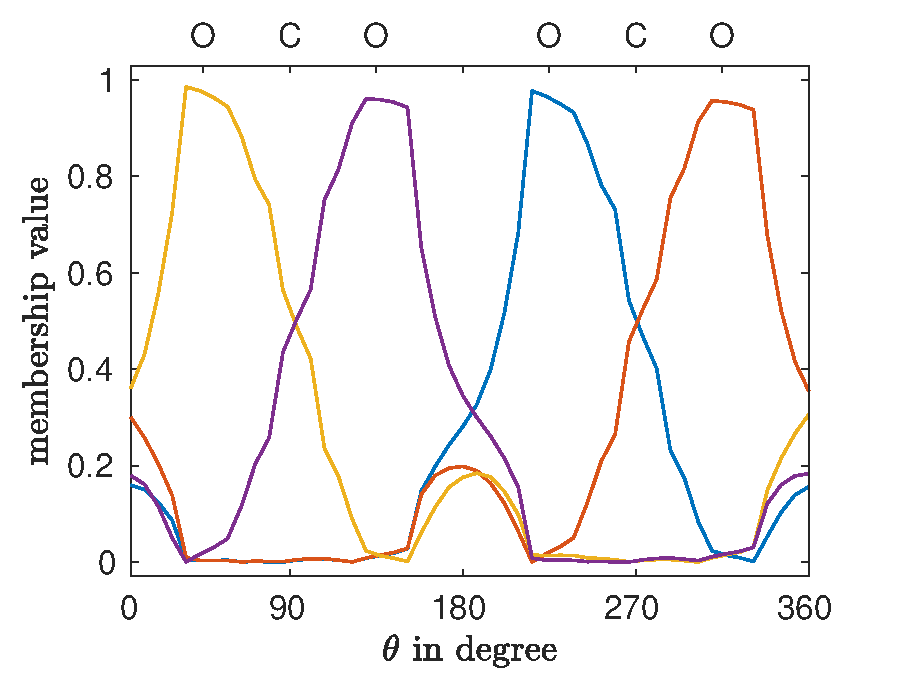
\includegraphics[width=0.6\textwidth]{figures/electrons/electrons_membership2.eps}
	\caption{Membership functions created by PCCA+}
	\label{fig:electron_membership}
\end{figure}

%However, since we are given the membership functions $\chi$ and the stationary distribution $\pi$ of the original process, 
Knowing the membership functions $\chi$ and the stationary distribution $\pi$ of the original process, we can compute the \textbf{real} rebinding effect by
\begin{equation*}
%S = D\inv \chi^T \diag(\pi, \dots, \pi_{500}) \chi.
\Sreal = D\inv \langle \chi, \chi \rangle_\pi
\end{equation*}
and thereby obtain
\begin{equation*}
\det(\Sreal) = 0.2925.
\end{equation*}

We have already seen before, that the minimal rebinding $\det(\Sopt)$ is not always a good estimation for the real rebinding and in particular is useless if the clustered process is reversible. %especially for systems close to reversible

However, it is astonishing that in this clustered system, there is actually so much real rebinding included. That was unexpected, since clustering with PCCA+ aims for rather crisp membership functions which would result in few rebinding.

Thus, even though the estimation $\det(\Sopt)$ was bad in that example, we can interpret the meaning of the actual rather high rebinding caused by the clustering.

%Ausblick: time-dependent clustering.. i.e. PCCA+ can yield different membership functions, making the Q_c more non-reverible sometimes and then implying a slightly better estimation for rebinding

%This example represents the existence of the rebinding effect in any kind of clustered processes.
%Originally, it was motivated by receptor-ligand systems, but is also occurs in other systems.
%Depending on the system the meaning of ``rebinding'' has to be interpreted corresponding to the context.
In that example, movements of electron densities around a given molecule have been considered.
%Thus, a strong overlap (=strong rebinding) can be explained by ...
The existence of the $4$ metastable conformations located around the $O$-molecules is plausible, since hydrogen is attracted to $O$.
However, these conformations are strongly overlapping. That can be explained by the rebinding effect. A hydrogen atom which is about to leave its $O$-atom and wandering to the next, possesses still a large probability to ``go back''/return to its original connected $O$.

%\begin{figure}[!ht]
%	\centering
	%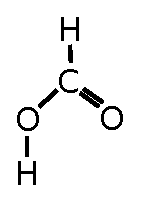
\includegraphics[width=0.1\textwidth]{figures/formic_acid.eps}
%	\includegraphics[width=0.6\textwidth]{figures/electrons/electrons_membership.eps}
%	\caption{Membership functions created by PCCA+}
%	\label{fig:electron_membership}
%\end{figure}

%electron density = describes trajectories of electrons (aufenthaltsdauer/ Zerfallsrate)


%This bound, being really high, gives us only few informations about the real rebinding effect; it could be either large or small.
%In this case, we didn't get much information from the optimization problem, even though the examined system is to a rather large extent non-reversible:
%\begin{equation*}
%	D Q_c = 
%	\begin{pmatrix}
%		-2.0249  &  1.6911  &  0.1547  &  0.1792 \\
%		1.6154 &  -1.9846  &  0.1743  &  0.1949  \\
%		0.1500  &  0.1769  & -1.9608  &  1.6339  \\
%		0.1725  &  0.1964  &  1.6225 &  -1.9915
%	\end{pmatrix}
%\end{equation*} vs
%\begin{equation*}
%	Q_c^T D = 
%	\begin{pmatrix}
%	  -0.0250  &  0.0209 &   0.0019 &   0.0022 \\
%	  -0.0316  &  0.0388 &  -0.0034 &  -0.0038 \\
%	  -0.0721  & -0.0850  &  0.9421 &  -0.7850 \\
%	  0.0841  &  0.0958  &  0.7912  & -0.9711
%	\end{pmatrix}
%\end{equation*}
%and the resulting deviation %\marginpar{which norm?}
%\begin{equation*}
%\Vert DQ - Q_c^T D \Vert_1 = 1.7577.
%\end{equation*}
%In order to evaluate the quality of this bound, we compare it to the real rebinding effect $\det(S_{\textrm{real}})$ obtained by the membership functions which has been used to perform this clustering. Since the original process and the membership functions (by PCCA+) are known, it is possible to compute the real rebinding effect.
\newpage

%What is the meaning of this matrix and of the included rebinding effect?

\addchap{Conclusion and Outlook}
  
\subparagraph*{Summary}
We have seen how we can get from a continuous stochastic process to a finite process defined on its metastable sets.
%role/differences
The relevance of metastability and the differences between reversible and nonreversible processes have been highlighted, in order to solve an optimization problem for both kind of processes in a given molecular system.

The rebinding effect included in a receptor-ligand system stems from the projection onto a finite state space.
%importance/meaning/relevance
Its relevance is justified by its influence to the stability of this system. That means that a high rebinding effect increases the binding affinity of a process, which is relevant for applications like (computational) drug design where it is important to predict the exact binding affinity of ligands.

\subparagraph*{Role of overlap matrix}
We want to highlight the role of the matrix $S$, from theorem \ref{thm:galerkin}, which is used to measure the rebinding effect.
In chapter \ref{chap:markov}, it has been introduced mathematically as a part of the matrix representation of a clustered Markov process. It basically consists of the scalar products of the different membership functions representing the macro states. %statistical weights. representing/corresponding to
In chapter \ref{chap:meta}, we have seen its relation to the overlap of the membership functions, that is $S$ can be interpreted as an ``overlap matrix'', containing information about the degree of fuzzyness of the clustering.
In chapter \ref{chap:rebinding}, we stated a lower bound for the rebinding effect in terms of the matrix $S$.
We have seen that a high rebinding effect, and thus strongly overlapping membership functions (information encoded in $S$), result in a more stable system. Thus, $S$ influences the metastability of a given system.
\noindent\fbox{%
	\parbox{\textwidth}{%
		Rebinding Effect $\leftrightarrow$ Overlap of Membership Functions (=Degree of fuzzyness) $\leftrightarrow$ Stability of System $\leftrightarrow$ Degree of Nonreversibility?
	}%
}
%(=Degree of Fuzzyness)
%=higher binding affinity

\subparagraph*{Role of Nonreversibility}

%rebinding effect vanishes
In a reversible system, the minimal rebinding effect is always given by $\det(S_{\textrm{opt}}) = 1$, meaning that there is no rebinding. Such a clustering in metastable sets is hard and not fuzzy and therefore not recommended. As described in chapter \ref{chap:meta}, some overlap in the clustering is good.

In a nonreversible system however, the minimal rebinding effect is higher, meaning that the clustering includes some overlap.
The higher the nonreversibility of a system, the higher the minimal rebinding effect and thus, the higher the overlap of the membership functions.

%\subparagraph*{Role of Multivalence}  
  \newpage
  \chapter*{Outlook} %aktueller Stand der Forschung
%As the main topics of this thesis are current research topics, we give a short outlook of the current projects etc...

This thesis combines two research topics that are highly discussed recently.
%Firstly, the general field of molecular design with its particular applications like drug design and the rebinding effect...
The general field of molecular design, in particular applications in drug design like the rebinding effect, as well as the analysis of nonreversible processes are ongoing research topics with 


\subparagraph*{Molecular Design}

Recently: reduction of dimension using metastable decompositions (PCCA+) helped to perform simulations which would have been impossible on the larger (cont.) state space.

Outlook: But still it is only possible to simulate on ...timescales.. longer timescales like several seconds, like needed for protein folding etc, are still infeasible, but with increasing computing power of supercomputers become more and more realistic.

(Noe Weber..)

\subparagraph*{Rebinding Effect}

In order to design drug molecules, it is important to know the exact binding affinity of a given system (set of ligands). Therefore the knowledge of the occuring rebinding effect can help to improve this design process/..

\subparagraph*{Multivalence}

The kinetics and design of multivalent processes is a current research project of the ``Computational Molecular Design'' group at ZIB.

\subparagraph*{Nonreversible Processes}
%Schur Decomposition

The study of reversible processes is very advanced/well-established, based on eigendecomposition. %study/analysis. approach/idea
The idea to apply a Schur Decomposition instead has been proposed by Röblitz and further promoted by Weber. This generalized approach includes the special case of non-reversible processes and thus could become the generalized approach to analyze stochastic processes. %improved/enhanced/...

%Like it has been the case for reversible processes, the Schur decomposition approach could be stretched out to continuous processes, also including nonreversible transfer operators.

In general, the research of non-reversible processes is rather at the beginning. Using Schur Decomposition could yield many results for those processes.

Many processes occuring in real life are nonreversible (which ones?).

%As in real life, there are many nonreversible processes and, like in the example of the rebinding effect, which can only be reasonably bounded for nonreversible processes, the examination of such processes is crucial. The Schur Decomposition, as a generalization of the eigendecomposition, seems to be an appropriate approach to tackle this problem.
%Though it has to be developed more elaborated, like for continuous processes, as this topic has just begun to raise.
%It has been first proposed by Röblitz in her dissertation and been further advances by Weber (ZIB report).

\subparagraph*{Time-Dependent Processes: Coherent Sets}

\subparagraph*{``Rebinding Effect'' for other processes}
The Rebinding Effect, or Recrossing Effect, can occur if we project a process. Thus, rebinding or recrossing events can happen in all other kind of processes. What is the role of it for these processes? \marginpar{examples}
%in the way we presented in 1.3
For this reason, we brought up the topic of Raman spectroscopy.

%3 sehr aktuelle Themen in dieser Arbeit: Rebinding Effect, SchurDecompop of a process, Application: Raman Spectroscopy

\cleardoublepage

%\appendix
%	\chapter{Minimal Rebinding Effect for reversible and non-reversible Processes}
%	%\subsection{Minimal rebinding effect: Optimization problem in terms of eigenvectors (reversible)}

%\section{\fontsize{12}{15}\selectfont Introduction}
\subsection*{A.1. Optimization problem in terms of eigenvectors: reversible system}

\begin{figure}[h]
	%\label{fig:reb_example}
	\centering
	\subfigure[The minimal rebinding effect compared to the degree of non-reversibility of the clustered system $Q_c$.]{\includegraphics[width=0.46\textwidth]{figures/rebinding/200_random/reb_opt_nonrev_200_random.eps}}
	\subfigure[The minimal and the real rebinding effect compared to the degree of non-reversibility of the clustered system $Q_c$.]{\includegraphics[width=0.46\textwidth]{figures/rebinding/200_random/reb_nonrev_200_random.eps}}
	%, increasing the probability of a fast \textbf{rebinding}.
	\hspace{20pt}
	\subfigure[The minimal rebinding effect $\det(\Sopt)$ compared to the real rebinding effect $\det(\Sreal)$ included in $Q_c$.]{\includegraphics[width=0.46\textwidth]{figures/rebinding/200_random/reb_200_random.eps}}
	\caption{The system described by the transition matrix $P$ is clustered with $200$ randomly generated feasible transformation matrices $A$.} % in order to compare some important parameters
\end{figure}
\newpage

\subsection*{A.2. Optimization problem in terms of Schur vectors: reversible}
\begin{figure}[h]
%	\label{fig:reb_example_nonrev}
	\centering
	\subfigure[The minimal rebinding effect compared to the degree of non-reversibility of the clustered system $Q_c$.]{\includegraphics[width=0.46\textwidth]{figures/rebinding/200_random_schur/reb_opt_nonrev_200_random.eps}}
	\subfigure[The minimal and the real rebinding effect compared to the degree of non-reversibility of the clustered system $Q_c$.]{\includegraphics[width=0.46\textwidth]{figures/rebinding/200_random_schur/reb_nonrev_200_random.eps}}
	%, increasing the probability of a fast \textbf{rebinding}.
	\hspace{20pt}
	\subfigure[The minimal rebinding effect $\det(\Sopt)$ compared to the real rebinding effect $\det(\Sreal)$ included in $Q_c$.]{\includegraphics[width=0.46\textwidth]{figures/rebinding/200_random_schur/reb_200_random.eps}}
	\caption{The system described by the transition matrix $P$ is clustered with $200$ randomly generated feasible transformation matrices $A$ for the values $\epsilon = 0$, $\delta = 0$.} % in order to compare some important parameters
\end{figure}
\newpage

\subsection*{A.3. Optimization problem in terms of Schur vectors: non-reversible, real eigenvectors}
\begin{figure}[h]
	%	\label{fig:reb_example_nonrev}
	\centering
	\subfigure[The minimal rebinding effect compared to the degree of non-reversibility of the clustered system $Q_c$.]{\includegraphics[width=0.46\textwidth]{figures/rebinding/200_random_schur/epsilon0.004/reb_opt_nonrev_200_random.eps}}
	\subfigure[The minimal and the real rebinding effect compared to the degree of non-reversibility of the clustered system $Q_c$.]{\includegraphics[width=0.46\textwidth]{figures/rebinding/200_random_schur/epsilon0.004/reb_nonrev_200_random.eps}}
	%, increasing the probability of a fast \textbf{rebinding}.
	\hspace{20pt}
	\subfigure[The minimal rebinding effect $\det(\Sopt)$ compared to the real rebinding effect $\det(\Sreal)$ included in $Q_c$.]{\includegraphics[width=0.46\textwidth]{figures/rebinding/200_random_schur/epsilon0.004/reb_200_random.eps}}
	\caption{The system described by the transition matrix $P$ is clustered with $200$ randomly generated feasible transformation matrices $A$ for the values $\epsilon = 0.004$, $\delta = 0$.} % in order to compare some important parameters
\end{figure}
\newpage

%\subsection*{Minimal rebinding effect: Optimization problem in terms of Schur vectors (non-reversible, complex eigenvectors)}
%\begin{figure}[h]
	%	\label{fig:reb_example_nonrev}
%	\centering
%	\subfigure[The minimal rebinding effect compared to the degree of non-reversibility of the clustered system $Q_c$.]{\includegraphics[width=0.46\textwidth]{figures/rebinding/200_random_schur/gamma0.01/reb_opt_nonrev_200_random.eps}}
%	\subfigure[The minimal and the real rebinding effect compared to the degree of non-reversibility of the clustered system $Q_c$.]{\includegraphics[width=0.46\textwidth]{figures/rebinding/200_random_schur/gamma0.01/reb_nonrev_200_random.eps}}
	%, increasing the probability of a fast \textbf{rebinding}.
%	\hspace{20pt}
%	\subfigure[The minimal rebinding effect $\det(\Sopt)$ compared to the real rebinding effect $\det(\Sreal)$ included in $Q_c$.]{\includegraphics[width=0.46\textwidth]{figures/rebinding/200_random_schur/gamma0.01/reb_200_random.eps}}
%	\caption{The system described by the transition matrix $P$ is clustered with $200$ randomly generated feasible transformation matrices $A$ for the values $\epsilon = 0$, $\delta = 0.01$.} % in order to compare some important parameters
%\end{figure}
%\newpage

\subsection*{A.4. Optimization problem in terms of Schur vectors: non-reversible, non-diagonalizable}
\begin{figure}[h]
	%	\label{fig:reb_example_nonrev}
	\centering
	\subfigure[The minimal rebinding effect compared to the degree of non-reversibility of the clustered system $Q_c$.]{\includegraphics[width=0.46\textwidth]{figures/rebinding/200_random_schur/epsilon0.004delta0.01/reb_opt_nonrev_200_random.eps}}
	\subfigure[The minimal and the real rebinding effect compared to the degree of non-reversibility of the clustered system $Q_c$.]{\includegraphics[width=0.46\textwidth]{figures/rebinding/200_random_schur/epsilon0.004delta0.01/reb_nonrev_200_random.eps}}
	%, increasing the probability of a fast \textbf{rebinding}.
	\hspace{20pt}
	\subfigure[The minimal rebinding effect $\det(\Sopt)$ compared to the real rebinding effect $\det(\Sreal)$ included in $Q_c$.]{\includegraphics[width=0.46\textwidth]{figures/rebinding/200_random_schur/epsilon0.004delta0.01/reb_200_random.eps}}
	\caption{The system described by the transition matrix $P$ is clustered with $200$ randomly generated feasible transformation matrices $A$ for the values $\epsilon = 0.004$, $\delta = 0.01$.} % in order to compare some important parameters
\end{figure}
\newpage

\subsection*{A.5. Optimization problem in terms of Schur vectors: non-reversible, complex eigenvectors}
\begin{figure}[h]
	%	\label{fig:reb_example_nonrev}
	\centering
	\subfigure[The minimal rebinding effect compared to the degree of non-reversibility of the clustered system $Q_c$.]{\includegraphics[width=0.46\textwidth]{figures/rebinding/200_random_schur/epsilon0.002gamma0.01/reb_opt_nonrev_200_random.eps}}
	\subfigure[The minimal and the real rebinding effect compared to the degree of non-reversibility of the clustered system $Q_c$.]{\includegraphics[width=0.46\textwidth]{figures/rebinding/200_random_schur/epsilon0.002gamma0.01/reb_nonrev_200_random.eps}}
	%, increasing the probability of a fast \textbf{rebinding}.
	\hspace{20pt}
	\subfigure[The minimal rebinding effect $\det(\Sopt)$ compared to the real rebinding effect $\det(\Sreal)$ included in $Q_c$.]{\includegraphics[width=0.46\textwidth]{figures/rebinding/200_random_schur/epsilon0.002gamma0.01/reb_200_random.eps}}
	\caption{The system described by the transition matrix $P$ is clustered with $200$ randomly generated feasible transformation matrices $A$ for the values $\epsilon = 0.002$, $\gamma = 0.01$.} % in order to compare some important parameters
\end{figure}
	%%\subsection{Minimal rebinding effect: Optimization problem in terms of eigenvectors (reversible)}

%\section{\fontsize{12}{15}\selectfont Introduction}
\subsection*{A.1. Optimization problem in terms of eigenvectors: reversible system}

\begin{figure}[h]
	%\label{fig:reb_example}
	\centering
	\subfigure[The minimal rebinding effect compared to the degree of non-reversibility of the clustered system $Q_c$.]{\includegraphics[width=0.46\textwidth]{figures/rebinding/200_eigen_vs_schur/eigen1.eps}}
	\subfigure[The minimal and the real rebinding effect compared to the degree of non-reversibility of the clustered system $Q_c$.]{\includegraphics[width=0.46\textwidth]{figures/rebinding/200_eigen_vs_schur/eigen2.eps}}
	%, increasing the probability of a fast \textbf{rebinding}.
	\hspace{20pt}
	\subfigure[The minimal rebinding effect $\det(\Sopt)$ compared to the real rebinding effect $\det(\Sreal)$ included in $Q_c$.]{\includegraphics[width=0.46\textwidth]{figures/rebinding/200_eigen_vs_schur/eigen3.eps}}
	\caption{The system described by the transition matrix $P$ is clustered with $200$ randomly generated feasible transformation matrices $A$.} % in order to compare some important parameters
\end{figure}
\newpage

\subsection*{A.2. Optimization problem in terms of Schur vectors: reversible}
\begin{figure}[h]
%	\label{fig:reb_example_nonrev}
	\centering
	\subfigure[The minimal rebinding effect compared to the degree of non-reversibility of the clustered system $Q_c$.]{\includegraphics[width=0.46\textwidth]{figures/rebinding/200_eigen_vs_schur/schur_rev1.eps}}
	\subfigure[The minimal and the real rebinding effect compared to the degree of non-reversibility of the clustered system $Q_c$.]{\includegraphics[width=0.46\textwidth]{figures/rebinding/200_eigen_vs_schur/schur_rev2.eps}}
	%, increasing the probability of a fast \textbf{rebinding}.
	\hspace{20pt}
	\subfigure[The minimal rebinding effect $\det(\Sopt)$ compared to the real rebinding effect $\det(\Sreal)$ included in $Q_c$.]{\includegraphics[width=0.46\textwidth]{figures/rebinding/200_eigen_vs_schur/schur_rev3.eps}}
	\caption{The system described by the transition matrix $P$ is clustered with $200$ randomly generated feasible transformation matrices $A$ for the values $\epsilon = 0$, $\delta = 0$.} % in order to compare some important parameters
\end{figure}
\newpage

\subsection*{A.3. Optimization problem in terms of Schur vectors: non-reversible, real eigenvectors}
\begin{figure}[h]
	%	\label{fig:reb_example_nonrev}
	\centering
	\subfigure[The minimal rebinding effect compared to the degree of non-reversibility of the clustered system $Q_c$.]{\includegraphics[width=0.46\textwidth]{figures/rebinding/200_eigen_vs_schur/schur_eps1.eps}}
	\subfigure[The minimal and the real rebinding effect compared to the degree of non-reversibility of the clustered system $Q_c$.]{\includegraphics[width=0.46\textwidth]{figures/rebinding/200_eigen_vs_schur/schur_eps2.eps}}
	%, increasing the probability of a fast \textbf{rebinding}.
	\hspace{20pt}
	\subfigure[The minimal rebinding effect $\det(\Sopt)$ compared to the real rebinding effect $\det(\Sreal)$ included in $Q_c$.]{\includegraphics[width=0.46\textwidth]{figures/rebinding/200_eigen_vs_schur/schur_eps3.eps}}
	\caption{The system described by the transition matrix $P$ is clustered with $200$ randomly generated feasible transformation matrices $A$ for the values $\epsilon = 0.004$, $\delta = 0$.} % in order to compare some important parameters
\end{figure}
\newpage

%\subsection*{Minimal rebinding effect: Optimization problem in terms of Schur vectors (non-reversible, complex eigenvectors)}
%\begin{figure}[h]
	%	\label{fig:reb_example_nonrev}
%	\centering
%	\subfigure[The minimal rebinding effect compared to the degree of non-reversibility of the clustered system $Q_c$.]{\includegraphics[width=0.46\textwidth]{figures/rebinding/200_random_schur/gamma0.01/reb_opt_nonrev_200_random.eps}}
%	\subfigure[The minimal and the real rebinding effect compared to the degree of non-reversibility of the clustered system $Q_c$.]{\includegraphics[width=0.46\textwidth]{figures/rebinding/200_random_schur/gamma0.01/reb_nonrev_200_random.eps}}
	%, increasing the probability of a fast \textbf{rebinding}.
%	\hspace{20pt}
%	\subfigure[The minimal rebinding effect $\det(\Sopt)$ compared to the real rebinding effect $\det(\Sreal)$ included in $Q_c$.]{\includegraphics[width=0.46\textwidth]{figures/rebinding/200_random_schur/gamma0.01/reb_200_random.eps}}
%	\caption{The system described by the transition matrix $P$ is clustered with $200$ randomly generated feasible transformation matrices $A$ for the values $\epsilon = 0$, $\delta = 0.01$.} % in order to compare some important parameters
%\end{figure}
%\newpage

\subsection*{A.4. Optimization problem in terms of Schur vectors: non-reversible, non-diagonalizable}
\begin{figure}[h]
	%	\label{fig:reb_example_nonrev}
	\centering
	\subfigure[The minimal rebinding effect compared to the degree of non-reversibility of the clustered system $Q_c$.]{\includegraphics[width=0.46\textwidth]{figures/rebinding/200_eigen_vs_schur/schur_del1.eps}}
	\subfigure[The minimal and the real rebinding effect compared to the degree of non-reversibility of the clustered system $Q_c$.]{\includegraphics[width=0.46\textwidth]{figures/rebinding/200_eigen_vs_schur/schur_del2.eps}}
	%, increasing the probability of a fast \textbf{rebinding}.
	\hspace{20pt}
	\subfigure[The minimal rebinding effect $\det(\Sopt)$ compared to the real rebinding effect $\det(\Sreal)$ included in $Q_c$.]{\includegraphics[width=0.46\textwidth]{figures/rebinding/200_eigen_vs_schur/schur_del3.eps}}
	\caption{The system described by the transition matrix $P$ is clustered with $200$ randomly generated feasible transformation matrices $A$ for the values $\epsilon = 0.004$, $\delta = 0.01$.} % in order to compare some important parameters
\end{figure}
%\newpage

%\subsection*{A.5. Optimization problem in terms of Schur vectors: non-reversible, complex eigenvectors}
%\begin{figure}[h]
	%	\label{fig:reb_example_nonrev}
%	\centering
%	\subfigure[The minimal rebinding effect compared to the degree of non-reversibility of the clustered system %$Q_c$.]{\includegraphics[width=0.46\textwidth]{figures/rebinding/200_random_schur/epsilon0.002gamma0.01/reb_opt_nonrev_200_random.eps}}
%	\subfigure[The minimal and the real rebinding effect compared to the degree of non-reversibility of the clustered system $Q_c$.]{\includegraphics[width=0.46\textwidth]{figures/rebinding/200_random_schur/epsilon0.002gamma0.01/reb_nonrev_200_random.eps}}
	%, increasing the probability of a fast \textbf{rebinding}.
%	\hspace{20pt}
%	\subfigure[The minimal rebinding effect $\det(\Sopt)$ compared to the real rebinding effect $\det(\Sreal)$ included in $Q_c$.]{\includegraphics[width=0.46\textwidth]{figures/rebinding/200_random_schur/epsilon0.002gamma0.01/reb_200_random.eps}}
%	\caption{The system described by the transition matrix $P$ is clustered with $200$ randomly generated feasible transformation matrices $A$ for the values $\epsilon = 0.002$, $\gamma = 0.01$.} % in order to compare some important parameters
%\end{figure}


\cleardoublepage
\newpage
\pagenumbering{roman}
\setcounter{page}{5}
%\input{./parts/eidesstattliche_erklaerung}
%\newpage
%\bibliographystyle{abbrv}
%\bibliographystyle{abbrvnat}
%\bibliographystyle{acm}
\bibliographystyle{siamplain}
\addcontentsline{toc}{chapter}{Bibliography}
\bibliography{bib/main.bib}
%\addcontentsline{totoc}{chapter}{Bibliography}

% \newpage
% \chapter{Source Code}
%  \input{./parts/source_code}

 \clearpage
 \section*{Selbstständigkeitserklärung}

Hiermit bestätige ich, dass ich die vorliegende Arbeit selbstständig verfasst habe und keine anderen als die angegebenen Quellen und Hilfsmittel benutzt habe. Die Arbeit wurde bisher in gleicher oder ähnlicher Form keiner anderen Prüfungskommission vorgelegt und auch nicht veröffentlicht.
\\[5ex]
Berlin, den 4. September 2017 %\\[6ex]
%\begin{tabular}{@{}l@{}}\hline
%	Susanne R\"ohl
%\end{tabular}

 \renewcommand{\arraystretch}{1.5}

\hspace*{\fill}\begin{tabular}{@{}l@{}}\hline
	\makebox[5cm]{Susanne R\"ohl}
\end{tabular}

%\begin{tabular}{lp{2em}l} 
%	\hspace{5cm}   && \hspace{4cm} \\\cline{1-1}\cline{3-3} 
%	Ort, Datum     && Unterschrift 
%\end{tabular}


%  \vspace{5\baselineskip} 
%  \noindent 
%  \rule[0.5ex]{25em}{0.5pt}\\ 
%  Ort, Datum\qquad\qquad Unterschrift 


\end{document}


